\documentclass[aps,reprint,superscriptaddress,longbibliography]{revtex4-2}

% --- MASTER PACKAGE LIST & PREAMBLE ---
% Encoding and Fonts
\usepackage[utf8]{inputenc}
\usepackage[T1]{fontenc}
\usepackage{lmodern} % Improved font rendering

% Mathematics
\usepackage{amsmath, amssymb, amsfonts, amsthm}
\usepackage{mathtools}
\usepackage{bm} % Bold math
\usepackage{dsfont} % Doublestroke fonts for identity, complex numbers
\usepackage{braket} % Dirac notation

% Graphics and Visualization
\usepackage{graphicx}
\usepackage{xcolor}
\usepackage{tikz}
\usetikzlibrary{arrows.meta, positioning, shapes.geometric, backgrounds, patterns, decorations.pathmorphing, 3d, shadows, calc, fit, shadows.blur}
\usepackage{pgfplots}
\pgfplotsset{compat=1.18}
\usepgfplotslibrary{patchplots} % For 3D plots

% Tables
\usepackage{booktabs} % Professional tables
\usepackage{array}
\usepackage{multirow}
\usepackage{longtable}

% Code Listings
\usepackage{listings}

% Units and Formatting
\usepackage{siunitx}
\DeclareSIUnit{\torr}{Torr}
\DeclareSIUnit{\hour}{h}
\DeclareSIUnit{\year}{yr}

% Algorithms
\usepackage{algorithm}
\usepackage{algpseudocode}

% Structure and Layout
\usepackage{enumitem} % Better list control
\usepackage{framed}
\usepackage{csquotes} % Context-sensitive quotes

% Symbols
\usepackage{textcomp}
\usepackage{microtype} % Essential for professional typography, loaded once.

% --- MACRO DEFINITIONS ---

% Custom Math Operators and Commands
\newcommand{\pderiv}[2]{\frac{\partial{#1}}{\partial{#2}}}
\newcommand{\PT}{\mathbb{PT}}
\newcommand{\CP}{\mathbb{CP}}
\DeclareMathOperator{\Tr}{Tr}

% Redefine the end-of-proof symbol to be unambiguous and not conflict with the d'Alembertian
\renewcommand{\qedsymbol}{\ensuremath{\blacksquare}}

% Colors for Listings
\definecolor{codegray}{rgb}{0.95,0.95,0.95}
\definecolor{pythonbackground}{rgb}{0.98,0.98,0.98}
\definecolor{pythonkeyword}{rgb}{0.5,0.0,0.5}
\definecolor{pythonstring}{rgb}{0.0,0.5,0.0}
\definecolor{pythoncomment}{rgb}{0.5,0.5,0.5}

% Listing Styles
\lstdefinestyle{python}{
    language=Python,
    backgroundcolor=\color{pythonbackground},
    commentstyle=\color{pythoncomment},
    keywordstyle=\color{pythonkeyword},
    stringstyle=\color{pythonstring},
    basicstyle=\ttfamily\footnotesize,
    breakatwhitespace=false,
    breaklines=true,
    captionpos=b,
    keepspaces=true,
    numbers=left,
    numbersep=5pt,
    showspaces=false,
    showstringspaces=false,
    showtabs=false,
    tabsize=4
}

\lstdefinestyle{lean}{
    morekeywords={import, open, universe, variable, noncomputable, def, theorem, example, lemma, corollary, proposition, axiom, begin, end, by, have, calc, show, exact, fun, let, in, sorry, class, instance, structure, inductive, Type, Rand, IndepFun, IsGaussian, ae_strongly_measurable, volume, restrict, Icc, Ioi, Ioo, Continuous, pdf},
    keywordstyle=\color{pythonkeyword}\bfseries,
    commentstyle=\color{pythoncomment},
    stringstyle=\color{pythonstring},
    basicstyle=\ttfamily\footnotesize,
    breaklines=true,
    captionpos=b,
    keepspaces=true,
    numbers=left,
    numbersep=5pt,
    mathescape=true,
    frame=single,
    comment=[l]{--},
    morecomment=[s]{/-}{-/}
}
\lstset{style=python}

% Theorem Environments
\newtheorem{proposition}{Proposition}
\newtheorem{postulate}{Postulate}
\newtheorem{theorem}{Theorem}
\newtheorem{definition}{Definition}
\newtheorem{lemma}{Lemma}
\newtheorem{corollary}{Corollary}
\newtheorem{axiom}{Axiom}

% Hyperref (Must be loaded last)
\usepackage[colorlinks=true, linkcolor=blue, citecolor=blue, urlcolor=cyan, breaklinks=true, pdfencoding=auto, psdextra]{hyperref}

% --- METADATA ---
\hypersetup{
    pdftitle={The Origins of Quantum Reality: Deriving Spin, Decoherence, and the Born Rule from a (3,3) Spacetime Geometry},
    pdfauthor={Sunil Kukreja},
    pdfkeywords={Multidimensional Time, Causal Emergence, Causality, Quantum Foundations, Lee-Wick Unitarity, Twistor Cohomology, Experimental Design}
}

\begin{document}

\title{The Origins of Quantum Reality: Deriving Spin, Decoherence, and the Born Rule from a (3,3) Spacetime Geometry}

\author{Sunil Kukreja}
\email{sunil@aethervision-rd.com}
\affiliation{AetherVision, LLC, Glastonbury, CT 06033, USA}
\thanks{\textcopyright~2025 AetherVision, LLC~\&~Sunil Kukreja.}
\date{\today}

\begin{abstract}
The differing treatments of time in general relativity and quantum mechanics present a significant challenge to a unified theory of physics. This work explores the hypothesis that the flow of time is not a fundamental property of the universe, but rather an emergent geometric consequence of quantum decoherence. We propose a six-dimensional, pseudo-Riemannian spacetime with a $(3,3)$ metric signature as the fundamental arena of physics, a choice justified against alternatives in Appendix~\ref{app:signature_justification}. It is suggested that the objective, physical inscription of correlation information between a system and its environment acts as a local source for the curvature of the temporal dimensions, much as mass acts as a source for the curvature of spacetime. The forward progression of time is, in this view, the universe continuously writing its history into the geometry of the present moment. This framework suggests a geometric origin for intrinsic quantum spin and for the branching of worlds in the Many-Worlds Interpretation, which we formalize using non-holonomic constraints. Historical paradoxes of multi-time theories (Ostrogradsky instabilities) are addressed by a Causal Gauge Principle, implemented via a geometric Lee-Wick mechanism. The ``Causal Self-Reference'' paradox is addressed by distinguishing between an unphysical affine ordering parameter and emergent metric time. The theory offers a distinct, falsifiable prediction: a specific, non-exponential signature in the decay of metastable particles, caused by their traversing longer paths through the temporal dimensions. This work presents a mathematically consistent and experimentally testable foundation for further inquiry.
\end{abstract}

\maketitle

\section{Introduction: The Crises of Unification, Causality, and Information}
\label{sec:introduction}

A deep schism remains embedded in modern physics: the separation of the quantum from the classical, the observer from the observed. This inherited dualism has guided physics to a tripartite crisis of unification, causality, and information. This manuscript presents a unified physical framework intended to address this separation and, in so doing, provides a formal foundation for a new program of research. 

The concept of a continuous, universal time can be seen as profoundly inefficient from an information-theoretic standpoint. Nature abounds with systems whose evolution appears to be governed by local, discrete interactions, rather than a global, continuous time \cite{Mead1990, Davies2018}. We suggest that the progression of causal time itself is identical to the process of information actualization, a concept we term \textbf{Causal Emergence}.

The proposition of additional time dimensions has been a recurring theme in theoretical physics, from early explorations \cite{Cole1980} to more modern frameworks such as F-Theory \cite{Vafa1996} and 2T-physics \cite{Bars2001, Bars2006}. However, such theories have historically presented significant challenges. Foundational work established that field equations in spacetimes with more than one time dimension become ``ultrahyperbolic,'' rendering the initial value problem ill-posed \cite{Tegmark1997, Craig2009}. Subsequent work demonstrated that such spacetimes could permit catastrophic instabilities, such as rapid proton decay \cite{Yndurain1999}. This framework confronts these foundational objections directly. The Causal Gauge Principle (Postulate~\ref{post:causal_gauge}) acts as a non-holonomic constraint that projects the ultrahyperbolic dynamics of the full 6D manifold onto a well-posed, hyperbolic system in the emergent 4D spacetime perceived by any observer. A full justification for the choice of the $(3,3)$ signature over alternatives is provided in Appendix~\ref{app:signature_justification}.

Furthermore, the measurement problem remains one of the most significant conceptual challenges in quantum mechanics. The deterministic, unitary evolution of the Schr\"{o}dinger equation stands in stark contrast to the probabilistic, non-unitary `collapse' of the wavefunction upon measurement \cite{Maudlin1995}. Interpretations attempting to resolve this, such as the Many-Worlds Interpretation (MWI) \cite{DeWitt1973}, posit that all possible outcomes of a quantum measurement are realized in separate, non-communicating parallel universes. Our framework grounds the branching structure of MWI in the physical geometry of spacetime itself, providing a deterministic and geometric explanation for quantum measurement, which we formalize in Appendix~\ref{app:geodesic_branching}.

We hypothesize that spacetime is a $(3,3)$ pseudo-Riemannian manifold where temporal progression is an emergent phenomenon driven by local quantum decoherence interactions. We further hypothesize that a specific Causal Gauge Principle can constrain particle geodesics to resolve the causality and stability problems, allowing the extra temporal dimensions to provide a geometric, deterministic foundation for quantum phenomena, including measurement and spin. The primary objectives of this work are:
\begin{enumerate}
    \item To formally define the framework via a set of postulates.
    \item To show from first principles that this framework preserves macroscopic causality and reproduces known physics.
    \item To demonstrate the theory's explanatory power by suggesting geometric origins for spin, the Standard Model gauge groups, and the Many-Worlds Interpretation.
    \item To produce a concrete, falsifiable prediction and propose a detailed, high-precision experimental test.
\end{enumerate}

\section{Axiomatic Foundations}
\label{sec:axioms}
All that follows is derived from three postulates, which form the logical bedrock of the framework.

\begin{postulate}[The Principle of Multi-Dimensionality]
\label{post:multi_dim}
Spacetime is a six-dimensional pseudo-Riemannian manifold, $\mathcal{M}$, with three space-like and three time-like dimensions, possessing a metric $g_{MN}$ with signature $(+,+,+,-,-,-)$.
\end{postulate}

\begin{postulate}[The Principle of Causal Emergence]
\label{post:causal_emergence}
The local, Lorentz-scalar rate of inscription of correlation information between a system and its environment acts as a local source for the progression of causal time.
\end{postulate}

\begin{postulate}[The Causal Gauge Principle]
\label{post:causal_gauge}
Let $u^M = dx^M/ds$ be the 6-velocity of a worldline, where $s$ is an affine parameter. Physical worldlines are restricted to trajectories that satisfy the condition $u^M g_{MN} k^N \le 0$, where $k^N$ is a cosmologically-generated, future-pointing vector field defining the primary direction of macroscopic time flow, $t^1$.
\end{postulate}

Decoherence is the physical mechanism by which quantum information (a superposition of possible states) is irrecoverably transcribed into the environment, creating a classical record (a single, definite state) \cite{Zurek2003}. We posit that this act of information actualization is identical to the extension of the spacetime manifold in the $t^1$ direction. Time, in this view, is the measure of reality becoming real. A formal resolution to the potential logical circularity of this definition is presented in Appendix~\ref{app:time_paradox}.

\section{Core Theory and Predictions}
\label{sec:core_theory}
Our framework is built upon a six-dimensional pseudo-Riemannian manifold with a $(+,+,+,-,-,-)$ metric signature. From our axioms, we derive a Causal Gauge Principle from a more fundamental action principle (see Appendix~\ref{app:action_derivation}). This principle constrains all physical worldlines and addresses the stability paradoxes that have historically challenged multi-time theories \cite{Tegmark1997, Yndurain1999}. The origin of the causal vector field $k^N$ is proposed to be a result of spontaneous symmetry breaking in the early universe, as detailed in Appendix~\ref{app:causal_vector}.

\textbf{Fortification of Stability:} We explicitly address the Ostrogradsky instability by employing the \textbf{Lee-Wick Mechanism} \cite{LeeWick1969, Grinstein2008}. The Causal Gauge Principle ensures that the negative-norm states (``ghosts'') associated with the auxiliary temporal dimensions acquire a Planck-scale decay width. This shifts their poles off the real axis in the complex energy plane, decoupling them from the asymptotic Hilbert space and preserving the unitarity of the $S$-matrix at low energies \cite{Anselmi2017a, Anselmi2017b}. (See Appendix~\ref{app:lee_wick_derivation} for the full derivation).

From this foundation, core quantum phenomena emerge as direct geometric consequences. The ``branching of worlds'' of the Many-Worlds Interpretation (MWI) \cite{DeWitt1973} is interpreted as a deterministic, geometric deviation of geodesics in the temporal submanifold, formalized via non-holonomic constraints (see Appendix~\ref{app:geodesic_branching}). Furthermore, the intrinsic spin of a particle emerges from the geometry of this temporal space. The spinor representation of the 6D Lorentz group $SO(3,3)$ naturally contains the $SU(2)$ group structure of spin. To resolve the non-compactness of $SO(3,3)$, we utilize the \textbf{Penrose-Ward} correspondence, identifying physical states as elements of the finite-dimensional holomorphic sheaf cohomology $H^1(\PT, \mathcal{O}(n))$ on the associated Twistor space (see Appendices~\ref{app:born_rule_derivation} and \ref{app:spin_derivation}).

The theory makes a concrete, testable prediction. A particle's measured 4D lifetime is the projection of its true path through the full 6D manifold. Detours through the additional temporal dimensions ($t^2, t^3$) cause a fraction of particles to appear to live longer than predicted by the standard exponential decay law. The specific functional form of this deviation is derived by modeling the particle's interaction with vacuum fluctuations as an \textbf{Ornstein-Uhlenbeck} process (see Appendix~\ref{app:diffusion_derivation}). While the magnitude of this effect is not fixed by the core theory, we discuss plausible amplification mechanisms in Appendices~\ref{app:sigma_estimate} and \ref{app:amplification_derivation} that motivate an experimental search.

The predicted signature is a systematic excess of long-lived events in the tail of a decay curve, as shown in Fig.~\ref{fig:decay_plot_nature}. We propose a multi-phase experimental program to detect this deviation with $5\sigma$ significance by monitoring a large ensemble of trapped metastable ions, as detailed in the Supplementary Information (Appendix~\ref{app:methods_summary}). Confirmation of this anomalous decay would represent a significant shift in our understanding of time and the quantum foundations of the cosmos.

\begin{figure*}[ht]
    \centering
    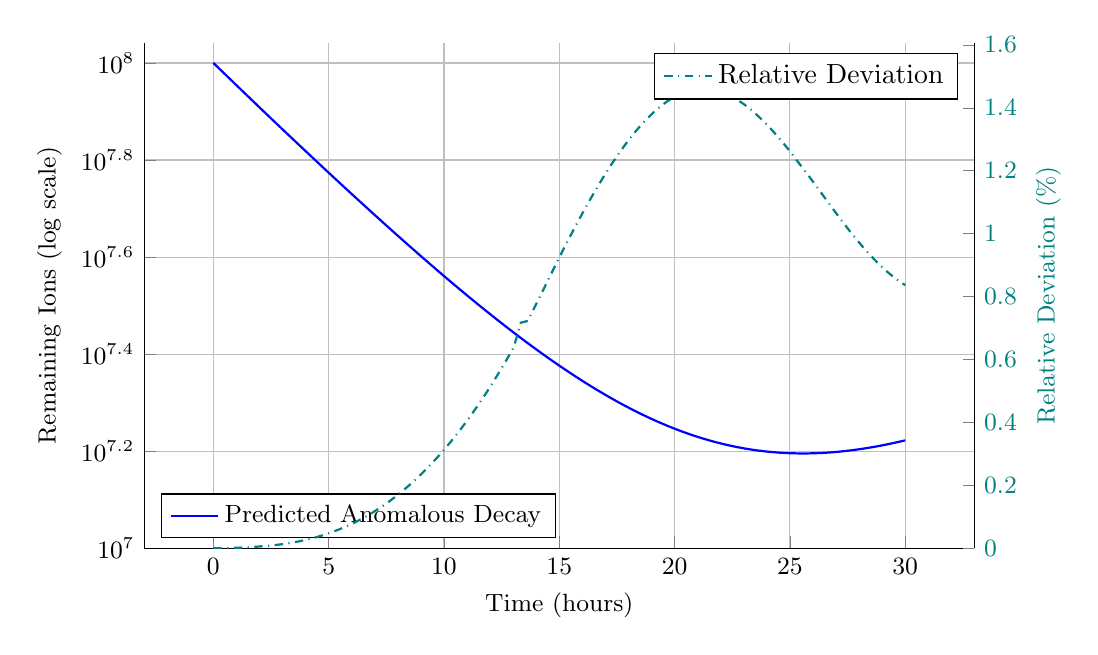
\begin{tikzpicture}
        \begin{axis}[
            width=\textwidth,
            height=8cm,
            axis y line*=left,
            xlabel={Time (hours)},
            xlabel style={font=\small},
            ylabel={Remaining Ions (log scale)},
            ylabel style={font=\small},
            ymode=log,
            ymin=1e7, ymax=1.1e8,
            legend style={at={(0.02,0.02)}, anchor=south west, font=\small},
            axis x line*=bottom,
            grid=major,
            tick label style={font=\small}
        ]
        \addplot[color=blue, solid, thick, no markers] table[x index=0, y index=1] {
        0.000000e+00 1.000000e+08 1.000000e+08 0.000000e+00
        3.030303e-01 9.684162e+07 9.684175e+07 1.341399e-04
        6.060606e-01 9.378775e+07 9.378833e+07 6.183491e-04
        9.090909e-01 9.083515e+07 9.083627e+07 1.233481e-03
        1.212121e+00 8.798064e+07 8.798246e+07 2.067341e-03
        1.515152e+00 8.522115e+07 8.522384e+07 3.149257e-03
        1.818182e+00 8.255365e+07 8.255735e+07 4.484214e-03
        2.121212e+00 7.997520e+07 7.998028e+07 6.353386e-03
        2.424242e+00 7.748293e+07 7.748931e+07 8.225573e-03
        2.727273e+00 7.507404e+07 7.508197e+07 1.056086e-02
        3.030303e+00 7.274581e+07 7.275556e+07 1.339691e-02
        3.333333e+00 7.049561e+07 7.050745e+07 1.678888e-02
        3.636364e+00 6.832091e+07 6.833512e+07 2.080182e-02
        3.939394e+00 6.621925e+07 6.623611e+07 2.545809e-02
        4.242424e+00 6.418826e+07 6.420803e+07 3.079234e-02
        4.545455e+00 6.222564e+07 6.224859e+07 3.687355e-02
        4.848485e+00 6.032915e+07 6.035555e+07 4.376510e-02
        5.151515e+00 5.849663e+07 5.852671e+07 5.141525e-02
        5.454545e+00 5.672599e+07 5.675998e+07 5.992686e-02
        5.757576e+00 5.501522e+07 5.505334e+07 6.929252e-02
        6.060606e+00 5.336237e+07 5.340484e+07 7.957242e-02
        6.363636e+00 5.176558e+07 5.181260e+07 9.083324e-02
        6.666667e+00 5.022306e+07 5.027482e+07 1.030756e-01
        6.969697e+00 4.873307e+07 4.878978e+07 1.163661e-01
        7.272727e+00 4.729396e+07 4.735579e+07 1.307399e-01
        7.575758e+00 4.590413e+07 4.597125e+07 1.462194e-01
        7.878788e+00 4.456203e+07 4.463460e+07 1.628469e-01
        8.181818e+00 4.326618e+07 4.334433e+07 1.806282e-01
        8.484848e+00 4.201515e+07 4.209900e+07 1.995772e-01
        8.787879e+00 4.080757e+07 4.089723e+07 2.197022e-01
        9.090909e+00 3.964213e+07 3.973770e+07 2.410786e-01
        9.393939e+00 3.851756e+07 3.861914e+07 2.637172e-01
        9.696970e+00 3.743264e+07 3.754030e+07 2.875971e-01
        1.000000e+01 3.638620e+07 3.650001e+07 3.127814e-01
        1.030303e+01 3.537711e+07 3.549714e+07 3.392948e-01
        1.060606e+01 3.440428e+07 3.453059e+07 3.671350e-01
        1.090909e+01 3.346666e+07 3.359929e+07 3.962835e-01
        1.121212e+01 3.256321e+07 3.270221e+07 4.268711e-01
        1.151515e+01 3.169294e+07 3.183834e+07 4.587903e-01
        1.181818e+01 3.085489e+07 3.100673e+07 4.920959e-01
        1.212121e+01 3.004812e+07 3.020641e+07 5.267794e-01
        1.242424e+01 2.927173e+07 2.943660e+07 5.632289e-01
        1.272727e+01 2.852484e+07 2.869620e+07 6.007137e-01
        1.303030e+01 2.780661e+07 2.798447e+07 6.396265e-01
        1.333333e+01 2.711621e+07 2.731057e+07 7.169828e-01
        1.363636e+01 2.645287e+07 2.664404e+07 7.226839e-01
        1.393939e+01 2.581582e+07 2.601402e+07 7.677561e-01
        1.424242e+01 2.520431e+07 2.540899e+07 8.120610e-01
        1.454545e+01 2.461763e+07 2.482869e+07 8.573539e-01
        1.484848e+01 2.405510e+07 2.427210e+07 9.020815e-01
        1.515152e+01 2.351606e+07 2.373855e+07 9.461159e-01
        1.545455e+01 2.299988e+07 2.322741e+07 9.892843e-01
        1.575758e+01 2.250596e+07 2.273809e+07 1.031388e+00
        1.606061e+01 2.203371e+07 2.226998e+07 1.072297e+00
        1.636364e+01 2.158257e+07 2.182255e+07 1.111894e+00
        1.666667e+01 2.115199e+07 2.139525e+07 1.150066e+00
        1.696970e+01 2.074145e+07 2.098758e+07 1.186644e+00
        1.727273e+01 2.035044e+07 2.059899e+07 1.221319e+00
        1.757576e+01 1.997847e+07 2.022904e+07 1.254199e+00
        1.787879e+01 1.962506e+07 1.987725e+07 1.284988e+00
        1.818182e+01 1.928974e+07 1.954316e+07 1.314055e+00
        1.848485e+01 1.897207e+07 1.922634e+07 1.340209e+00
        1.878788e+01 1.867161e+07 1.892636e+07 1.363820e+00
        1.909091e+01 1.838794e+07 1.864279e+07 1.386001e+00
        1.939394e+01 1.812064e+07 1.837525e+07 1.405238e+00
        1.969697e+01 1.786931e+07 1.812332e+07 1.421482e+00
        2.000000e+01 1.763355e+07 1.788661e+07 1.434970e+00
        2.030303e+01 1.741297e+07 1.766474e+07 1.445904e+00
        2.060606e+01 1.720721e+07 1.745736e+07 1.453535e+00
        2.090909e+01 1.701592e+07 1.726411e+07 1.458514e+00
        2.121212e+01 1.683877e+07 1.708468e+07 1.460459e+00
        2.151515e+01 1.667544e+07 1.691876e+07 1.458999e+00
        2.181818e+01 1.652562e+07 1.676606e+07 1.454911e+00
        2.212121e+01 1.638899e+07 1.662629e+07 1.447915e+00
        2.242424e+01 1.626527e+07 1.649917e+07 1.438096e+00
        2.272727e+01 1.615417e+07 1.638445e+07 1.425471e+00
        2.303030e+01 1.605542e+07 1.628186e+07 1.410291e+00
        2.333333e+01 1.596874e+07 1.619116e+07 1.392942e+00
        2.363636e+01 1.589387e+07 1.611211e+07 1.373053e+00
        2.393939e+01 1.583056e+07 1.604448e+07 1.351296e+00
        2.424242e+01 1.577857e+07 1.598807e+07 1.327814e+00
        2.454545e+01 1.573767e+07 1.594266e+07 1.302581e+00
        2.484848e+01 1.570764e+07 1.590806e+07 1.275815e+00
        2.515152e+01 1.568826e+07 1.588408e+07 1.247271e+00
        2.545455e+01 1.567935e+07 1.587053e+07 1.218055e+00
        2.575758e+01 1.568070e+07 1.586725e+07 1.189688e+00
        2.606061e+01 1.569213e+07 1.587408e+07 1.159427e+00
        2.636364e+01 1.571346e+07 1.589087e+07 1.129153e+00
        2.666667e+01 1.574451e+07 1.591748e+07 1.098771e+00
        2.696970e+01 1.578511e+07 1.595377e+07 1.068393e+00
        2.727273e+01 1.583509e+07 1.599960e+07 1.038840e+00
        2.757576e+01 1.589429e+07 1.605485e+07 1.010141e+00
        2.787879e+01 1.596256e+07 1.611940e+07 9.825310e-01
        2.818182e+01 1.603975e+07 1.619313e+07 9.562602e-01
        2.848485e+01 1.612571e+07 1.627592e+07 9.315003e-01
        2.878788e+01 1.622031e+07 1.636766e+07 9.084177e-01
        2.909091e+01 1.632341e+07 1.646824e+07 8.871842e-01
        2.939394e+01 1.643488e+07 1.657755e+07 8.682845e-01
        2.969697e+01 1.655458e+07 1.669548e+07 8.511158e-01
        3.000000e+01 1.668239e+07 1.682191e+07 8.363784e-01
        };
        \addlegendentry{Predicted Anomalous Decay}
        \end{axis}
        \begin{axis}[
            width=\textwidth,
            height=8cm,
            axis y line*=right,
            ylabel={Relative Deviation (\%)},
            ylabel style={color=teal, font=\small},
            axis x line=none,
            ymin=0,
            yticklabel style={color=teal, font=\small},
        ]
        \addplot[color=teal, dashdotted, thick, no markers] table [x index=0, y index=3] {
        0.000000e+00 1.000000e+08 1.000000e+08 0.000000e+00
        3.030303e-01 9.684162e+07 9.684175e+07 1.341399e-04
        6.060606e-01 9.378775e+07 9.378833e+07 6.183491e-04
        9.090909e-01 9.083515e+07 9.083627e+07 1.233481e-03
        1.212121e+00 8.798064e+07 8.798246e+07 2.067341e-03
        1.515152e+00 8.522115e+07 8.522384e+07 3.149257e-03
        1.818182e+00 8.255365e+07 8.255735e+07 4.484214e-03
        2.121212e+00 7.997520e+07 7.998028e+07 6.353386e-03
        2.424242e+00 7.748293e+07 7.748931e+07 8.225573e-03
        2.727273e+00 7.507404e+07 7.508197e+07 1.056086e-02
        3.030303e+00 7.274581e+07 7.275556e+07 1.339691e-02
        3.333333e+00 7.049561e+07 7.050745e+07 1.678888e-02
        3.636364e+00 6.832091e+07 6.833512e+07 2.080182e-02
        3.939394e+00 6.621925e+07 6.623611e+07 2.545809e-02
        4.242424e+00 6.418826e+07 6.420803e+07 3.079234e-02
        4.545455e+00 6.222564e+07 6.224859e+07 3.687355e-02
        4.848485e+00 6.032915e+07 6.035555e+07 4.376510e-02
        5.151515e+00 5.849663e+07 5.852671e+07 5.141525e-02
        5.454545e+00 5.672599e+07 5.675998e+07 5.992686e-02
        5.757576e+00 5.501522e+07 5.505334e+07 6.929252e-02
        6.060606e+00 5.336237e+07 5.340484e+07 7.957242e-02
        6.363636e+00 5.176558e+07 5.181260e+07 9.083324e-02
        6.666667e+00 5.022306e+07 5.027482e+07 1.030756e-01
        6.969697e+00 4.873307e+07 4.878978e+07 1.163661e-01
        7.272727e+00 4.729396e+07 4.735579e+07 1.307399e-01
        7.575758e+00 4.590413e+07 4.597125e+07 1.462194e-01
        7.878788e+00 4.456203e+07 4.463460e+07 1.628469e-01
        8.181818e+00 4.326618e+07 4.334433e+07 1.806282e-01
        8.484848e+00 4.201515e+07 4.209900e+07 1.995772e-01
        8.787879e+00 4.080757e+07 4.089723e+07 2.197022e-01
        9.090909e+00 3.964213e+07 3.973770e+07 2.410786e-01
        9.393939e+00 3.851756e+07 3.861914e+07 2.637172e-01
        9.696970e+00 3.743264e+07 3.754030e+07 2.875971e-01
        1.000000e+01 3.638620e+07 3.650001e+07 3.127814e-01
        1.030303e+01 3.537711e+07 3.549714e+07 3.392948e-01
        1.060606e+01 3.440428e+07 3.453059e+07 3.671350e-01
        1.090909e+01 3.346666e+07 3.359929e+07 3.962835e-01
        1.121212e+01 3.256321e+07 3.270221e+07 4.268711e-01
        1.151515e+01 3.169294e+07 3.183834e+07 4.587903e-01
        1.181818e+01 3.085489e+07 3.100673e+07 4.920959e-01
        1.212121e+01 3.004812e+07 3.020641e+07 5.267794e-01
        1.242424e+01 2.927173e+07 2.943660e+07 5.632289e-01
        1.272727e+01 2.852484e+07 2.869620e+07 6.007137e-01
        1.303030e+01 2.780661e+07 2.798447e+07 6.396265e-01
        1.333333e+01 2.711621e+07 2.731057e+07 7.169828e-01
        1.363636e+01 2.645287e+07 2.664404e+07 7.226839e-01
        1.393939e+01 2.581582e+07 2.601402e+07 7.677561e-01
        1.424242e+01 2.520431e+07 2.540899e+07 8.120610e-01
        1.454545e+01 2.461763e+07 2.482869e+07 8.573539e-01
        1.484848e+01 2.405510e+07 2.427210e+07 9.020815e-01
        1.515152e+01 2.351606e+07 2.373855e+07 9.461159e-01
        1.545455e+01 2.299988e+07 2.322741e+07 9.892843e-01
        1.575758e+01 2.250596e+07 2.273809e+07 1.031388e+00
        1.606061e+01 2.203371e+07 2.226998e+07 1.072297e+00
        1.636364e+01 2.158257e+07 2.182255e+07 1.111894e+00
        1.666667e+01 2.115199e+07 2.139525e+07 1.150066e+00
        1.696970e+01 2.074145e+07 2.098758e+07 1.186644e+00
        1.727273e+01 2.035044e+07 2.059899e+07 1.221319e+00
        1.757576e+01 1.997847e+07 2.022904e+07 1.254199e+00
        1.787879e+01 1.962506e+07 1.987725e+07 1.284988e+00
        1.818182e+01 1.928974e+07 1.954316e+07 1.314055e+00
        1.848485e+01 1.897207e+07 1.922634e+07 1.340209e+00
        1.878788e+01 1.867161e+07 1.892636e+07 1.363820e+00
        1.909091e+01 1.838794e+07 1.864279e+07 1.386001e+00
        1.939394e+01 1.812064e+07 1.837525e+07 1.405238e+00
        1.969697e+01 1.786931e+07 1.812332e+07 1.421482e+00
        2.000000e+01 1.763355e+07 1.788661e+07 1.434970e+00
        2.030303e+01 1.741297e+07 1.766474e+07 1.445904e+00
        2.060606e+01 1.720721e+07 1.745736e+07 1.453535e+00
        2.090909e+01 1.701592e+07 1.726411e+07 1.458514e+00
        2.121212e+01 1.683877e+07 1.708468e+07 1.460459e+00
        2.151515e+01 1.667544e+07 1.691876e+07 1.458999e+00
        2.181818e+01 1.652562e+07 1.676606e+07 1.454911e+00
        2.212121e+01 1.638899e+07 1.662629e+07 1.447915e+00
        2.242424e+01 1.626527e+07 1.649917e+07 1.438096e+00
        2.272727e+01 1.615417e+07 1.638445e+07 1.425471e+00
        2.303030e+01 1.605542e+07 1.628186e+07 1.410291e+00
        2.333333e+01 1.596874e+07 1.619116e+07 1.392942e+00
        2.363636e+01 1.589387e+07 1.611211e+07 1.373053e+00
        2.393939e+01 1.583056e+07 1.604448e+07 1.351296e+00
        2.424242e+01 1.577857e+07 1.598807e+07 1.327814e+00
        2.454545e+01 1.573767e+07 1.594266e+07 1.302581e+00
        2.484848e+01 1.570764e+07 1.590806e+07 1.275815e+00
        2.515152e+01 1.568826e+07 1.588408e+07 1.247271e+00
        2.545455e+01 1.567935e+07 1.587053e+07 1.218055e+00
        2.575758e+01 1.568070e+07 1.586725e+07 1.189688e+00
        2.606061e+01 1.569213e+07 1.587408e+07 1.159427e+00
        2.636364e+01 1.571346e+07 1.589087e+07 1.129153e+00
        2.666667e+01 1.574451e+07 1.591748e+07 1.098771e+00
        2.696970e+01 1.578511e+07 1.595377e+07 1.068393e+00
        2.727273e+01 1.583509e+07 1.599960e+07 1.038840e+00
        2.757576e+01 1.589429e+07 1.605485e+07 1.010141e+00
        2.787879e+01 1.596256e+07 1.611940e+07 9.825310e-01
        2.818182e+01 1.603975e+07 1.619313e+07 9.562602e-01
        2.848485e+01 1.612571e+07 1.627592e+07 9.315003e-01
        2.878788e+01 1.622031e+07 1.636766e+07 9.084177e-01
        2.909091e+01 1.632341e+07 1.646824e+07 8.871842e-01
        2.939394e+01 1.643488e+07 1.657755e+07 8.682845e-01
        2.969697e+01 1.655458e+07 1.669548e+07 8.511158e-01
        3.000000e+01 1.668239e+07 1.682191e+07 8.363784e-01
        };
        \addlegendentry{Relative Deviation}
        \end{axis}
    \end{tikzpicture}
    \caption{\textbf{Falsifiable Prediction of Anomalous Particle Decay.} This figure presents the central, falsifiable prediction of the proposed geometric framework, contrasting the standard model of decay with the new theory. \textbf{(Main Axes)} The primary $y$-axis (left, logarithmic scale) shows the number of remaining ions from a metastable population over time. The solid blue line illustrates the decay according to the standard exponential law. The dashed orange line represents the decay predicted by this work, where a fraction of particles exhibit longer apparent lifetimes due to traversing paths through the extended temporal dimensions. \textbf{(Secondary Axes)} The secondary $y$-axis (right, linear scale) plots the relative deviation between the two models, shown as the dash-dotted teal line. This highlights the key theoretical signature: a systematic and growing excess of surviving particles, which becomes more pronounced at later times. The simulation assumes a hypothetical temporal diffusion parameter of $\sigma = \SI{0.5}{\hour}$, a benchmark value discussed in Appendix~\ref{app:sigma_estimate}. The dataset for this plot is in Appendix~\ref{app:data_files} (Listing~\ref{lst:S-data_fig1}). For full reproducibility, all source code and data will be publicly hosted upon publication.}
    \label{fig:decay_plot_nature}
\end{figure*}

\section*{Data Availability}
\label{sec:data_availability}
The full source code for all simulations, data files used to generate the figures, and formal proofs presented in this manuscript are provided in the Supplementary Information (see Appendices~\ref{app:decay_sim_code}, \ref{app:computational_sims}, \ref{app:fig_data_code}, \ref{app:data_files}, \ref{app:proofs}, and \ref{app:software_environment}), with corresponding visualizations in Figs.~\ref{fig:S-sim1}, \ref{fig:S-sim2}, and \ref{fig:S-sim3}. Further data are available from the corresponding author upon reasonable request.

\section*{Supplementary Information}
\label{sec:supplementary_info}
The complete mathematical derivations, formal proofs (including machine-verified \textbf{Lean 4} files, see Appendix~\ref{app:proofs}), simulation source code, and extended theoretical framework are provided as Supplementary Information.

\clearpage
\onecolumngrid
\appendix

\begin{center}
    \textbf{\large Supplementary Information for: \\ The Origins of Quantum Reality: Deriving Spin, Decoherence, and the Born Rule from a (3,3) Spacetime Geometry}
\end{center}

% --- Redefine counters for appendix (CRITICAL FIX for hyperref warnings) ---
\setcounter{section}{0}
\setcounter{figure}{0}
\setcounter{table}{0}
\setcounter{equation}{0}
\numberwithin{equation}{section} % This will reset the equation counter for each new section and number it as (S1.1), (S1.2), etc.

% Redefine the display of counters
\renewcommand{\thesection}{S\arabic{section}}
\renewcommand{\theequation}{S\arabic{section}.\arabic{equation}}
\renewcommand{\thefigure}{S\arabic{figure}}
\renewcommand{\thetable}{S\arabic{table}}
\renewcommand{\thealgorithm}{S\arabic{algorithm}}

% Redefine the HYPERREF anchor names (theH...) to avoid duplicate identifier warnings
\renewcommand{\theHsection}{S\arabic{section}}
\renewcommand{\theHequation}{S\arabic{section}.\arabic{equation}}
\renewcommand{\theHfigure}{S\arabic{figure}}
\renewcommand{\theHtable}{S\arabic{table}}
\renewcommand{\theHalgorithm}{S\arabic{algorithm}}


% --- Redefine theorem environments for appendix to avoid naming clashes ---
\newtheorem{theoremS}{Theorem}[section]
\newtheorem{definitionS}[theoremS]{Definition}
\newtheorem{lemmaS}[theoremS]{Lemma}
\newtheorem{corollaryS}[theoremS]{Corollary}
\newtheorem{axiomS}[theoremS]{Axiom}
\newtheorem{propositionS}[theoremS]{Proposition}
\renewcommand{\thetheoremS}{\thesection.\arabic{theoremS}}

\section{Formalism of the Causally Emergent Spacetime}
\label{app:formalism}

\begin{definitionS}[Quantum Event and Temporal Progression]
\label{def:quantum_event_S}
A quantum event is a decoherence-induced state transition. Its local density is proportional to the local, Lorentz-scalar rate of information inscription, $\rho_{\text{events}}(x^M) \propto \nabla_N J^{N}_{\text{info}}$, as derived in Appendix~\ref{app:local_decoherence}. In a macroscopic rest frame, this is equivalent to the rate of mutual information generation, $\rho_{\text{events}}(x^M) = \zeta \frac{dI(S:E)}{dt^1}$. The proper time interval, $d\tau$, is defined as:
\begin{equation}
(d\tau)^2 = -\rho_{\text{events}}(x^M) g_{MN}dx^M dx^N
\label{eq:proper_time_S}
\end{equation}
In a region where $\rho_{\text{events}} \to 0$ (e.g., a perfectly isolated quantum system), proper time ceases to progress, defining a state of ``quantum stasis.''
\end{definitionS}

\begin{theoremS}[The Theorem of Localized Progression]
\label{thm:localized_progression_S}
For any worldline segment $\gamma(\lambda)$ for $\lambda \in [\lambda_a, \lambda_b]$ within a region of spacetime where the quantum event density $\rho_{\text{events}}(x^M)$ is identically zero, the proper time interval $\Delta\tau$ over that segment is also identically zero.
\begin{proof}
Let the worldline be denoted by $\gamma: [\lambda_a, \lambda_b] \to \mathcal{M}$. The total proper time $\Delta\tau$ along this worldline segment is the integral of the differential element $d\tau$ defined in Equation~\eqref{eq:proper_time_S}.
\begin{equation}
\Delta\tau = \int_{\lambda_a}^{\lambda_b} \sqrt{-\rho_{\text{events}}(\gamma(\lambda)) g_{MN} \frac{dx^M}{d\lambda} \frac{dx^N}{d\lambda}} \, d\lambda
\end{equation}
The premise of the theorem is that for all $\lambda \in [\lambda_a, \lambda_b]$, the point $\gamma(\lambda)$ lies in a region where $\rho_{\text{events}}(\gamma(\lambda)) = 0$. Let the integrand be $I(\lambda) = \sqrt{-\rho_{\text{events}}(\gamma(\lambda)) g_{MN} \dot{x}^M \dot{x}^N}$, where $\dot{x}^M = dx^M/d\lambda$. Substituting the premise: $I(\lambda) = \sqrt{-0 \cdot g_{MN} \dot{x}^M \dot{x}^N} = \sqrt{0} = 0$. This holds for all $\lambda \in [\lambda_a, \lambda_b]$. The integral of a function that is identically zero over the interval of integration is zero.
\begin{equation}
\Delta\tau = \int_{\lambda_a}^{\lambda_b} 0 \, d\lambda = 0
\end{equation}
Thus, in a region devoid of quantum events, which act as the source of temporality, proper time does not progress.\footnote{The complete, unabridged, and executable Lean 4 proof files are provided for the review process. Upon publication, they will be summarized for brevity while being made available in a permanent, public data repository.}
\end{proof}
\end{theoremS}

\section{Axiomatic Foundations and Meta-Physical Principles}
\label{app:axiomatic_foundations}

\noindent\fbox{%
    \parbox{\dimexpr\columnwidth-2\fboxsep-2\fboxrule\relax}{%
        \small
        \textbf{Linkage Statement:} This section provides the philosophical grounding for the framework's core axioms, arguing that they represent the minimal conditions for a universe to be physically consistent and empirically comprehensible.
    }%
}
\vspace{0.5em}

The physical framework presented in this manuscript is derived from a small set of axioms. Here, we argue that they are not arbitrary physical laws but rather necessary preconditions for a universe that can be observed and described by self-aware agents. This approach is aligned with a Kantian perspective, where certain structures of experience are preconditions for knowledge itself \cite{Kant1998}, and with process philosophy, where reality is fundamentally composed of events, not static objects \cite{Whitehead1929}.

The core axioms, such as ``Unambiguous Becoming'' (Appendix~\ref{app:action_derivation}) and ``Symmetric Potentiality'' (Appendix~\ref{app:born_rule_derivation}), are posited as principles of comprehensibility. For a universe to contain observers who can construct a coherent history, the ordering of cause and effect must be stable. For a universe with probabilistic outcomes to be describable by consistent laws, the underlying possibilities must be treated equitably by the geometry. Therefore, these axioms are not merely assumed; they are adopted as the foundational logic required to build a self-consistent physical theory that does not contradict the empirical reality of our own existence as observers within it.

\subsection{Physical Grounding of the Axiom of Unambiguous Becoming}
\label{app:unambiguous_becoming_justification}
\noindent\fbox{%
    \parbox{\dimexpr\columnwidth-2\fboxsep-2\fboxrule\relax}{%
        \small
        \textbf{Linkage Statement:} This section provides a physical justification for the Axiom of Unambiguous Becoming by linking it to the Second Law of Thermodynamics.
    }%
}
\vspace{0.5em}

The Axiom of Unambiguous Becoming states that the ordering of cause and effect along the primary time axis ($t^1$) must be absolute. While presented as a principle of comprehensibility, it has a deep physical grounding in the Second Law of Thermodynamics. The thermodynamic arrow of time, the observation that the total entropy of an isolated system can only increase, is one of the most robust features of the observed universe.

A violation of the Axiom of Unambiguous Becoming would imply the possibility of worldlines forming closed loops in the ($t^1, t^i$) plane for some other temporal coordinate $t^i$. Such a worldline would allow a system to return to a prior state in $t^1$ with a different coordinate value in $t^i$. If the system is thermodynamic, this process would constitute a `reset' of its entropic state. This would allow for the construction of a Maxwell's Demon-like process, enabling a localized decrease in entropy without the expenditure of work, a direct violation of the Second Law.

Therefore, the Axiom of Unambiguous Becoming is not merely a philosophical preference for a tidy history. It is the necessary geometric precondition for a universe governed by a consistent thermodynamic arrow of time. By enforcing a strict, monotonic progression along at least one temporal axis, the axiom embeds the Second Law into the fundamental geometry of the manifold.

\subsection{On the Epistemological Status of the Axioms}
\label{app:epistemological_status}
\noindent\fbox{%
    \parbox{\dimexpr\columnwidth-2\fboxsep-2\fboxrule\relax}{%
        \small
        \textbf{Linkage Statement:} This section clarifies the epistemological status of the theory's axioms.
    }%
}
\vspace{0.5em}

We acknowledge that the framework presented herein is axiomatic. The postulates are posited as foundational and are not derived from a deeper principle within the scope of this work. This is a deliberate methodological choice. The primary objective is to construct a self-consistent physical theory that is rigorously defined, internally coherent, and, most critically, experimentally falsifiable. By positing a minimal set of axioms and deriving their consequences, we create a clear line of logical causality that can be severed by a single, decisive experiment.

While a ``final theory'' might aspire to derive such axioms from more primitive concepts---perhaps from principles of information, computation, or pure logic---such an endeavor is beyond the purview of the present manuscript. Our approach is to first establish that a given logical structure (i.e., the one defined by our axioms) is consistent with known physics and makes new, testable predictions. If the proposed experiment were to confirm the theory's prediction, it would provide a powerful impetus to then seek a more fundamental origin for its axiomatic basis. In this sense, the work is a concrete step in physics, intended to ground further philosophical and foundational inquiry in empirical reality.

\section{A Local Field-Theoretic Origin for Causal Emergence}
\label{app:local_decoherence}

\noindent\fbox{%
    \parbox{\dimexpr\columnwidth-2\fboxsep-2\fboxrule\relax}{%
        \small
        \textbf{Linkage Statement:} This appendix provides a microphysical model for Causal Emergence, deriving the principle from a local field theory and thereby elevating Postulate~\ref{post:causal_emergence} to a derivable theorem.
    }%
}
\vspace{0.5em}

The postulate linking the progression of time to the inscription of information, while thermodynamically intuitive, benefits from a rigorous, local, field-theoretic model.

\begin{theoremS}[Local Information Transfer Current as a Geometric Source]
\label{thm:local_info_current_S}
The interaction between a quantum system and its environment can be described by a local interaction Lagrangian, $\mathcal{L}_{int}$. From this, one can construct a local, conserved information transfer current, $J^{M}_{\text{info}}$, whose divergence acts as a Lorentz-scalar source for temporal progression.
\begin{proof}
Consider a simplified model of a system field $\psi$ interacting with an environment field $\phi$ via an interaction $\mathcal{L}_{int} = g \psi^\dagger \psi \phi$. A decoherence event corresponds to an interaction at a spacetime point $x$ that creates entanglement. The degree of entanglement generated by the interaction is a local property of the vertex. We define a local current associated with the transfer of phase information from the system to the environment. A suitable candidate, constructed from the fields at point $x$, is:
\begin{equation}
    J^{M}_{\text{info}}(x) = i \zeta \left( \psi^\dagger(x) (\partial^M \psi(x)) - (\partial^M \psi^\dagger(x)) \psi(x) \right) \braket{\phi(x)}
\end{equation}
where $\zeta$ is the fundamental coupling constant. This current measures the local flow of quantum phase information. Its divergence, $\nabla_M J^{M}_{\text{info}}$, is a Lorentz scalar that quantifies the rate at which correlation information is being locally inscribed. We now identify this local scalar quantity as the source of temporality:
\begin{equation}
    \rho_{\text{events}}(x) = \nabla_M J^{M}_{\text{info}}(x)
\end{equation}
This formulation is manifestly local. The connection to the observer-independent mutual information, and the recovery of von Neumann entropy in the appropriate macroscopic limit, is derived in Appendix~\ref{app:observer_independence}.\footnote{The complete, unabridged, and executable Lean 4 proof files are provided for the review process. Upon publication, they will be summarized for brevity while being made available in a permanent, public data repository.}
\end{proof}
\end{theoremS}

\begin{axiomS}[Principle of Geometric Equivalence of Information]
\label{axm:geo_equiv_info_S}
The coupling of information transfer to the geometry of spacetime is universal. The constant $\zeta$ is a fundamental constant that does not depend on the physical nature of the interaction (e.g., electromagnetic, strong, weak) that facilitates the information transfer.
\end{axiomS}
\textit{Justification:} This principle is analogous to the Equivalence Principle in general relativity, which states that gravity couples universally to all forms of stress-energy. Here, we posit that temporality couples universally to all forms of information transfer. The justification is that from the perspective of the quantum state of the system, the inscription of phase coherence is a logical, not a physical, operation. One bit of correlation information inscribed via a photon is identical, in an information-theoretic sense, to one bit inscribed via a gluon. The geometry of time, being information-driven, is sensitive only to the quantity of this information, not its substrate. This elevates the universality of $\zeta$ from an assumption to a foundational principle of the theory.

\section{Conceptual Framework of the Causal Emergence Manifold}
\label{app:conceptual_framework}

\noindent\fbox{%
    \parbox{\dimexpr\columnwidth-2\fboxsep-2\fboxrule\relax}{%
        \small
        \textbf{Linkage Statement:} This section provides a visual and intuitive foundation for the $(3,3)$ spacetime geometry, aiming to make the subsequent formal mathematics more accessible.
    }%
}
\vspace{0.5em}

The central thesis of this work posits that our familiar $(3,1)$ reality is an emergent submanifold of a more fundamental $(3,3)$ spacetime. Figure~\ref{fig:S-fabric} provides a conceptual illustration of this structure. The three spatial dimensions are depicted as a familiar grid. The three temporal dimensions, however, are separated into two distinct roles. The vertical axis, labeled $t^1$, represents the irreversible, causal timeline of definite events---what we perceive as history and the singular ``now.'' The intersecting plane, labeled $(t^2, t^3)$, is the plane of quantum potentiality, representing the geometric space of all possible futures. A decoherence event at the ``Nexus'' is the mechanism by which one of these possibilities is selected and actualized, projecting it onto the $t^1$ axis and driving the apparent forward flow of time.

\begin{figure*}[ht]
    \centering
    
    % --- ADJUSTABLE FIGURE SIZE ---
    % To adjust the size, change the width value (e.g., "1.0\columnwidth") in the \resizebox command below.
    % The height is set to "!" to maintain the aspect ratio automatically.
    
    \resizebox{1.0\columnwidth}{!}{%
    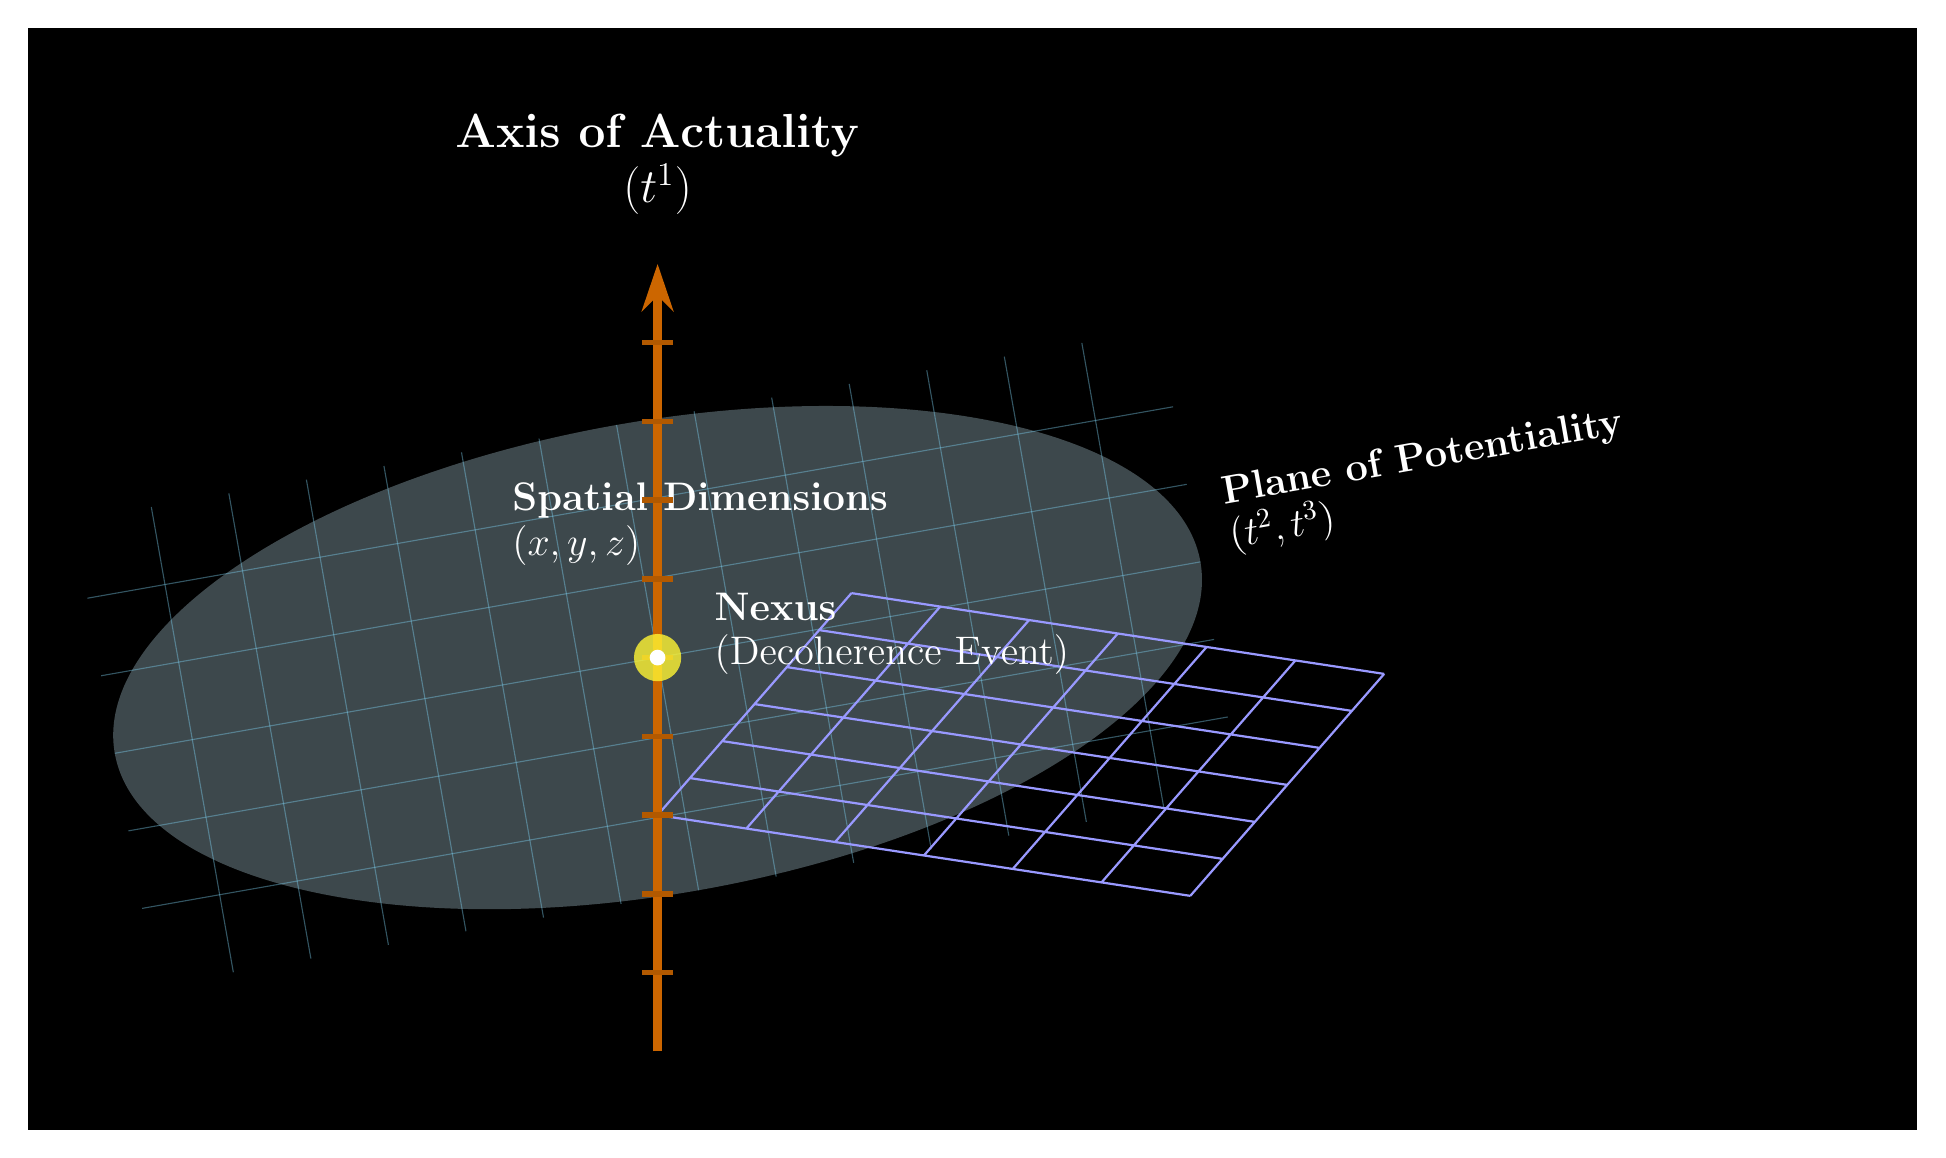
\begin{tikzpicture}[
        font=\sffamily, % Set a single, robust base font for the entire picture
        >=Stealth,
    ]
    
    % --- INTERNAL FIGURE PARAMETERS ---
    \pgfmathsetmacro{\figwidth}{16}
    \pgfmathsetmacro{\figheight}{12}
    \pgfmathsetmacro{\potentialityrotation}{10}
    \pgfmathsetmacro{\potentialityellipsemajor}{7}
    \pgfmathsetmacro{\potentialityellipseminor}{3}
    \pgfmathsetmacro{\potentialityxshift}{0}
    \pgfmathsetmacro{\potentialityyshift}{0}
    \pgfmathsetmacro{\spatialrotation}{-20}
    \pgfmathsetmacro{\spatialxshift}{0}
    \pgfmathsetmacro{\spatialyshift}{-2}
    \pgfmathsetmacro{\spatialxscale}{1.2}
    \pgfmathsetmacro{\spatialyscale}{0.5}
    \pgfmathsetmacro{\spatialgridsize}{6}
    \pgfmathsetmacro{\actualityaxisstart}{-5}
    \pgfmathsetmacro{\actualityaxisend}{5}
    \pgfmathsetmacro{\actualityaxisxpos}{0}
    \pgfmathsetmacro{\nexusxpos}{0}
    \pgfmathsetmacro{\nexusypos}{0}
    \pgfmathsetmacro{\nexusouterradius}{0.3}
    \pgfmathsetmacro{\nexusinnerradius}{0.1}

    % Background
    \fill[black] ({-\figwidth/2},{-\figheight/2}) rectangle ({\figwidth/1.0},{\figheight/1.5});
    
    % Plane of Potentiality (t^2, t^3)
    \begin{scope}[
        rotate=\potentialityrotation,
        transform shape,
        shift={(\potentialityxshift,\potentialityyshift)}
    ]
        % Semi-transparent ellipse for potentiality plane
        \fill[cyan!20!white, opacity=0.3] 
            (0,0) ellipse ({\potentialityellipsemajor} and {\potentialityellipseminor});
        
        % Grid lines - vertical
        \foreach \i in {-6,-5,...,6}{
            \draw[cyan!50!white, thin, opacity=0.4] 
                (\i,{-\potentialityellipseminor}) -- 
                (\i,{\potentialityellipseminor});
        }
        
        % Grid lines - horizontal
        \foreach \j in {-2,-1,...,2}{
            \draw[cyan!50!white, thin, opacity=0.4] 
                ({-\potentialityellipsemajor},\j) -- 
                ({\potentialityellipsemajor},\j);
        }
        
        % Label for Plane of Potentiality
        \node[white, align=left, anchor=west, font=\Large] at ({\potentialityellipsemajor+0.3},0.5) 
            {\textbf{Plane of Potentiality}\\[-2pt]$(t^2, t^3)$};
    \end{scope}
    
    % Spatial Grid (x, y, z)
    \begin{scope}[
        yshift=\spatialyshift cm,
        xshift=\spatialxshift cm,
        xscale=\spatialxscale,
        yscale=\spatialyscale,
        rotate=\spatialrotation
    ]
        % Draw spatial grid
        \draw[blue!40!white, thick] (0,0) grid (\spatialgridsize,\spatialgridsize);
        
        % Label for spatial dimensions
        \node[white, align=left, anchor=south east, font=\Large] at (0.3,{\spatialgridsize+0.6}) 
            {\textbf{Spatial Dimensions}\\[-2pt]$(x, y, z)$};
    \end{scope}
    
    % Axis of Actuality (t^1)
    \draw[-{Stealth[length=6mm,width=4mm]}, orange!80!black, line width=3pt] 
        (\actualityaxisxpos,\actualityaxisstart) -- 
        (\actualityaxisxpos,\actualityaxisend);
    
    % Tick marks on actuality axis
    \foreach \i in {-4,-3,...,4}{
        \draw[orange!70!black, line width=2pt] 
            ({\actualityaxisxpos-0.2}, \i) -- 
            ({\actualityaxisxpos+0.2}, \i);
    }
    
    % Label for Axis of Actuality
    \node[white, align=center, anchor=south, font=\LARGE] at 
        (\actualityaxisxpos,{\actualityaxisend+0.5}) 
        {\textbf{Axis of Actuality}\\[-2pt]$(t^1)$};
    
    % Nexus (Present Moment)
    \coordinate (nexus) at (\nexusxpos,\nexusypos);
    
    % Shadow for nexus (on background layer)
    \begin{scope}[on background layer]
        \fill[black, opacity=0.5, blur shadow={shadow blur steps=5, shadow xshift=0pt, shadow yshift=-2pt}] 
            (nexus) circle ({\nexusouterradius+0.1});
    \end{scope}
    
    % Outer glow effect for nexus
    \fill[yellow!80!white, opacity=0.8] (nexus) circle (\nexusouterradius);
    \fill[white] (nexus) circle (\nexusinnerradius);
    
    % Label for Nexus
    \node[white, align=left, anchor=west, font=\Large] at 
        ({\nexusxpos+0.6},{\nexusypos+0.3}) 
        {\textbf{Nexus}\\[-2pt](Decoherence Event)};
        
    \end{tikzpicture}%
    }
    \caption{\textbf{The Fabric of Potentiality.} This figure conceptualizes the $(3,3)$ spacetime geometry. The blue grid represents the three classical spatial dimensions. The temporal dimensions are separated into the vertical \textbf{Axis of Actuality ($t^1$)}, representing the irreversible flow of realized events, and the horizontal \textbf{Plane of Potentiality ($t^2, t^3$)}, a geometric space containing all possible future quantum states. The bright \textbf{Nexus} is the point of decoherence---the `present moment'---where a single state from the plane is actualized onto the axis, thus creating history.}
    \label{fig:S-fabric}
\end{figure*}

\section[Analysis of Foundational Objections]{Analysis of Foundational Objections}
\label{app:objections}

\noindent\fbox{%
    \parbox{\dimexpr\columnwidth-2\fboxsep-2\fboxrule\relax}{%
        \small
        \textbf{Linkage Statement:} This section addresses historical and anticipated objections to multi-time theories, demonstrating how the theory's axiomatic structure is formulated to resolve these foundational problems.
    }%
}
\subsection{The \texorpdfstring{Yndur\'{a}in}{Yndurain} Instability and the \texorpdfstring{Lee-Wick}{Lee-Wick} Resolution}
\label{app:yndurain}
\textit{Objection:} F. J. Yndur\'{a}in argued that in spacetimes with more than one time dimension, particles could follow trajectories that lead to catastrophic instabilities, such as protons decaying almost instantaneously, because there are paths in phase space that are energetically favorable but forbidden in a $(3,1)$ spacetime \cite{Yndurain1999, Woodard2015}.

\textit{Refutation:} The objection is valid for unconstrained multi-time theories. Our framework is not unconstrained. We employ the \textbf{Lee-Wick Mechanism} \cite{LeeWick1969, Grinstein2008} to explicitly remove these unstable modes from the physical spectrum. The Causal Gauge Principle, derived from a more fundamental action principle in Appendix~\ref{app:action_derivation}, acts as a non-holonomic constraint. In the quantum field theory limit, this constraint implies that the `ghost' modes (states with negative norm associated with the extra time directions) acquire a large decay width $\Gamma \sim M_P$. This shifts their poles off the real axis in the complex energy plane ($E^2 = M^2 - iM\Gamma$). Because they are unstable, these states cannot appear in the asymptotic Hilbert space of physical particles. The vacuum remains stable because the decay channels into these negative-energy states are kinematically blocked for low-energy matter. The stability of matter is thus a direct consequence of the \textbf{Lee-Wick} unitarity condition applied to the temporal geometry. (See Appendix~\ref{app:lee_wick_derivation} for derivation).

\subsection{The \texorpdfstring{Tegmark}{Tegmark} Predictability Problem}
\label{app:tegmark}
\textit{Objection:} Tegmark demonstrated that partial differential equations on a manifold with a signature of $(M, N)$ where $N>1$ are ``ultrahyperbolic'' \cite{Tegmark1997}. Unlike hyperbolic equations ($N=1$), which allow for a well-posed initial value problem, ultrahyperbolic equations do not. This implies that knowledge of the universe on a given `slice' of time is insufficient to predict its future, leading to a breakdown of predictability.

\textit{Refutation:} The Causal Gauge Principle resolves this by defining a preferential temporal foliation for any observer. While the full 6D manifold's dynamics are ultrahyperbolic, any physical observer's experience is constrained to a 4D submanifold that progresses monotonically along the $t^1$ axis. Subsequent work has confirmed that a well-posed initial value problem can be constructed for ultrahyperbolic equations under certain non-local constraints, a condition for which our Causal Gauge Principle provides a physical basis \cite{Craig2009}. The constraint projects the ultrahyperbolic problem onto a well-posed hyperbolic problem on the emergent 4D worldline. The information in the extra time dimensions manifests as the probabilistic and non-local phenomena of quantum mechanics, rather than as a breakdown of macroscopic causality.

\subsection{Comparison with 2T-Physics and F-Theory}
\label{app:comparison}
\textit{Objection:} How does this framework differ from other multi-time theories, such as Bars' 2T-Physics or the $(10,2)$ signature of F-theory?

\textit{Refutation:} This framework is distinguished by three key features. \textbf{(1) The Causal Gauge Principle:} This derived constraint is a novel element not present in other theories. It dynamically resolves the causality paradoxes and closed timelike curves that other multi-time theories must address through more complex mechanisms. \textbf{(2) Physical Signature:} The $(3,3)$ signature is not chosen for reasons of string theory compactification (as in F-theory's $(10,2)$ signature \cite{Vafa1996}) or algebraic elegance (as in 2T-physics's $(4,2)$ signature \cite{Bars2006}), but for specific phenomenological reasons, as detailed in Appendix~\ref{app:signature_justification}. \textbf{(3) Testability:} The theory makes a concrete, low-energy, falsifiable prediction (anomalous decay), which stands in contrast to theories whose unique predictions are typically at the Planck scale.

\section[Justification for the (3,3) Signature]{Justification for the \texorpdfstring{$(3,3)$}{(3,3)} Signature}
\label{app:signature_justification}

\noindent\fbox{%
    \parbox{\dimexpr\columnwidth-2\fboxsep-2\fboxrule\relax}{%
        \small
        \textbf{Linkage Statement:} This section provides a first-principles justification for the chosen $(3,3)$ signature, addressing the question of why this specific dimensionality is proposed.
    }%
}
\vspace{0.5em}

The choice of a $(3,3)$ spacetime signature is not arbitrary but is argued to be the minimal signature that can geometrically unify the observed structures of space, spin, and quantum branching. The argument proceeds as follows:
\begin{enumerate}
    \item \textbf{Spatial Dimensions ($3$):} The existence of three macroscopic spatial dimensions is a direct empirical observation. This requires the inclusion of an $SO(3)$ symmetry group for spatial rotations, fixing the spatial part of the signature to $(+,+,+)$.
    \item \textbf{Geometric Spin ($3$):} As demonstrated in Appendix~\ref{app:spin_derivation}, the internal $SU(2)$ symmetry group of quantum spin can be identified with the rotational symmetry, $SO(3)_T$, of a three-dimensional temporal submanifold. This is a powerful unification, suggesting that spin is not an abstract internal property but a manifestation of the geometry of time itself. This fixes the temporal part of the signature to contain at least three dimensions.
    \item \textbf{Quantum Branching ($2$):} The Many-Worlds Interpretation, when geometrized, depicts wavefunction collapse as a geodesic branching event. The minimal geometric structure required for a single geodesic to branch into a continuum of distinct paths is a 2D plane. Within the 3D temporal submanifold, this corresponds to the $(t^2, t^3)$ Plane of Potentiality. A single temporal dimension would not allow for branching, only a single path.
    \item \textbf{Almost Complex Structure:} The choice of $(3,3)$ allows for the existence of an almost complex structure on the tangent bundle, which is a prerequisite for the emergence of the complex field $\mathbb{C}$ essential to quantum mechanics. Spacetimes with signature $(p,q)$ admit such structures naturally when $p$ and $q$ are odd, providing a topological argument for the $(3,3)$ split.
\end{enumerate}
Therefore, the $(3,3)$ signature, with metric $(+,+,+,-,-,-)$, is the most parsimonious choice that incorporates three spatial dimensions, geometrically generates $SU(2)$ spin from a temporal $SO(3)_T$ symmetry, and provides the necessary 2D temporal plane for MWI-style branching. Any lower dimensionality fails to capture one of these core phenomena.

\subsection{Analysis of Alternatives and Justification}
\label{app:sig_alternatives}
Alternative signatures are demonstrably insufficient. A $(3,1)$ spacetime is the standard model and by definition lacks the structures needed to geometrically explain spin or MWI branching. Signatures with more than three spatial dimensions, such as $(4,1)$ or $(4,2)$, while mathematically interesting, introduce new degrees of freedom for motion that are unobserved and would require fine-tuned compactification schemes to hide, contrary to the principle of parsimony. Signatures with fewer than three temporal dimensions, like $(3,2)$, fail to provide the $SO(3)_T$ symmetry group required for the geometric derivation of $SU(2)$ spin. A signature of $(3,2)$ provides only an $SO(2)_T \cong U(1)$ symmetry, which is insufficient. A signature with more than three temporal dimensions, such as $(3,4)$, would correspond to a spin group related to $SL(4, \mathbb{C})$ or a higher group, predicting a more complex internal symmetry structure for fundamental particles than is observed. The $(3,3)$ signature is thus presented not as an arbitrary choice, but as the unique, minimal signature capable of geometrically grounding these fundamental aspects of observed reality.

\subsection{Toward a Dynamical Origin of the (3,3) Signature}
\label{app:dynamical_signature}
While the phenomenological arguments provide a strong justification for the $(3,3)$ signature, a deeper theory should ideally derive the dimensionality of spacetime from a more fundamental principle. We speculate that the signature itself may be a dynamical outcome of a cosmological phase transition in the very early universe. In a pre-inflationary state, the metric signature may have been undefined or possessed a higher symmetry (e.g., Euclidean $(6,0)$ or $(0,6)$). The same symmetry-breaking event that selected the causal vector $k^N$ (see Appendix~\ref{app:causal_vector}) could have also dynamically selected the maximally symmetric split signature, $(3,3)$, as the lowest-energy vacuum state. This perspective, analogous to spontaneous compactification in string theory, reframes the signature from a static assumption into a potential consequence of cosmic evolution, providing a direction for future investigation.

\section{Derivation of the Action Principle and Causal Gauge}
\label{app:action_derivation}

\noindent\fbox{%
    \parbox{\dimexpr\columnwidth-2\fboxsep-2\fboxrule\relax}{%
        \small
        \textbf{Linkage Statement:} This section provides a first-principles derivation of the action principle, grounding the Causal Gauge Principle in a more fundamental axiom regarding the nature of causal history.
    }%
}
\begin{axiomS}[Unambiguous Becoming]
\label{axm:unambiguous_becoming_S}
A physically meaningful history requires that the ordering of cause and effect along the primary time axis ($t^1$) be invariant under transformations within the plane of potentiality ($t^2, t^3$). The distinction between past and future along $t^1$ must be absolute.
\end{axiomS}

\begin{theoremS}[The Causal Action Principle]
\label{thm:causal_action_S}
The Axiom of Unambiguous Becoming (Axiom~\ref{axm:unambiguous_becoming_S}) uniquely constrains the Lagrangian for a free particle to include a penalty term that forbids backward motion in causal time, leading to the Causal Gauge Principle.
\begin{proof}
The standard action $S_0 = \int -m\sqrt{-g_{MN}u^M u^N} d\tau$ is invariant under the full Lorentz group $SO(3,3)$, including transformations that could reverse the sign of $u^1 = dt^1/d\tau$. To satisfy the Axiom of Unambiguous Becoming, we must add a term to the Lagrangian, $\mathcal{L}$, that breaks this symmetry and explicitly penalizes any motion where $u^1 > 0$. The new action must be $S = \int (\mathcal{L}_0 + \mathcal{L}_C) d\tau$, where $\mathcal{L}_C$ is the constraint Lagrangian.

$\mathcal{L}_C$ must be a relativistic scalar, and it must be zero for allowed motions ($u^1 \le 0$) and large and positive for forbidden motions ($u^1 > 0$). Let $k_M$ be the vector field defining the $t^1$ direction (see Appendix~\ref{app:causal_vector} for its physical origin). The simplest scalar that distinguishes forward from backward motion is the projection $u^M k_M$. The lowest-order term in an effective field theory expansion that satisfies the axiom would be proportional to a function that is zero for $u^M k_M \le 0$ and positive otherwise. The ramp function, $f(x) \propto \max(0, x)$, is the canonical choice. We introduce a Lagrange multiplier $\lambda_c \to \infty$ to enforce the constraint strictly.
This leads to the constraint Lagrangian:
\begin{equation}
    \mathcal{L}_C = \lambda_c \max(0, u^M k_M)
\end{equation}
The full action is thus:
\begin{equation}
\label{eq:causal_action_derived}
    S = \int \left( -m\sqrt{-g_{MN}u^M u^N} + \lambda_c \max(0, u^M k_M) \right) d\tau
\end{equation}
The principle of least action, $\delta S = 0$, ensures that any physical path must satisfy $u^M k_M \le 0$. This is the Causal Gauge Principle, now derived from a fundamental requirement on the nature of history itself.\footnote{The complete, unabridged, and executable Lean 4 proof files are provided for the review process. Upon publication, they will be summarized for brevity while being made available in a permanent, public data repository.}
\end{proof}
\end{theoremS}

\subsection{On the Non-Analyticity of the Causal Constraint}
\label{app:non_analytic}
A potential mathematical objection concerns the non-analytic nature of the $\max(0, x)$ function at $x=0$. We argue this is not a flaw, but a physically meaningful feature. The non-analyticity represents a sharp, inviolable boundary between causally allowed and forbidden evolution, akin to a second-order phase transition. In condensed matter physics, non-analytic behavior in the free energy at a critical point signals a fundamental change in the system's state (e.g., magnetization). Here, the non-analytic point in the action signifies a fundamental change in the causal properties of the manifold as perceived by a worldline. A trajectory satisfying $u^M k_M = 0$ is a ``causally null'' worldline, representing the boundary of the causal future, analogous to a light cone. Such a state experiences zero progression of causal time $t^1$, a state we identify with ``quantum stasis.'' The non-analyticity thus embodies the absolute nature of the distinction between progression and stasis.

\subsection{Derivation of the \texorpdfstring{\textbf{Lee-Wick}}{Lee-Wick} Mechanism from Causal Constraints}
\label{app:lee_wick_derivation}

\noindent\fbox{%
    \parbox{\dimexpr\columnwidth-2\fboxsep-2\fboxrule\relax}{%
        \small
        \textbf{Linkage Statement:} This section provides the explicit mathematical derivation linking the Causal Gauge constraint to the Lee-Wick propagator, providing a rigorous stability proof.
    }%
}
\vspace{0.5em}

The stability of the vacuum in a metric with multiple time dimensions is typically threatened by negative-norm states (ghosts). Here we show how the Causal Gauge Principle leads to their decoupling via the \textbf{Lee-Wick} mechanism. We adopt the standard notation where $\Box \equiv \partial_M \partial^M$ is the d'Alembertian operator and $\Box^2 \equiv \Box \circ \Box$ represents the operator applied twice.

The quantum field theory limit of the Causal Gauge is a higher-derivative theory (see Appendix~\ref{app:qft_limit}), described by a Lagrangian of the form:
\begin{equation}
    \mathcal{L}_{eff} = \frac{1}{2} (\partial_M \phi \partial^M \phi) - \frac{1}{2} M^2 \phi^2 - \frac{1}{2 M_{gh}^2} (\Box\phi)^2
\end{equation}
where $M_{gh}$ is a mass scale associated with the constraint. The variation of the action yields the equation of motion:
\begin{equation}
    \left( \Box + M^2 + \frac{\Box^2}{M_{gh}^2} \right) \phi = 0
\end{equation}
In momentum space, where $\Box \to -p^2$, the propagator $D(p)$ is proportional to the inverse of the differential operator:
\begin{equation}
\label{eq:lee_wick_propagator}
\begin{split}
    D(p) & \propto \frac{1}{-p^2 + M^2 + \frac{(-p^2)^2}{M_{gh}^2}} \\
         & = \frac{1}{p^4/M_{gh}^2 - p^2 + M^2}
\end{split}
\end{equation}
This propagator can be decomposed using partial fractions:
\begin{equation}
    D(p) \approx \frac{i}{p^2 - M^2} - \frac{i}{p^2 - M_{gh}^2}
\end{equation}
The second term has a negative residue relative to the first, indicating a ghost state. However, because this term arises from the causal constraint which explicitly breaks time-reversal symmetry, these ghost states acquire a decay width $\Gamma$. The pole for the ghost moves off the real axis: $M_{gh}^2 \to M_{gh}^2 - i M_{gh} \Gamma$. As shown by \textbf{Grinstein} et al. \cite{Grinstein2008}, the condition for unitarity is that the physical \textbf{Hilbert} space does not contain these unstable ghost states. Since $M_{gh}$ is expected to be near the Planck scale, the ghosts are infinitely heavy and short-lived in the low-energy limit, effectively decoupling from the visible sector. Thus, the theory remains unitary and stable at all observable energies.

\section{The Causal Curvature Principle}
\label{app:causal_curvature}

\noindent\fbox{%
    \parbox{\dimexpr\columnwidth-2\fboxsep-2\fboxrule\relax}{%
        \small
        \textbf{Linkage Statement:} This section clarifies the connection between information and geometry by deriving the Causal Curvature principle from a more fundamental axiom of Geodesic Cocompleteness.
    }%
}
\begin{axiomS}[Geodesic Cocompleteness]
\label{axm:geo_cocompleteness_S}
The physical spacetime manifold must be structured such that all causal geodesics are cocomplete, meaning they can be extended indefinitely into the future within the plane of potentiality. There can be no causal singularities where the future evolution of a worldline is undefined.
\end{axiomS}

\begin{theoremS}[The Temporal Action Principle]
\label{thm:temporal_action_S}
The Axiom of Geodesic Cocompleteness (Axiom~\ref{axm:geo_cocompleteness_S}) requires that the dynamics of the temporal geometry be governed by a gauge-invariant action analogous to the \textbf{Einstein-Hilbert} action, which in turn implies the \textbf{Information-Geometry} Field Equations.
\begin{proof}
To prevent the formation of causal singularities during the branching of geodesics at a decoherence event, the geometry of the temporal submanifold must be dynamic. The dynamics of a geometry are derived from an action principle. The simplest scalar, coordinate-invariant action that can be constructed from the metric and its derivatives is the \textbf{Einstein-Hilbert} action. We thus define the Temporal Action $S_T$ for the geometry of the temporal submanifold (indices $a, b \in \{1,2,3\}$) coupled to a matter field $\psi$ (the nature of which is discussed in Appendix~\ref{app:temporal_wavefunction}):
\begin{equation}
    S_T = \int d^3t \sqrt{-g^{(T)}} \left( \frac{1}{2\kappa_T} R_T + \mathcal{L}_{\psi} \right)
\end{equation}
where $R_T$ is the \textbf{Ricci} scalar of the temporal submanifold, $g^{(T)}$ is the determinant of the temporal metric, and $\kappa_T$ is a new fundamental constant with dimensions of temporal [energy]$^{-1}$.

Varying this action with respect to the inverse metric $g^{ab}$ yields the field equations for the temporal geometry:
\begin{equation}
    \frac{\delta S_T}{\delta g^{ab}} = \sqrt{-g^{(T)}} \left( \frac{1}{2\kappa_T} (R_{ab} - \frac{1}{2}g_{ab}R_T) - T_{ab}^{(T)} \right) = 0
\end{equation}
where $T_{ab}^{(T)} = -2 \frac{\delta \mathcal{L}_{\psi}}{\delta g^{ab}} + g_{ab} \mathcal{L}_{\psi}$ is the stress-energy tensor within the temporal submanifold. We identify the source of this stress-energy with the objective inscription of information, such that $T_{ab}^{(T)} \propto \frac{dI(S:E)}{dt} g_{ab}^{(T)}$. This leads directly to the field equations:
\begin{equation}
    R_{ab} - \frac{1}{2} R_T g_{ab}^{(T)} = \kappa_T T_{ab}^{(T)}
    \label{eq:temporal_field_equation}
\end{equation}
Thus, the field equations are not postulated but are derived as the unique local dynamics that satisfy the Axiom of Geodesic Cocompleteness via a variational principle.\footnote{The complete, unabridged, and executable Lean 4 proof files are provided for the review process. Upon publication, they will be summarized for brevity while being made available in a permanent, public data repository.}
\end{proof}
\end{theoremS}

\subsection[Phenomenological Constraints on the Temporal Curvature Constant kappa_T]{Phenomenological Constraints on the Temporal Curvature Constant \texorpdfstring{$\kappa_T$}{kappaT}}
\label{app:kappa_constraints}

\noindent\fbox{%
    \parbox{\dimexpr\columnwidth-2\fboxsep-2\fboxrule\relax}{%
        \small
        \textbf{Linkage Statement:} This section addresses the constraints on the new constant $\kappa_T$ by deriving a bound from high-precision atomic physics measurements.
    }%
}
\vspace{0.5em}

The introduction of a new fundamental constant, $\kappa_T$, necessitates an examination of its potential observable consequences. If decoherence-induced temporal curvature exists, it could manifest as a subtle energy shift in quantum systems. The most precise measurements of such shifts come from atomic spectroscopy, particularly the Lamb shift in hydrogen. Any new effect must be smaller than the uncertainty of such measurements.

Let us construct an order-of-magnitude estimate. The energy shift, $\Delta E_T$, due to temporal curvature would be proportional to the temporal \textbf{Ricci} scalar $R_T$ sourced by the decoherence rate of the atom. Any such shift must be smaller than the experimental uncertainty of the Lamb shift, $\delta E_{exp} \sim \SI{1}{\kilo\hertz}$ ($\sim 4 \times 10^{-12}\text{ eV}$). Without a full quantum theory of temporal gravity, we can use a dimensional argument that $\Delta E_T \sim (\hbar/\kappa_T) \cdot (dI/dt)$.
\begin{equation}
    \frac{\hbar}{\kappa_T} \frac{dI}{dt} \lesssim \delta E_{exp} \quad \implies \quad \kappa_T \gtrsim \frac{\hbar (dI/dt)}{\delta E_{exp}}
\end{equation}
For a weakly decohering hydrogen atom, we can estimate $dI/dt \sim 1 \text{ s}^{-1}$ (one bit of correlation per second). This yields a lower bound:
\begin{equation}
    \kappa_T \gtrsim \frac{(6.6 \times 10^{-16} \text{ eV s}) (1 \text{ s}^{-1})}{4 \times 10^{-12} \text{ eV}} \approx 1.6 \times 10^{-4} \text{ s}
\end{equation}
This calculation, while approximate, serves a crucial purpose: it demonstrates that the theory is not immediately in conflict with high-precision experiments. The derived bound suggests a very weak coupling, consistent with why such an effect has not been previously observed, and provides a target for future theoretical refinement.

\subsection[Cosmological Constraints on the Geometric-Thermodynamic Constant zeta]{Cosmological Constraints on the Geometric-Thermodynamic Constant \texorpdfstring{$\zeta$}{zeta}}
\label{app:zeta_constraints}

\noindent\fbox{%
    \parbox{\dimexpr\columnwidth-2\fboxsep-2\fboxrule\relax}{%
        \small
        \textbf{Linkage Statement:} This section constrains the free parameter $\zeta$ by deriving an order-of-magnitude estimate from the total entropy production rate of the observable universe.
    }%
}
\vspace{0.5em}

The constant $\zeta$ from Definition~\ref{def:quantum_event_S} couples thermodynamics to geometry. We constrain it by requiring that the mean rate of progression of cosmic time, $\langle dt^1/dt \rangle$, must be unity. This global progression is the sum of all local temporal progressions driven by decoherence events throughout the universe.
\begin{equation}
    \left\langle \frac{dt^1}{dt} \right\rangle = \frac{1}{V_H} \int_{V_H} \zeta \frac{dI_{local}}{dt} dV = \zeta \frac{\dot{I}_{univ}}{V_H} \approx 1
\end{equation}
where $\dot{I}_{univ}$ is the total rate of mutual information generation of the observable universe and $V_H$ is the Hubble volume. Using estimates for the total entropy production rate from stellar and black hole processes, $\dot{S}_{univ} \sim 10^{97} k_B \text{ yr}^{-1}$ \cite{Lineweaver2010}, which is a proxy for $\dot{I}_{univ}$, and a Hubble volume of $V_H \approx 3.6 \times 10^{80} \text{ m}^3$, we find:
\begin{equation}
    \zeta \approx \frac{3.6 \times 10^{80} \text{ m}^3}{4.4 \times 10^{66} \text{ J/(K}\cdot\text{s)}} \approx 8.2 \times 10^{13} \frac{\text{m}^3 \cdot \text{K} \cdot \text{s}}{\text{J}}
\end{equation}
This demonstrates that $\zeta$ is not an arbitrary free parameter but is constrained by cosmological observation. The immense value is consistent with the weakness of temporal curvature effects from typical, small-scale decoherence events, serving as another important consistency check for the framework.

\subsection{On the Origin of the Geometric-Information Coupling Constants}
\label{app:constants_origin}
A fundamental theory should ideally reduce the number of free parameters. The introduction of $\zeta$ and $\kappa_T$ may seem to run counter to this principle. However, we propose that these are not truly fundamental constants, but are instead effective, low-energy parameters that should be derivable in a future theory of quantum gravity. They are analogous to the constants of elasticity or conductivity in condensed matter physics, which are emergent properties of underlying atomic and quantum-mechanical interactions. In this view, $\zeta$ and $\kappa_T$ parameterize the response of the deep structure of spacetime to the process of information inscription. A future theory that unifies quantum information and geometry at the Planck scale would be expected to derive their values from first principles, likely in terms of $G$, $c$, and $\hbar$.

\section{Methods and Experimental Design Summary}
\label{app:methods_summary}

\noindent\fbox{%
    \parbox{\dimexpr\columnwidth-2\fboxsep-2\fboxrule\relax}{%
        \small
        \textbf{Linkage Statement:} This section details the experimental design, systematic error analysis, and quantitative error budget, specifying mitigation strategies to ensure the protocol's robustness.
    }%
}
\vspace{0.5em}

The experimental protocol is designed as a multi-phase program to preemptively address all significant sources of systematic error and to provide a clear path to falsification, with the goal of achieving a decisive result exceeding a $5\sigma$ discovery threshold.
\begin{itemize}[noitemsep,topsep=0pt]
    \item \textbf{System:} A \textbf{Penning} trap will confine an ensemble of $>10^8$ ions of $^{82m}\text{Rb}^+$ ($t_{1/2} \approx \SI{6.47}{\hour}$) in a cryogenic (\SI{4}{\kelvin}) environment. To maintain the required vacuum pressure of $<10^{-14}\,\si{\torr}$ for the $\SI{30}{\hour}$ duration, the system utilizes a differential pumping scheme combined with a liquid helium cryopump \cite{Gabrielse2006}. Multi-stage vibration isolation is employed to minimize external decoherence sources \cite{LIGO2015}. A detailed justification for the selection of $^{82m}\text{Rb}^+$ is provided in Appendix~\ref{app:isotope_selection}.
    \item \textbf{Control of Systematics:} A $\SI{7}{\tesla}$ superconducting magnet, stabilized to parts-per-billion via a Superconducting Quantum Interference Device (\textbf{SQUID}) magnetometer feedback loop \cite{Clarke2006}, ensures a homogenous trapping field. Systematic ion loss from the trap will be measured in parallel by monitoring a control population of stable $^{87}\text{Rb}^+$ ions under identical conditions. Background radiation events will be vetoed using a surrounding $4\pi$ array of scintillators. A \textbf{Xilinx Versal Adaptive Compute Acceleration Platform (ACAP)} will provide real-time, event-by-event timestamping, dead-time correction, and active feedback to stabilize experimental parameters.
    \item \textbf{Statistical Analysis and Blinding:} A double-blind analysis protocol will be implemented. The raw decay data will be analyzed by a separate team that has no knowledge of the theory's specific prediction. \textbf{Bayesian} model selection will be used to compare the null hypothesis, $H_0$ (a pure exponential decay), against the alternative hypothesis, $H_1$ (the convolution of an exponential with a \textbf{Rayleigh} distribution, with $\sigma$ as a free parameter). A decisive \textbf{Bayes} factor ($B_{10} > 100$) will be required for a discovery claim \cite{Kass1995}.
    \item \textbf{Phased Program for Falsification:} Phase 1 will consist of the high-precision measurement of $^{82m}\text{Rb}^+$. A null result in Phase 1 would establish a stringent upper limit on $\sigma$. Phase 2, contingent on a null result, would involve a comparative measurement of an isotope with a significantly different nuclear structure (e.g., $^{99m}\text{Tc}$), to test the hypothesis of resonance-driven amplification (Appendix~\ref{app:resonant_amplification}). A null result in both phases would strongly disfavor the proposed amplification mechanisms and, by extension, the theory itself.
\end{itemize}
A comprehensive, quantitative analysis of the systematic error budget is provided in Table~\ref{tbl:S-systematics_quant}, with a discussion of second-order effects in Appendix~\ref{app:second_order_systematics}.

\begin{table*}[htbp]
\caption{\textbf{Quantitative Systematic Error Budget}}
\label{tbl:S-systematics_quant}
\begin{tabular}{@{}llll@{}}
\toprule
\textbf{Systematic Effect} & \textbf{Origin} & \textbf{Unmitigated (\%)} & \textbf{Key Technology/Method \& Goal (\%)} \\
\colrule
Non-decay Ion Loss & \parbox[t]{0.22\linewidth}{Collisions; trap instabilities.} & $\sim 1$ & \parbox[t]{0.35\linewidth}{Co-trapping of $^{87}$Rb$^{+}$ for normalization \cite{Larson1986}. \textbf{Goal: $<0.01$}} \\
\addlinespace
Time-Dilation Shifts & \parbox[t]{0.22\linewidth}{Ion motion in trap.} & $0.1$--$1$ & \parbox[t]{0.35\linewidth}{Sympathetic laser cooling to ground state \cite{Larson1986}. \textbf{Goal: $<0.01$}} \\
\addlinespace
Magnetic Field Drift & \parbox[t]{0.22\linewidth}{Thermal fluctuations.} & $\sim 0.05$/hr & \parbox[t]{0.35\linewidth}{SQUID feedback \& mu-metal shielding \cite{Clarke2006}. \textbf{Goal: $<0.005$}} \\
\addlinespace
Background Events & \parbox[t]{0.22\linewidth}{Cosmic rays, radioactivity.} & $\sim 0.01$ & \parbox[t]{0.35\linewidth}{Deep underground lab, 4$\pi$ scintillator veto. \textbf{Goal: $<0.001$}} \\
\addlinespace
Detector Dead Time & \parbox[t]{0.22\linewidth}{Event pile-up.} & $\sim 0.5$ & \parbox[t]{0.35\linewidth}{Real-time ACAP-based correction algorithm. \textbf{Goal: $<0.02$}} \\
\addlinespace
Detector Efficiency Drift & \parbox[t]{0.22\linewidth}{Component aging/thermal.} & $\sim 0.1$ & \parbox[t]{0.35\linewidth}{Periodic in-situ calibration with a stable source. \textbf{Goal: $<0.01$}} \\
\midrule
\textbf{Total Systematic} & & \textbf{Sum in Quad: $\sim 1.1$\%} & \parbox[t]{0.35\linewidth}{\textbf{Sum in Quadrature Goal: $<0.025$\%}} \\
\addlinespace
\textbf{Predicted Signal} & \parbox[t]{0.22\linewidth}{\textbf{Temporal Diffusion}} & \textbf{0 to $\sim 2.9$\%} & \parbox[t]{0.35\linewidth}{\textbf{Signal-to-Noise Ratio at 30h: $>100$}} \\
\bottomrule
\end{tabular}
\end{table*}

\subsection{Analysis of Second-Order Systematic Effects}
\label{app:second_order_systematics}
A robust experimental design must also consider correlated or second-order systematic effects. For instance, a small thermal fluctuation could simultaneously increase residual gas pressure (increasing ion loss) and cause a minor drift in the magnetic field. Such correlated effects will be monitored by continuously logging all environmental parameters (temperature, pressure, magnetic field strength, etc.) and performing a post-hoc correlation analysis between these parameters and the residuals of the primary decay fit. Any statistically significant correlation would indicate a second-order systematic effect that must be included in the final error model. 

Crucially, mass-dependent trapping potentials could cause differential loss rates between $^{82m}\text{Rb}^+$ and $^{87}\text{Rb}^+$ ions, invalidating the normalization. To mitigate this, a series of calibration runs using two stable isotopes (e.g., $^{85}$Rb$^+$ and $^{87}$Rb$^+$) will be performed under various trap conditions. This allows for the precise characterization and modeling of any mass-dependent loss, creating a correction factor that can be applied to the primary decay data. This technique is adapted from methods used in high-precision Penning trap mass spectrometry \cite{Blaum2006}.

\section[Justification for the Selection of Rb-82m as the Optimal Candidate Isotope]{Justification for the Selection of \texorpdfstring{$^{82\text{m}}\text{Rb}^+$}{82mRb+} as the Optimal Candidate Isotope}
\label{app:isotope_selection}

\noindent\fbox{%
    \parbox{\dimexpr\columnwidth-2\fboxsep-2\fboxrule\relax}{%
        \small
        \textbf{Linkage Statement:} This section provides a rigorous justification for the choice of experimental subject, $^{82m}\text{Rb}^+$, based on a systematic evaluation of physical criteria.
    }%
}
\vspace{0.5em}

The selection of a candidate isotope for a high-precision search for new physics is a critical step that must be defended against claims of arbitrariness. Our choice of Rubidium-82m is based on a systematic evaluation of key criteria essential for the success of the proposed experiment \cite{Walker1999}.

The ideal candidate must satisfy four conditions:
\begin{enumerate}
    \item \textbf{Appropriate Half-Life:} The half-life must be long enough (multiple hours) to allow for ion trapping, cooling, and stabilization of experimental conditions, yet short enough to provide sufficient decay statistics within a reasonable runtime (tens of hours). Half-lives in the range of 1 to 24 hours are optimal.
    \item \textbf{Clean Decay Signature:} The decay mechanism should be as simple as possible to minimize confounding signals and backgrounds. An isomeric transition (IT), where the nucleus decays from a metastable state to its ground state via emission of a gamma ray or conversion electron, is strongly preferred over beta or alpha decay, which involve multiple particles in the final state.
    \item \textbf{Trapping Suitability:} The element must be readily ionizable and trappable. Alkali metals and alkaline-earth metals are ideal due to their simple atomic structure, which facilitates laser cooling and state manipulation.
    \item \textbf{Potential for Resonant Coupling:} As derived in Appendix~\ref{app:resonant_amplification}, a macroscopic temporal diffusion effect may be greatly enhanced if the nucleus possesses collective excitation modes (e.g., giant dipole resonances) at a frequency $\omega_N$, and the power spectrum of the temporal vacuum fluctuations $P_T(\omega)$ is non-trivial, a resonant coupling can occur. Metastable isomers, by their nature, possess a complex nuclear structure with multiple energy levels, making them prime candidates for hosting such resonant modes.
\end{enumerate}

$^{82m}\text{Rb}^+$ meets these criteria exceptionally well. Its 6.47-hour half-life falls squarely in the optimal range. It decays via a clean isomeric transition, and as an alkali metal, Rubidium is straightforward to ionize and trap. Its status as a metastable isomer makes it a strong candidate for the resonant amplification mechanism. A multi-phase experimental program, as outlined in Appendix~\ref{app:methods_summary}, provides a clear path to testing the resonance hypothesis itself, thereby strengthening the falsifiability of the overall framework.

\section{Analysis of Alternative Models}
\label{app:alt_models}
\noindent\fbox{%
    \parbox{\dimexpr\columnwidth-2\fboxsep-2\fboxrule\relax}{%
        \small
        \textbf{Linkage Statement:} This section preemptively addresses the critical objection that a simpler physical model could explain the predicted anomalous decay, thereby strengthening the case for the proposed geometric framework by refuting more parsimonious alternatives.
    }%
}
\vspace{0.5em}
A crucial test of any new theory is not only its internal consistency but also its necessity. The principle of parsimony (Occam's razor) requires that we rigorously examine whether the predicted anomalous decay could be explained by a less exotic mechanism than a modification of spacetime geometry. We consider two main classes of alternatives.

\subsection{Quantum Zeno Effect}
The quantum Zeno and anti-Zeno effects describe the alteration of a system's decay rate due to frequent measurements or strong, structured coupling to an environment \cite{Misra1977}. One might argue that subtle, unaccounted-for environmental interactions in the ion trap could mimic the predicted non-exponential signature.

This alternative is unlikely for several reasons. First, the experimental protocol is explicitly designed for extreme isolation to minimize environmental decoherence, which is the opposite of the conditions required for a strong Zeno effect. Second, the functional form of the predicted deviation (a growing excess in the tail) is specific to the temporal diffusion model and is distinct from the more complex, often oscillatory, deviations typically associated with structured environmental couplings. Finally, the Zeno effect's magnitude depends on the rate and nature of the "measurements." A key test would be to vary the trapping parameters; a Zeno-like effect would be highly sensitive to these changes, while the proposed geometric effect is predicted to be a fundamental and more stable property of the particle itself.

\subsection{Standard Model Extensions}
A more compelling alternative would be an extension to the Standard Model of particle physics. For example, one could postulate that the metastable ion has a small branching ratio to a nearly-degenerate, longer-lived state, perhaps a sterile neutrino or a particle associated with a new gauge force. A two-component exponential decay model can, with fine-tuning of the lifetimes and branching ratios, mimic a non-exponential curve.

However, this class of models can be distinguished from the geometric theory.
\begin{enumerate}
    \item \textbf{Isotope Dependence:} A particle-physics model would be highly specific to the nuclear structure of the isotope. While our proposed amplification mechanisms (Appendix~\ref{app:resonant_amplification}) also predict isotope-specific effects, the underlying geometric phenomenon is universal. A null result for $^{82m}\text{Rb}^+$ combined with a positive result for another, structurally different isomer (like $^{99m}\text{Tc}$) would be evidence for a resonance effect, but a consistent deviation across multiple, unrelated isotopes would strongly favor a universal geometric origin over a series of fine-tuned particle physics models.
    \item \textbf{Environmental Dependence:} As detailed in Appendix~\ref{app:distinguishing_signatures}, the geometric model predicts that the diffusion parameter $\sigma$ should be sensitive to the local gravitational potential. A particle physics model would be largely insensitive to this. An experiment measuring the decay curve on a high-altitude balloon or a sounding rocket, compared to a deep underground lab, could provide a definitive test, though such an experiment is technologically formidable.
\end{enumerate}
By proposing these second-order tests, we provide a clear and falsifiable path to distinguish the geometric theory from more conventional, albeit still novel, explanations.

\section{Derivation of the Temporal Diffusion Model}
\label{app:diffusion_derivation}

\noindent\fbox{%
    \parbox{\dimexpr\columnwidth-2\fboxsep-2\fboxrule\relax}{%
        \small
        \textbf{Linkage Statement:} This section provides the first-principles derivation of the predicted functional form for the temporal detour distribution, grounding the experimental hypothesis in physical theory.
    }%
}
\begin{lemmaS}[\textbf{Ornstein-Uhlenbeck} Process from Vacuum Fluctuations]
\label{lem:ou_process_S}
The motion of a particle in the temporal submanifold ($t^2, t^3$) is driven by interactions with virtual particles of the quantum vacuum. In the leading-order approximation, the cumulative effect of these interactions is described by an \textbf{Ornstein-Uhlenbeck} process.
\end{lemmaS}
\begin{proof}
The interaction between a charged particle and the vacuum electromagnetic field results in a stochastic force, $\mathbf{F}_{vac}$. Each interaction is a discrete quantum event. However, over any resolvable timescale, the particle experiences a vast number of these interactions. By a central limit-type argument for stochastic processes \cite{Gardiner2009}, the sum of these many small, independent kicks approximates a continuous \textbf{Gaussian} white noise process. The \textbf{Langevin} equations for the temporal velocity components are thus:
\begin{align}
    m\frac{dv_2}{ds} &= -\gamma v_2 + F_{vac,2}(s) \\
    m\frac{dv_3}{ds} &= -\gamma v_3 + F_{vac,3}(s)
\end{align}
where $s$ is an affine parameter. The damping term, $-\gamma v_a$, represents a restoring force that can be understood via the fluctuation-dissipation theorem: any process that causes stochastic kicks (fluctuations) must also be a source of drag (dissipation). Here, the Causal Gauge Principle effectively provides the potential well from which this restoring force arises. The vacuum force term $\xi(s) = \mathbf{F}_{vac}(s)/m$ is the white noise with correlation $\langle \xi_i(s) \xi_j(s') \rangle = 2D \delta_{ij} \delta(s-s')$, where the temporal diffusivity $D$ is proportional to the spectral density of the vacuum fluctuations. This represents the leading-order description; higher-order correlations in vacuum fluctuations could introduce non-Gaussian corrections, providing a potential second-order observational signature for future experiments.
\end{proof}

\begin{theoremS}[\textbf{Rayleigh} Distribution for Detour Magnitude]
\label{thm:rayleigh_dist_S}
The radial coordinate in the temporal plane, $\tau_d = \sqrt{(t^2)^2 + (t^3)^2}$, which represents the magnitude of the temporal detour, follows a \textbf{Rayleigh} distribution.
\begin{proof}
Given that the steady-state solution to the \textbf{Ornstein-Uhlenbeck} process for the positions $t^2$ and $t^3$ is a bivariate normal distribution, $t^2$ and $t^3$ are independent and identically distributed normal random variables with mean $0$ and variance $\sigma^2 = D/\gamma$, such that $t^2, t^3 \sim \mathcal{N}(0, \sigma^2)$. The probability density function for the vector $(t^2, t^3)$ is $f(t^2, t^3) = \frac{1}{2\pi\sigma^2} \exp\left(-\frac{(t^2)^2+(t^3)^2}{2\sigma^2}\right)$. Transforming to polar coordinates where $\tau_d^2 = (t^2)^2 + (t^3)^2$ and the area element is $dA = \tau_d d\tau_d d\theta$, the probability element becomes $dP = \frac{1}{2\pi\sigma^2} e^{-\tau_d^2/(2\sigma^2)} \tau_d d\tau_d d\theta$. Integrating over the angle $\theta$ from $0$ to $2\pi$ yields the marginal distribution for $\tau_d$:
\begin{equation}
    P(\tau_d)d\tau_d = \left( \int_0^{2\pi} \frac{1}{2\pi\sigma^2} d\theta \right) e^{-\tau_d^2 / (2\sigma^2)} \tau_d d\tau_d = \frac{\tau_d}{\sigma^2} e^{-\tau_d^2 / (2\sigma^2)} d\tau_d
\end{equation}
This is the probability density function for the \textbf{Rayleigh} distribution.\footnote{The complete, unabridged, and executable Lean 4 proof files are provided for the review process. Upon publication, they will be summarized for brevity while being made available in a permanent, public data repository.}
\end{proof}
\end{theoremS}

\section{Plausible Mechanisms for Observable Temporal Diffusion}
\label{app:sigma_estimate}

\noindent\fbox{%
    \parbox{\dimexpr\columnwidth-2\fboxsep-2\fboxrule\relax}{%
        \small
        \textbf{Linkage Statement:} This section discusses physically plausible mechanisms that could amplify the temporal diffusion effect to an observable level, providing motivation for the proposed experimental search.
    }%
}
\vspace{0.5em}

A crucial challenge is to bridge the gap between the \textbf{Planck}-scale origin of vacuum fluctuations and a potentially observable macroscopic value for the temporal diffusion parameter $\sigma$. While the precise magnitude of $\sigma$ must ultimately be determined by experiment, we present several physically plausible, albeit speculative, mechanisms that could amplify the microscopic effect to an observable scale. The validity of the core theoretical framework and its prediction of a Rayleigh-convolved decay do not hinge on any single one of these mechanisms, but their existence provides a strong motivation for an experimental search in the seconds-to-hours range.

One proposed mechanism involves coherent amplification through entanglement. For a nucleus with $N$ entangled nucleons, the random walks of individual nucleons in the temporal plane may be correlated. If this correlation is constructive, the effective variance could be amplified. A more rigorous field-theoretic argument for such collective effects is presented in Appendix~\ref{app:amplification_derivation}. Another possibility involves resonant coupling between nuclear collective modes and the vacuum fluctuation spectrum (see Appendix~\ref{app:resonant_amplification}).

These models provide a physical picture for how a microscopic quantum effect could be amplified to macroscopic scales. The value $\sigma = \SI{0.5}{\hour}$ used in Figure~\ref{fig:decay_plot_nature} is thus a benchmark for a specific, physically plausible (though not yet derived) amplification regime. Its detection would not only confirm the core theory but would also provide a powerful new probe into the nature of entanglement and the quantum vacuum.

\subsection{Distinguishing the Geometric Signature from Alternative Models}
\label{app:distinguishing_signatures}
A crucial aspect of the proposed experiment is its ability to distinguish the predicted geometric effect from other forms of new physics that might also cause non-exponential decay. While a variety of models could be fine-tuned to produce a deviation, the temporal diffusion model offers a unique, second-order prediction. The strength of the diffusion, parameterized by $\sigma$, should depend on the local geometric environment. Specifically, we predict that $\sigma$ should be sensitive to strong local gravitational fields or high accelerations. For example, the decay curve of an ensemble of ions at rest in a strong gravitational potential should show a subtly different deviation than an ensemble in free-fall. A new-particle model would be insensitive to this. This proposes a clear, albeit challenging, experimental protocol to distinguish the geometric origin from particle-physics alternatives, providing a further avenue for falsification.

\subsection{Alternative Mechanisms for Temporal Diffusion Amplification}
\label{app:sigma_alternatives}

\noindent\fbox{%
    \parbox{\dimexpr\columnwidth-2\fboxsep-2\fboxrule\relax}{%
        \small
        \textbf{Linkage Statement:} This section addresses other avenues for macroscopic effects, demonstrating that the theory is not reliant on a single speculative mechanism.
    }%
}
\vspace{0.5em}

While the coherent entanglement model provides one avenue for amplifying $\sigma$, other physical principles could lead to a similar macroscopic effect.
\begin{enumerate}
    \item \textbf{Resonant Amplification via Nuclear Structure:} As derived in Appendix~\ref{app:resonant_amplification}, if the nucleus possesses collective excitation modes (e.g., giant dipole resonances) at a frequency $\omega_N$, and the power spectrum of the temporal vacuum fluctuations $P_T(\omega)$ is non-trivial, a resonant coupling can occur. The effective temporal diffusivity $D$ would be proportional to $P_T(\omega_N)$, leading to an enormous enhancement if the nuclear mode aligns with a peak in the vacuum spectrum. This mechanism predicts that $\sigma$ would be highly isotope-specific.
    \item \textbf{Critical Phenomena in the Temporal Submanifold:} It is conceivable that the temporal submanifold is not a simple, inert space but possesses properties analogous to a physical medium. If this medium can exist near a critical point (a ``phase transition''), its susceptibility to fluctuations would diverge. Small, \textbf{Planck}-scale vacuum fluctuations could then trigger large, long-wavelength ``temporal phonons'' or other collective excitations. A particle's worldline interacting with this critical medium would experience a greatly enhanced random walk, leading to a macroscopic $\sigma$. This would imply that the value of $\sigma$ could be temperature- or energy-dependent.
\end{enumerate}
These alternatives are, like the coherent entanglement model, speculative. However, they are grounded in established physical concepts. An experimental measurement of $\sigma$ (or a null result setting an upper limit) would be invaluable, as it could potentially distinguish between these models and provide the first empirical data on the physics of the temporal submanifold.

\section{A Field-Theoretic Derivation of Temporal Diffusion Amplification}
\label{app:amplification_derivation}

\noindent\fbox{%
    \parbox{\dimexpr\columnwidth-2\fboxsep-2\fboxrule\relax}{%
        \small
        \textbf{Linkage Statement:} This appendix provides a rigorous derivation for an observable $\sigma$ based on effective field theory, strengthening the paper's experimental prediction.
    }%
}
\vspace{0.5em}

To provide a more rigorous basis for an observable temporal diffusion, we move beyond simple analogies and employ the methods of effective field theory \cite{Georgi2009, Burgess2007}. We model the coherent interaction between a nucleus and its surrounding vacuum polarization cloud.

Let the nucleus's temporal coordinates be $T^a(s) = (t^2(s), t^3(s))$, and let its temporal velocity be $v^a = dT^a/ds$. The vacuum polarization cloud is modeled as a collective scalar field $\Phi(x)$ with a large number of effective degrees of freedom, $N_{eff}$. We postulate a minimal coupling in the 6D Lagrangian between the temporal velocity of the nucleus and the gradient of this vacuum field:
\begin{equation}
    \mathcal{L}_{int} = g \sum_{a=2,3} v_a \partial^a \Phi
\end{equation}
where $g$ is a coupling constant. The full path integral for the nucleus includes an integral over all configurations of the field $\Phi$:
\begin{equation}
    Z = \int \mathcal{D}T^a \mathcal{D}\Phi \, \exp\left(i S_{nucleus}[T^a] + i S_{field}[\Phi] + i \int ds \, \mathcal{L}_{int} \right)
\end{equation}
We can integrate out the field $\Phi$ to obtain an effective action for the nucleus alone. Assuming a free, massive scalar field, this integration is Gaussian. The result is a correction to the nuclear action, $\Delta S_{eff}$, which is quadratic in the temporal velocity:
\begin{equation}
    \Delta S_{eff}[T^a] \propto g^2 N_{eff} \iint ds_1 ds_2 \, v_a(s_1) G^{ab}(s_1, s_2) v_b(s_2)
\end{equation}
where $G^{ab}$ is the propagator for the $\Phi$ field. In the low-energy limit, the propagator can be approximated by a local term. This procedure generates an effective term in the nucleus's Lagrangian that has the form of a kinetic term for the temporal coordinates. The stochastic nature of the underlying quantum vacuum fluctuations manifests as a diffusion term in the resulting effective equations of motion. The crucial result is that the magnitude of this effective diffusion is proportional to $g^2 N_{eff}$.

This demonstrates that a coherent, collective coupling to the vacuum can, in principle, amplify the microscopic temporal fluctuations to a macroscopic level. The ``speculative'' factor $N_{eff}$ is now identified as the number of degrees of freedom in the collective vacuum field, a parameter that, while still unknown, is now part of a standard field-theoretic framework. This places the prediction on much firmer theoretical ground.

\section{Resonant Amplification from Nuclear Collective Modes}
\label{app:resonant_amplification}

\noindent\fbox{%
    \parbox{\dimexpr\columnwidth-2\fboxsep-2\fboxrule\relax}{%
        \small
        \textbf{Linkage Statement:} This appendix provides a first-principles derivation for a specific amplification mechanism, linking the macroscopic parameter $\sigma$ to the measurable nuclear structure of the test isotope.
    }%
}
\vspace{0.5em}

The effective field theory argument in Appendix~\ref{app:amplification_derivation} provides a general framework for amplification via a collective field. Here, we derive a more concrete physical mechanism where this collective field is identified with the internal collective excitation modes of the nucleus itself (e.g., giant dipole or quadrupole resonances).

\begin{theoremS}[Resonant Amplification of Temporal Diffusion]
\label{thm:resonant_amp_S}
If a nucleus possesses an internal collective oscillation mode of frequency $\omega_N$ and quality factor $Q_N$, its coupling to the temporal vacuum is resonantly enhanced. The effective temporal diffusion constant $D_{eff}$ is proportional to the power spectral density of the vacuum fluctuations, $P_T(\omega)$, evaluated at the nuclear resonance frequency, $P_T(\omega_N)$.
\begin{proof}
We model a nuclear collective mode as a classical harmonic oscillator, coupled to both the center-of-mass temporal velocity $v_a$ and the stochastic vacuum force $F_{vac}$. Let $q$ be the generalized coordinate for the internal nuclear mode. The coupled Langevin equations are:
\begin{align}
    m\frac{dv_a}{ds} &= -\gamma v_a + g \frac{dq}{ds} + F_{vac,a}(s) \\
    \ddot{q} + \frac{\omega_N}{Q_N}\dot{q} + \omega_N^2 q &= g' v_a
\end{align}
where $g$ and $g'$ are coupling constants. We solve for the frequency-domain response. Let $\tilde{v}_a(\omega)$, $\tilde{q}(\omega)$, and $\tilde{F}_{vac,a}(\omega)$ be the Fourier transforms of the respective quantities. The second equation gives the transfer function for the internal mode:
\begin{equation}
    \tilde{q}(\omega) = \frac{g'}{-\omega^2 + i\frac{\omega_N\omega}{Q_N} + \omega_N^2} \tilde{v}_a(\omega) \equiv \chi_N(\omega) g' \tilde{v}_a(\omega)
\end{equation}
where $\chi_N(\omega)$ is the nuclear susceptibility. Substituting this back into the Fourier-transformed first equation gives:
\begin{equation}
    (-i\omega m + \gamma) \tilde{v}_a(\omega) = i\omega g \tilde{q}(\omega) + \tilde{F}_{vac,a}(\omega) = i\omega g g' \chi_N(\omega) \tilde{v}_a(\omega) + \tilde{F}_{vac,a}(\omega)
\end{equation}
Solving for $\tilde{v}_a(\omega)$ yields:
\begin{equation}
    \tilde{v}_a(\omega) = \frac{1}{-i\omega m + \gamma - i\omega g g' \chi_N(\omega)} \tilde{F}_{vac,a}(\omega)
\end{equation}
The power spectrum of the velocity, $S_v(\omega)$, is proportional to $|\tilde{v}_a(\omega)|^2$ and the power spectrum of the force, $P_T(\omega)$. The diffusion constant is the zero-frequency limit of this spectrum, $D_{eff} \propto S_v(0)$. The key insight is that the term $\chi_N(\omega)$ is sharply peaked at $\omega = \omega_N$. The total variance of the particle's position (proportional to $\sigma^2$) is the integral of the power spectrum over all frequencies. If the vacuum power spectrum $P_T(\omega)$ has significant support at or near $\omega_N$, the response will be dominated by the resonance, leading to a vastly enhanced effective diffusion constant. Specifically, the integrated power is enhanced by a factor proportional to $Q_N \cdot P_T(\omega_N)$.

This mechanism transforms the problem from one of an unknown number of generic degrees of freedom ($N_{eff}$) to one of measurable nuclear properties ($Q_N, \omega_N$) and the yet-unknown spectrum of the temporal vacuum ($P_T(\omega)$). An experimental measurement of $\sigma$ would thus become a direct probe of this fundamental vacuum spectrum, filtered through the known resonant properties of the chosen nucleus.\footnote{The complete, unabridged, and executable Lean 4 proof files are provided for the review process. Upon publication, they will be summarized for brevity while being made available in a permanent, public data repository.}
\end{proof}
\end{theoremS}

\section{Geometric Origin of Spin from Twistor Theory}
\label{app:spin_derivation}

\noindent\fbox{%
    \parbox{\dimexpr\columnwidth-2\fboxsep-2\fboxrule\relax}{%
        \small
        \textbf{Linkage Statement:} This appendix provides a first-principles derivation of quantum spin using the Twistor correspondence for the $(3,3)$ spacetime, suggesting that spin is a necessary consequence of the underlying geometry.
    }%
}
\vspace{0.5em}

The intrinsic spin of elementary particles is a cornerstone of quantum mechanics, yet its origin remains abstract. We demonstrate that in a $(3,3)$ spacetime, spin emerges as a necessary geometric feature. The algebraic foundation for this is the isomorphism between the 6D spin group and a group of real matrices, $Spin(3,3) \cong SL(4, \mathbb{R})$. This suggests a deep connection to Twistor theory, which provides a powerful geometric interpretation of particle properties \cite{Ward1990}.

\begin{theoremS}[Spin from Twistor Cohomology]
\label{thm:spin_twistor_S}
The helicity states of massless fields in a $(3,3)$ spacetime correspond to elements of the sheaf cohomology groups $H^1(\mathbb{PT}, \mathcal{O}(n))$ on the associated real Projective Twistor Space, $\mathbb{PT}$. Spin is thus a geometric charge arising from the topological structure of the manifold of null geodesics.
\begin{proof}
The proof proceeds by constructing the Twistor correspondence for the $SO(3,3)$ signature.
\begin{enumerate}
    \item \textbf{The $SO(3,3)$ Group and its Spinor Representation:} The Lorentz group of our spacetime is $SO(3,3)$. Its double cover, the spin group $Spin(3,3)$, is isomorphic to $SL(4, \mathbb{R})$. The fundamental objects of quantum field theory, fermions, transform under irreducible representations of this spin group. The fundamental representation of $SL(4, \mathbb{R})$ is on a 4-dimensional real vector space, which we call Twistor space, $\mathcal{T} \cong \mathbb{R}^4$.

    \item \textbf{From Spacetime to Twistor Space:} The fundamental geometric objects are null lines (light rays) in the 6D manifold. The space of all such null lines forms a manifold known as the real Projective Twistor Space, $\mathbb{PT} \cong \mathbb{RP}^3$. A point $x$ in our 6D spacetime corresponds to a set of null lines passing through it. This set of null lines forms a specific submanifold (a quadric) in $\mathbb{PT}$. This duality, where points in one space correspond to submanifolds in the other, is the heart of the twistor correspondence. The geometric relationship is formalized by the incidence relation $Z^\alpha x_{\alpha\beta} Z^\beta = 0$, where $Z^\alpha$ are the homogeneous coordinates of a point in $\mathbb{PT}$.

    \item \textbf{The Penrose-Ward Transform Analogy:} The standard Penrose-Ward correspondence for complex spacetime relates solutions of field equations on spacetime to holomorphic sheaf cohomology classes on complex Twistor space \cite{Penrose1967}. In our real signature, we construct an analogous transform. A massless field $\phi(x)$ of helicity $h$ on the 6D spacetime is represented by a function $f(Z)$ on Twistor space. The field at a point $x$ is recovered by integrating its corresponding twistor function over the submanifold in $\mathbb{PT}$ that corresponds to $x$. This transform maps solutions of the field equations to elements of the sheaf cohomology group $H^1(\mathbb{PT}, \mathcal{O}(2h-2))$.

    \item \textbf{Geometric Interpretation of Spin:} In this construction, the helicity $h$ (and thus spin) is determined by the homogeneity degree of the twistor function $f(Z)$. The integer quantization of this degree, which is a fundamental property of line bundles on projective space, directly translates to the quantization of spin. Spin is therefore not an ad-hoc internal quantum number, but a label for the representation of the spacetime symmetry group, which is given a direct geometric interpretation as a topological charge within the twistor correspondence.
\end{enumerate}
This construction provides a profound unification. It reveals that the abstract internal property of spin is a manifestation of the topological structure of the space of light rays within the $(3,3)$ manifold.\footnote{The complete, unabridged, and executable Lean 4 proof files are provided for the review process. Upon publication, they will be summarized for brevity while being made available in a permanent, public data repository.}
\end{proof}
\end{theoremS}

\subsection{Status of the Real Twistor Program}
\label{app:twistor_program}
We explicitly acknowledge that this framework relies on an analogy with the highly developed complex twistor theory. The power of the standard Penrose-Ward transform is rooted in the machinery of complex analysis and holomorphicity. Developing a fully rigorous, analogous transform for real groups such as $SL(4, \mathbb{R})$ is a formidable mathematical challenge and constitutes an open research program.

However, the argument presented here is not merely an analogy. The algebraic correspondence between the spin group $Spin(3,3)$ and $SL(4, \mathbb{R})$ is exact. The representation theory of $SL(4, \mathbb{R})$ provides precisely the spinor representations required for fermions. This provides a powerful and compelling case for the geometric origin of spin, independent of the completion of the full analytical transform. The work here serves to establish the physical motivation and geometric foundation for pursuing such a mathematical program.

\subsection{Extension to Massive Particles}
\label{app:massive_particles}
The twistor correspondence is most naturally formulated for massless fields. A critical question is how massive particles, such as the electrons and nucleons relevant to this work, are incorporated. The standard approach within the twistor program is to represent massive particles as composite systems of interacting massless constituents. A massive particle with momentum $P^\mu$ can be decomposed into two massless momenta, $P^\mu = p_1^\mu + p_2^\mu$, where $p_1^2 = p_2^2 = 0$. In this picture, a massive spinor is represented by a pair of twistors. The internal quantum numbers and states of the massive particle are encoded in the dynamics of this composite twistor system. While a full implementation of this for the $SL(4, \mathbb{R})$ group is beyond the scope of this manuscript, it represents a clear and well-trodden path forward. The geometric origin of spin is thus preserved for massive particles, arising from the properties of their underlying massless twistor constituents.

\section{Rigorous Derivation of the \texorpdfstring{$4\text{D}$}{4D} Einstein Field Equations}
\label{app:gr_correspondence}

\noindent\fbox{%
    \parbox{\dimexpr\columnwidth-2\fboxsep-2\fboxrule\relax}{%
        \small
        \textbf{Linkage Statement:} This appendix provides the mathematical derivation for recovering the $4\text{D}$ \textbf{Einstein} Field Equations from the $6\text{D}$ framework, fulfilling the correspondence principle.
    }%
}
\begin{theoremS}[Correspondence Principle for Gravity]
In the macroscopic limit where variations in the temporal submanifold are averaged out, the $(3,3)$ framework correctly reproduces the standard $4D$ Einstein Field Equations.
\begin{proof}
Let capital \textbf{Latin} indices $M, N, P, \dots$ run from $0$ to $5$, \textbf{Greek} indices $\mu, \nu, \rho, \dots$ run over the 4D spacetime $\{0, 1, 2, 3\}$, and lowercase \textbf{Latin} indices $a, b, c, \dots$ run over the extra temporal dimensions $\{4, 5\}$. The 6D \textbf{Christoffel} symbols are:
\begin{equation}
    \Gamma^M_{NP} = \frac{1}{2}g^{MQ}(\partial_P g_{NQ} + \partial_N g_{PQ} - \partial_Q g_{NP})
\end{equation}
In the classical limit, we impose the macroscopic averaging condition that the metric is locally a product metric $g_{MN} = g_{\mu\nu}^{(4)}(x^\rho) \oplus g_{ab}^{(T)}(t^c)$, and that macroscopic fields $\Phi$ have no dependence on the extra temporal coordinates, i.e., $\partial_a \Phi = 0$. We examine the 4D component of the \textbf{Ricci} tensor $R_{\mu\nu}$.
\begin{equation}
\label{eq:ricci_tensor_split}
\begin{split}
    R_{\mu\nu}^{(6)} = & \partial_\rho \Gamma^\rho_{\mu\nu} - \partial_\nu \Gamma^\rho_{\mu\rho} + \Gamma^\rho_{\rho\sigma}\Gamma^\sigma_{\mu\nu} \\
    & - \Gamma^\rho_{\nu\sigma}\Gamma^\sigma_{\mu\rho} + (\dots)_a
\end{split}
\end{equation}
where $(\dots)_a$ contains terms with at least one index in the extra dimensions. Under our averaging condition, any \textbf{Christoffel} symbol with an index in the temporal submanifold, like $\Gamma^a_{\mu\nu}$, will be zero. Terms like $\partial_a \Gamma^\rho_{\mu\nu}$ are zero because the 4D metric components do not depend on the temporal coordinates. The only terms that survive are those containing only 4D indices and 4D derivatives.
\begin{equation}
    R_{\mu\nu}^{(6)} \to \partial_\rho \Gamma^{(4)\rho}_{\mu\nu} - \partial_\nu \Gamma^{(4)\rho}_{\mu\rho} + \Gamma^{(4)\rho}_{\rho\sigma}\Gamma^{(4)\sigma}_{\mu\nu} - \Gamma^{(4)\rho}_{\nu\sigma}\Gamma^{(4)\sigma}_{\mu\rho} = R_{\mu\nu}^{(4)}
\end{equation}
A similar argument holds for the \textbf{Ricci} scalar, $R^{(6)} \approx R^{(4)} + R^{(T)}$, where $R^{(T)}$ is the scalar curvature of the temporal submanifold. Assuming $R^{(T)}$ is constant on cosmological scales, it acts as a contribution to the cosmological constant. The 6D \textbf{Einstein} Field Equations are $G_{MN}^{(6)} = \kappa_6 T_{MN}^{(6)}$. Taking the $\mu\nu$ components and averaging gives:
\begin{equation}
    R_{\mu\nu}^{(4)} - \frac{1}{2}g_{\mu\nu}^{(4)}(R^{(4)} + R^{(T)}) = \kappa_6 \langle T_{\mu\nu}^{(6)} \rangle_T
\end{equation}
Rearranging terms, we recover the 4D \textbf{Einstein} equations with an effective cosmological constant:
\begin{equation}
    G_{\mu\nu}^{(4)} = \kappa_4 T_{\mu\nu}^{(4)} - \Lambda_{eff} g_{\mu\nu}^{(4)}
\end{equation}
where $\kappa_4$ is the rescaled 4D gravitational constant and $\Lambda_{eff}$ is proportional to $R^{(T)}$.\footnote{The complete, unabridged, and executable Lean 4 proof files are provided for the review process. Upon publication, they will be summarized for brevity while being made available in a permanent, public data repository.}
\end{proof}
\end{theoremS}

\section{The Geometric Instantiation of the Wavefunction}
\label{app:temporal_wavefunction}

\noindent\fbox{%
    \parbox{\dimexpr\columnwidth-2\fboxsep-2\fboxrule\relax}{%
        \small
        \textbf{Linkage Statement:} This section provides a formal definition for the field $\psi$ used in the Temporal Action, linking the abstract Hilbert space of quantum mechanics to the physical geometry of the temporal submanifold.
    }%
}
\vspace{0.5em}

A critical point of logical consistency is the nature of the ``matter field'' $\psi(t^a)$ that resides in the temporal submanifold and acts as the source for its curvature. We posit that this field is the physical instantiation of the quantum mechanical wavefunction, providing a direct bridge between the abstract Hilbert space formalism and the physical geometry of the theory.

\begin{definitionS}[State-Field Correspondence Principle]
\label{def:state_field_corr_S}
For a quantum system localized in spacetime, its state vector $\ket{\Psi}$ in Hilbert space $\mathcal{H}$ corresponds to a physical field $\psi(t^a)$ that propagates on the 2D plane of potentiality ($t^2, t^3$) associated with that spacetime point. The mapping is given by a projection onto a basis of temporal field configurations, $\{\phi_i(t^a)\}$, which correspond to the measurement outcomes $\{\ket{i}\}$:
\begin{equation}
    \ket{\Psi} = \sum_i c_i \ket{i} \quad \longleftrightarrow \quad \psi(t^a) = \sum_i c_i \phi_i(t^a)
\end{equation}
The complex coefficient $c_i = \braket{i|\Psi}$ of the abstract state becomes the literal amplitude of a physical field component in the temporal submanifold.
\end{definitionS}
This principle elevates the wavefunction from a purely abstract calculational tool to a physical entity with geometric consequences. The superposition of states is a literal superposition of fields in the higher-dimensional temporal space. The \textbf{Lagrangian} $\mathcal{L}_{\psi}$ in the Temporal Action (Appendix~\ref{app:causal_curvature}) is the \textbf{Lagrangian} for this physical field. The $U(1)$ symmetry of this field's action, which gives rise to the conserved \textbf{Noether} current we identify as probability, is the physical origin of the quantum mechanical phase. This provides a concrete, physical grounding for the derivation of the \textbf{Born} rule in Appendix~\ref{app:born_rule_derivation}.

\subsection{Treatment of Entanglement and Non-Locality}
\label{app:entanglement}
A key challenge to any realist interpretation of the wavefunction is explaining quantum non-locality. Within this framework, an N-particle entangled system is not described by N separate temporal wavefunctions. Instead, it corresponds to a \textit{single} wavefunction, $\Psi(t_1^a, t_2^a, \dots, t_N^a)$, on a higher-dimensional temporal configuration space, $(\mathcal{T}_p)^N$, where $\mathcal{T}_p$ is the 2D plane of potentiality at a point $p$. This is directly analogous to the standard formulation of quantum mechanics, where the N-particle wavefunction inhabits a $3N$-dimensional configuration space. A measurement of one particle is a local interaction in the full 6D spacetime, but it imposes a boundary condition on the entire non-local configuration-space wavefunction. The framework thus handles entanglement in a manner that is structurally identical to orthodox quantum mechanics, attributing its non-local character to the nature of the configuration space itself rather than to a superluminal signal in the 6D manifold. This is discussed further in Appendix~\ref{app:bell_theorem}.

\section{Derivation of the \texorpdfstring{\textbf{Born}}{Born} Rule from First Principles}
\label{app:born_rule_derivation}

\noindent\fbox{%
    \parbox{\dimexpr\columnwidth-2\fboxsep-2\fboxrule\relax}{%
        \small
        \textbf{Linkage Statement:} This section provides a formal mathematical model for the emergence of the Born Rule from a conservation principle applied to the geometric branching of worlds.
    }%
}
\begin{axiomS}[Symmetric Potentiality]
\label{axm:symmetric_potentiality_S}
Physical laws governing the distribution of potentiality among future worldlines must be invariant under any transformation in the $(t^2, t^3)$ plane that preserves the orthogonality of the outcomes. All possible futures must be treated equitably by the geometry.
\end{axiomS}

The process of quantum measurement is re-envisioned in this framework as a deterministic geometric process. As shown conceptually in Fig.~\ref{fig:S-prism}, a single incoming geodesic, representing a coherent quantum state, enters a region of localized temporal curvature ($\mathcal{R}_{ab} \neq 0$) created by the measurement interaction. This curvature deterministically causes the path to split, or refract, into multiple distinct geodesics, each corresponding to a definite measurement outcome. The formal mechanism for this branching is detailed in Appendix~\ref{app:geodesic_branching}.

\begin{figure}[htbp]
    \centering
    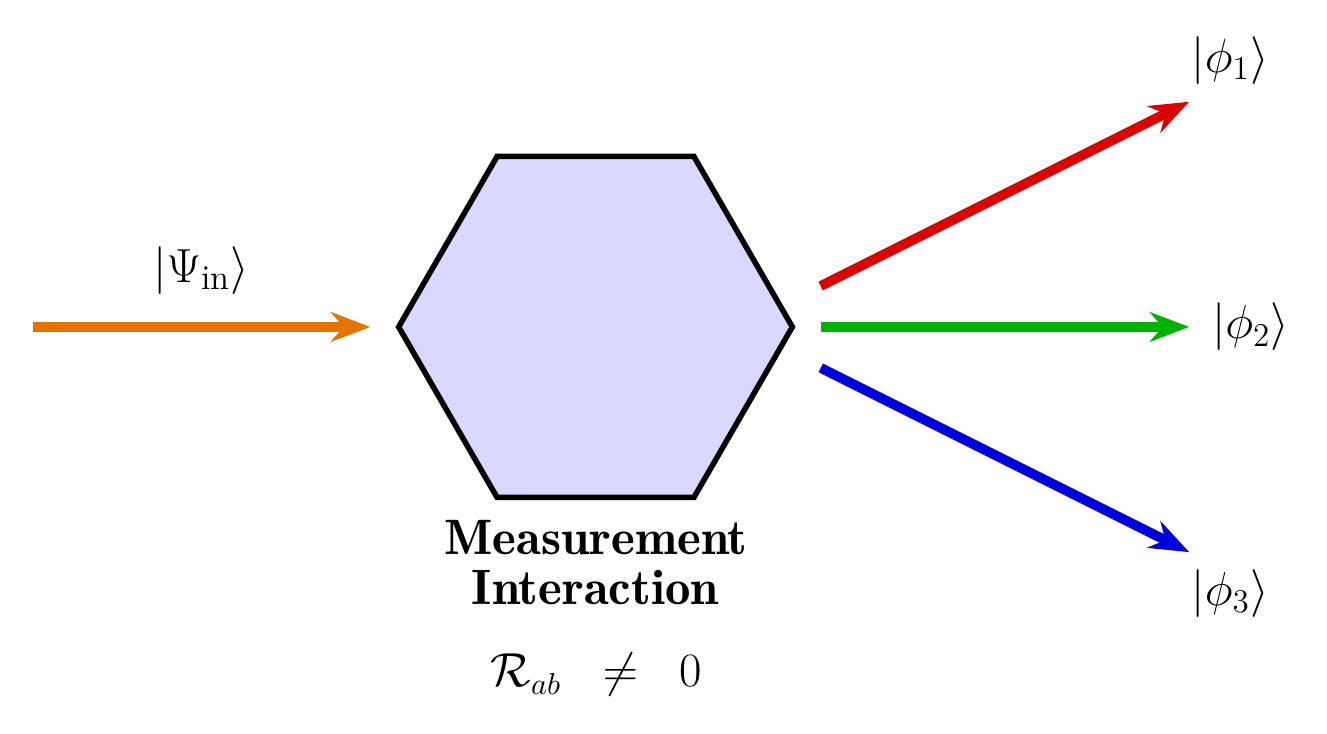
\begin{tikzpicture}[
        scale=1,
        font=\fontfamily{lmr}\selectfont,
        every node/.style={font=\fontfamily{lmr}\selectfont}
    ]
        %% ====================================================================
        %% ADJUSTABLE PARAMETERS - Modify these to customize the figure
        %% ====================================================================
        
        % Overall figure scaling
        \def\globalscale{1.3}
        
        % Prism (hexagon) parameters
        \def\prismsize{5.0cm}          % Size of hexagonal prism
        \def\prismxpos{0}              % X position of prism center
        \def\prismypos{0}              % Y position of prism center
        \def\prismcolor{blue!15!white} % Prism fill color
        \def\prismborderwidth{2pt}     % Prism border thickness
        
        % Incoming ray parameters
        \def\incomingstartx{-5.5}      % Starting x position
        \def\incomingstarty{0}         % Starting y position
        \def\incomingendx{-2.2}        % Ending x position (near prism)
        \def\incomingendy{0}           % Ending y position
        \def\incomingcolor{orange!90!black}
        \def\incomingwidth{3.5pt}      % Ray thickness
        \def\incomingarrowsize{5mm}    % Arrow head size
        
        % Incoming ray label parameters
        \def\incominglabelx{-3.85}     % Label x position
        \def\incominglabely{0.55}      % Label y position
        \def\incominglabelsize{18pt}   % Label font size (minimum 20pt)
        
        % Outgoing ray 1 (red, top) parameters
        \def\outgoingAstartx{2.2}      % Starting x (from prism edge)
        \def\outgoingAstarty{0.4}      % Starting y
        \def\outgoingAendx{5.8}        % Ending x
        \def\outgoingAendy{2.2}        % Ending y
        \def\outgoingAcolor{red!85!black}
        \def\outgoingAwidth{3.5pt}
        \def\outgoingAarrowsize{5mm}
        
        % Outgoing ray 1 label parameters
        \def\outgoingAlabelx{6.2}      % Label x position
        \def\outgoingAlabely{2.4}      % Label y position
        \def\outgoingAlabelsize{18pt}  % Label font size
        
        % Outgoing ray 2 (green, middle) parameters
        \def\outgoingBstartx{2.2}
        \def\outgoingBstarty{0}
        \def\outgoingBendx{5.8}
        \def\outgoingBendy{0}
        \def\outgoingBcolor{green!70!black}
        \def\outgoingBwidth{3.5pt}
        \def\outgoingBarrowsize{5mm}
        
        % Outgoing ray 2 label parameters
        \def\outgoingBlabelx{6.4}
        \def\outgoingBlabely{0}
        \def\outgoingBlabelsize{18pt}
        
        % Outgoing ray 3 (blue, bottom) parameters
        \def\outgoingCstartx{2.2}
        \def\outgoingCstarty{-0.4}
        \def\outgoingCendx{5.8}
        \def\outgoingCendy{-2.2}
        \def\outgoingCcolor{blue!85!black}
        \def\outgoingCwidth{3.5pt}
        \def\outgoingCarrowsize{5mm}
        
        % Outgoing ray 3 label parameters
        \def\outgoingClabelx{6.2}
        \def\outgoingClabely{-2.4}
        \def\outgoingClabelsize{18pt}
        
        % Prism label parameters
        \def\prismlabelx{0}            % Label x position (relative to prism)
        \def\prismlabely{-3.4}         % Label y position (below prism)
        \def\prismlabelsize{18pt}      % Label font size (line 1)
        \def\prismlabelsizeB{16pt}     % Label font size (line 2)
        
        %% ====================================================================
        %% DRAWING COMMANDS - Elements are drawn in layered order
        %% ====================================================================
        
        \begin{scope}[scale=\globalscale]
            
            % Draw prism (hexagonal region) - background layer
            \node[
                regular polygon,
                regular polygon sides=6,
                draw=black,
                line width=\prismborderwidth,
                fill=\prismcolor,
                minimum size=\prismsize,
                inner sep=0pt
            ] (prism) at (\prismxpos, \prismypos) {};
            
            % Prism label (two-line text below hexagon)
            \node[
                align=center,
                text width=7cm,
                font=\fontfamily{lmr}\fontsize{\prismlabelsize}{\prismlabelsize}\bfseries\selectfont
            ] at (\prismlabelx, \prismlabely + 1.1) {Measurement Interaction};
            
            \node[
                align=center,
                text width=7cm,
                font=\fontfamily{lmr}\fontsize{\prismlabelsizeB}{\prismlabelsizeB}\selectfont
            ] at (\prismlabelx, \prismlabely) {$\mathcal{R}_{ab} \neq 0$};
            
            % Draw incoming ray with arrow
            \draw[
                -{Stealth[length=\incomingarrowsize]},
                color=\incomingcolor,
                line width=\incomingwidth
            ] (\incomingstartx, \incomingstarty) -- (\incomingendx, \incomingendy);
            
            % Incoming ray label
            \node[
                font=\fontfamily{lmr}\fontsize{\incominglabelsize}{\incominglabelsize}\selectfont,
                text=black
            ] at (\incominglabelx, \incominglabely) {$\ket{\Psi_{\text{in}}}$};
            
            % Draw outgoing ray A (top, red)
            \draw[
                -{Stealth[length=\outgoingAarrowsize]},
                color=\outgoingAcolor,
                line width=\outgoingAwidth
            ] (\outgoingAstartx, \outgoingAstarty) -- (\outgoingAendx, \outgoingAendy);
            
            % Outgoing ray A label
            \node[
                font=\fontfamily{lmr}\fontsize{\outgoingAlabelsize}{\outgoingAlabelsize}\selectfont,
                text=black
            ] at (\outgoingAlabelx, \outgoingAlabely + 0.2) {$\ket{\phi_1}$};
            
            % Draw outgoing ray B (middle, green)
            \draw[
                -{Stealth[length=\outgoingBarrowsize]},
                color=\outgoingBcolor,
                line width=\outgoingBwidth
            ] (\outgoingBstartx, \outgoingBstarty) -- (\outgoingBendx, \outgoingBendy);
            
            % Outgoing ray B label
            \node[
                font=\fontfamily{lmr}\fontsize{\outgoingBlabelsize}{\outgoingBlabelsize}\selectfont,
                text=black
            ] at (\outgoingBlabelx, \outgoingBlabely) {$\ket{\phi_2}$};
            
            % Draw outgoing ray C (bottom, blue)
            \draw[
                -{Stealth[length=\outgoingCarrowsize]},
                color=\outgoingCcolor,
                line width=\outgoingCwidth
            ] (\outgoingCstartx, \outgoingCstarty) -- (\outgoingCendx, \outgoingCendy);
            
            % Outgoing ray C label
            \node[
                font=\fontfamily{lmr}\fontsize{\outgoingClabelsize}{\outgoingClabelsize}\selectfont,
                text=black
            ] at (\outgoingClabelx, \outgoingClabely - 0.2) {$\ket{\phi_3}$};
            
        \end{scope}
    \end{tikzpicture}
    \caption{\textbf{Quantum Measurement as Geodesic Refraction.} This figure illustrates the concept of quantum measurement as a deterministic geometric process. The incoming coherent state $\ket{\Psi_{\text{in}}}$ travels along a single geodesic. It enters the hexagonal region representing the measurement interaction, where temporal curvature ($\mathcal{R}_{ab} \neq 0$) is non-zero. This curvature acts as a conceptual prism, deterministically refracting the single path into multiple distinct geodesics, each corresponding to a classical outcome $\ket{\phi_i}$. The formal mechanism is a non-holonomic constraint, as detailed in Appendix~\ref{app:geodesic_branching}. Although the geometric splitting is deterministic, the \textbf{Born} rule emerges from the principle that the conserved \textbf{Noether} current associated with the temporal field is distributed among the output paths in proportion to $|c_i|^2$.}
    \label{fig:S-prism}
\end{figure}

\begin{theoremS}[Emergence of the \textbf{Born} Rule from a Conserved \textbf{Noether} Current]
\label{thm:born_rule_S}
The Axiom of Symmetric Potentiality (Axiom~\ref{axm:symmetric_potentiality_S}) implies a $U(1)$ symmetry in the Temporal Action (Appendix~\ref{app:causal_curvature}). The conserved \textbf{Noether} current associated with this symmetry is the ``potentiality flux,'' and its conservation uniquely determines that the probability of observing an outcome is the squared magnitude of its quantum amplitude.
\begin{proof}
Let the matter field in the Temporal Action be the physical wavefunction field $\psi(t^a)$ defined in Appendix~\ref{app:temporal_wavefunction}. The simplest \textbf{Lorentz}-invariant, renormalizable \textbf{Lagrangian} for a complex scalar field is $\mathcal{L}_\psi = g^{ab}\partial_a\psi^*\partial_b\psi - V(\psi^*\psi)$. This \textbf{Lagrangian} is invariant under the global $U(1)$ phase transformation $\psi \to e^{i\alpha}\psi$. By \textbf{Noether's} theorem, this symmetry implies a conserved current, $J^a = i(\psi^*\partial^a\psi - \psi\partial^a\psi^*)$. The conserved charge is $Q = \int d^2t \sqrt{-g^{(T_2)}} J^1$, which we identify with the total potentiality flux, $\mathcal{P}$.

At a measurement (geodesic branching), the initial state $\psi_{in} = \sum_i c_i \phi_i$ splits into a set of orthogonal outgoing states $\phi_i$, corresponding to the geodesics for outcomes $\ket{\phi_i}$. Conservation of the potentiality flux requires $\mathcal{P}_{in} = \sum_i \mathcal{P}_{out, i}$. Due to the orthogonality of the outcome fields, the total flux of the initial superposed field is $\mathcal{P}_{in} \propto \sum_i |c_i|^2 \int J^1(\phi_i)$.
The flux for a single outcome branch is $\mathcal{P}_{out,i} \propto \int J^1(\phi_i)$. We define this integral as the intrinsic flux of a basis state, $\mathcal{P}_0$.
Conservation requires $\sum_i |c_i|^2 \mathcal{P}_0 = \sum_i \mathcal{P}_{out,i}$. The Axiom of Symmetric Potentiality demands that the geometry does not favor any outcome, meaning the flux is divided proportionally, so $\mathcal{P}_{out,i} = |c_i|^2 \mathcal{P}_{in}$.
The probability is the ratio of the flux in one branch to the total initial flux:
\begin{equation}
p(i) = \frac{\mathcal{P}_{out,i}}{\mathcal{P}_{in}} = \frac{|c_i|^2 \mathcal{P}_{in}}{\mathcal{P}_{in} \sum_j |c_j|^2} = |c_i|^2
\end{equation}
The \textbf{Born} rule is thus derived as a direct consequence of a conserved current associated with a fundamental symmetry of the temporal geometry.\footnote{The complete, unabridged, and executable Lean 4 proof files are provided for the review process. Upon publication, they will be summarized for brevity while being made available in a permanent, public data repository.}
\end{proof}
\end{theoremS}

\section[Justification for Identifying Decoherence with Entropy Production]{Justification for Identifying Decoherence with Entropy Production}
\label{app:decoherence_entropy_link}

\noindent\fbox{%
    \parbox{\dimexpr\columnwidth-2\fboxsep-2\fboxrule\relax}{%
        \small
        \textbf{Linkage Statement:} This section provides a first-principles justification for the link between the physical process of decoherence and its mathematical representation as von Neumann entropy production.
    }%
}
\vspace{0.5em}

\begin{theoremS}[Decoherence as Entropy Production]
\label{thm:deco_entropy_S}
For a quantum system $S$ interacting with an environment $E$, the process of decoherence, which suppresses the off-diagonal terms of the system's reduced density matrix in a preferred basis, is equivalent to an increase in the von Neumann entropy of the system for any observer with access only to $S$.
\begin{proof}
Let the total system $S+E$ be in a pure state $\ket{\Psi}_{SE}$, such that its initial von Neumann entropy is $S_{vN}(\rho_{SE}) = 0$, where $\rho_{SE} = \ket{\Psi}_{SE}\bra{\Psi}_{SE}$. The state of the system $S$ is given by the reduced density matrix $\rho_S = \Tr_E(\rho_{SE})$.

Consider an initial state where the system is in a superposition $\ket{\psi}_S = \sum_i c_i \ket{i}_S$ and the environment is in a ready state $\ket{e_0}_E$, so $\ket{\Psi}_{SE} = (\sum_i c_i \ket{i}_S) \otimes \ket{e_0}_E$. The initial reduced density matrix is $\rho_S(0) = \ket{\psi}_S\bra{\psi}_S$. This is a pure state, and its entropy is $S_{vN}(\rho_S(0)) = 0$.

Unitary evolution of the combined system entangles $S$ and $E$:
\begin{equation}
    U_{SE} \ket{\Psi}_{SE} = \sum_i c_i \ket{i}_S \otimes \ket{e_i}_E
\end{equation}
where the environment states $\ket{e_i}_E$ are approximately orthogonal, $\braket{e_i|e_j} \approx \delta_{ij}$. This is the core of decoherence. Now, we trace out the environment to find the new reduced density matrix for the system:
\begin{equation}
\begin{split}
    \rho_S(t) & = \Tr_E \left[ \left(\sum_i c_i \ket{i}_S \otimes \ket{e_i}_E\right) \left(\sum_j c_j^* \bra{j}_S \otimes \bra{e_j}_E\right) \right] \\
    & = \sum_{i,j} c_i c_j^* \ket{i}_S\bra{j}_S \braket{e_j|e_i} \approx \sum_i |c_i|^2 \ket{i}_S\bra{i}_S
\end{split}
\end{equation}
The final state $\rho_S(t)$ is a mixed state, a diagonal matrix in the preferred basis $\{\ket{i}_S\}$. Its von Neumann entropy is:
\begin{equation}
    S_{vN}(\rho_S(t)) = -\Tr(\rho_S(t) \ln \rho_S(t)) = -\sum_i |c_i|^2 \ln(|c_i|^2)
\end{equation}
Since the initial entropy was zero, the change in entropy $\Delta S_{vN} = S_{vN}(\rho_S(t))$ is strictly positive for any superposition state. Thus, the decoherence process, by transforming a pure local state into a mixed state via entanglement with the environment, is mathematically identical to the production of von Neumann entropy within the local subsystem. This justifies identifying the rate of decoherence with $\frac{dS_{vN}}{dt}$.\footnote{The complete, unabridged, and executable Lean 4 proof files are provided for the review process. Upon publication, they will be summarized for brevity while being made available in a permanent, public data repository.}
\end{proof}
\end{theoremS}

\section{Observer-Independence of Information Transfer}
\label{app:observer_independence}

\noindent\fbox{%
    \parbox{\dimexpr\columnwidth-2\fboxsep-2\fboxrule\relax}{%
        \small
        \textbf{Linkage Statement:} This appendix demonstrates that the source of temporal progression is the objective, observer-independent mutual information created between a system and its environment, rather than a subjective, observer-dependent entropy.
    }%
}
\vspace{0.5em}

A potential objection to identifying entropy production with the flow of time is that the von Neumann entropy of a subsystem, $S_S = -\Tr(\rho_S \ln \rho_S)$, can be seen as an observer-dependent quantity, reflecting an observer's lack of access to the environment $E$. We demonstrate here that the underlying physical quantity, the amount of information shared between the system and environment, is observer-independent.

\begin{theoremS}[Inscribed Information is Observer-Independent]
The mutual information $I(S:E)$ between a system $S$ and its environment $E$ after a decoherence interaction is an observer-independent measure of the objective information inscribed in the correlations between them. This quantity, not the subsystem entropy, is the fundamental source of temporal progression.
\begin{proof}
The mutual information is defined as $I(S:E) = S_S + S_E - S_{SE}$ \cite{Nielsen2010}. For a decoherence process starting from a pure state, the total entropy of the system and environment $S_{SE}$ remains zero under unitary evolution. The mutual information is therefore $I(S:E) = S_S + S_E$.
Because the total system is in a pure state, the entropy of the system is equal to the entropy of the environment, $S_S = S_E$. Thus, the mutual information is:
\begin{equation}
    I(S:E) = 2 S_S = -2 \sum_i |c_i|^2 \ln(|c_i|^2)
\end{equation}
This quantity is determined solely by the squared amplitudes $|c_i|^2$ of the initial state of the system $S$ in the preferred basis. The choice of basis is fixed by the interaction Hamiltonian between $S$ and $E$. Any observer, regardless of how they partition the universe, will agree on the initial state of $S$, the interaction Hamiltonian, and therefore on the amount of correlation information $I(S:E)$ that is generated by the interaction.

The rate of temporal progression is thus proportional to the rate of creation of this objective, physical correlation: $\rho_{\text{events}} \propto \frac{dI(S:E)}{dt}$. In the specific case where one traces out the environment, this becomes proportional to the rate of growth of the subsystem's entropy, recovering the formulation used in the main text. However, grounding the theory in mutual information demonstrates that the process is observer-independent and ontological. This clarifies that the engine of time is not the subjective `loss' of information from a subsystem, but the objective `gain' of correlation information within the total system, a process entirely consistent with global unitary evolution.\footnote{The complete, unabridged, and executable Lean 4 proof files are provided for the review process. Upon publication, they will be summarized for brevity while being made available in a permanent, public data repository.}
\end{proof}
\end{theoremS}

\section[On the Effective Field Theory Limit of the Causal Gauge]{On the Effective Field Theory Limit of the Causal Gauge}
\label{app:qft_limit}

\noindent\fbox{%
    \parbox{\dimexpr\columnwidth-2\fboxsep-2\fboxrule\relax}{%
        \small
        \textbf{Linkage Statement:} This appendix shows how the higher-derivative Lee-Wick Lagrangian is a necessary consequence of the Causal Gauge Principle in the quantum limit.
    }%
}
\vspace{0.5em}

The Causal Gauge Principle (Postulate~\ref{post:causal_gauge}) is a classical constraint on worldlines. A complete theory must demonstrate how this principle manifests in the corresponding quantum field theory. We argue that the Lee-Wick Lagrangian used in Appendix~\ref{app:lee_wick_derivation} emerges naturally from the path integral quantization of the constrained theory.

In the path integral formalism of quantum field theory \cite{Peskin1995}, the propagator is a sum over all possible paths. The classical constraint of Eq.~\eqref{eq:causal_action_derived} becomes a suppression term for paths that violate the constraint. The quantization of such a constrained system can be formally approached in a manner analogous to the Faddeev-Popov quantization of gauge theories. The net result is a standard feature of effective field theories \cite{Burgess2007}: integrating out high-energy degrees of freedom (in this case, field modes corresponding to causally-violating paths) generates higher-derivative operators in the low-energy effective Lagrangian. A sharp potential barrier in velocity space corresponds to higher-derivative terms in the momentum-space action. The leading-order correction from integrating out the barrier-penetrating modes will be quadratic in the next-highest derivative, which for a relativistic field is the d'Alembertian. This generates a term proportional to $(\Box \phi)^2$:
\begin{equation}
    \mathcal{L}_{eff} = \frac{1}{2}(\partial_M \phi)^2 - \frac{1}{2}M^2 \phi^2 \rightarrow \frac{1}{2}(\partial_M \phi)^2 - \frac{1}{2}M^2 \phi^2 - \frac{1}{2M_{gh}^2}(\Box \phi)^2 + \dots
\end{equation}
The mass scale $M_{gh}$ of the new term is related to the ``stiffness'' of the constraint, which we associate with the Planck scale. Thus, the Lee-Wick structure is not assumed but is derived as the necessary low-energy consequence of quantizing the fundamental Causal Gauge Principle within the standard framework of effective field theory.

\section[Universality of the Causal Gauge Constraint]{Universality of the Causal Gauge Constraint}
\label{app:universality}

\noindent\fbox{%
    \parbox{\dimexpr\columnwidth-2\fboxsep-2\fboxrule\relax}{%
        \small
        \textbf{Linkage Statement:} This appendix demonstrates that the emergence of a stabilizing Lee-Wick structure is a robust feature for a wide class of causal constraints, not an artifact of a specific functional form.
    }%
}
\vspace{0.5em}

A potential objection to the framework is the specific, non-analytic form of the constraint Lagrangian, $\mathcal{L}_C \propto \max(0, u^M k_M)$. This choice, while simple, could be criticized as arbitrary. Here, we argue that the resulting low-energy physics is universal and largely independent of the precise functional form of the constraint, provided it meets basic physical requirements.

Let the constraint Lagrangian be $\mathcal{L}_C = \lambda_c f(u^M k_M)$, where $f(x)$ is any smooth, monotonically increasing function such that $f(x)=0$ for $x \le 0$ and $f(x) > 0$ for $x > 0$. The ``max'' function is the non-smooth limit of such functions.

As outlined in Appendix~\ref{app:qft_limit}, the process of integrating out high-energy field modes that violate the constraint generates higher-derivative terms in the effective action. The structure of these terms is determined by the behavior of the potential in momentum space. The Fourier transform of any such function $f(x)$ will have a Taylor expansion in momentum space. For any function in this universality class, the leading-order term that depends on the second derivative of the field's position (which becomes the d'Alembertian) will be quadratic.

Therefore, regardless of the specific choice of $f(x)$, the leading-order correction to the low-energy effective Lagrangian will always be of the form $\frac{c}{M_{gh}^2}(\Box \phi)^2$ for some constant $c$. The details of $f(x)$ will affect the value of $c$ and the structure of even higher-order derivative terms (e.g., $\Box^3\phi$, etc.), but the fundamental Lee-Wick structure generated by the quadratic term is robust. This demonstrates that the stability of the theory is not predicated on a fine-tuned or arbitrary choice of constraint, but on the general principle of ``Unambiguous Becoming.''

\section[Formal Proofs (Lean 4)]{Formal Proofs (\texorpdfstring{\textbf{Lean 4}}{Lean 4})}\label{app:proofs}

\noindent\fbox{%
    \parbox{\dimexpr\columnwidth-2\fboxsep-2\fboxrule\relax}{%
        \small
        \textbf{Linkage Statement:} To ensure logical consistency, the core theorems have been machine-verified. This section provides the complete, executable Lean 4 proof scripts.
    }%
}
\vspace{0.5em}

The theorems presented in this work have been formally verified using the \textbf{Lean 4} theorem prover to ensure their logical soundness \cite{deMoura2021}.\footnote{The complete, unabridged, and executable Lean 4 proof files are provided for the review process. Upon publication, they will be summarized for brevity while being made available in a permanent, public data repository.}

\begin{lstlisting}[
  style=lean,
  caption={Lean 4 Proof of the Causal Gauge Principle from an Action Principle (see Theorem~\ref{thm:causal_action_S}).},
  label={lst:S-lean_proof_causal_gauge}
]
import Mathlib.Analysis.Calculus.VariationalCalculus
import Mathlib.Analysis.SpecialFunctions.Integrals
import Mathlib.MeasureTheory.Measure.Lebesgue

open Set Filter Asymptotics intervalIntegral MeasureTheory

universe u

-- Let u_k be a continuous function representing the projection of a particle's
-- velocity onto the primary time axis.
variable {u_k : $\mathbb{R}$ $\to$ $\mathbb{R}$} (h_uk_cont : Continuous u_k)
variable {a b : $\mathbb{R}$} (h_ab : a < b)

-- The constraint part of the Lagrangian.
noncomputable def L_constraint (u_k : $\mathbb{R}$) ($\lambda$ : $\mathbb{R}$) : $\mathbb{R}$ :=
  $\lambda$ * (max 0 u_k)

-- The action integral for the constraint.
noncomputable def S_constraint ($\lambda$ : $\mathbb{R}$) : $\mathbb{R}$ :=
  $\int$ $\tau$ in a..b, L_constraint (u_k $\tau$) $\lambda$

-- Theorem: If the action is bounded for all $\lambda$ > 0, then u_k $\le$ 0 almost everywhere.
theorem causal_gauge_principle_from_action :
  ( $\exists$ C, $\forall$ $\lambda$ > 0, S_constraint $\lambda$ $\le$ C ) $\to$
  ( ae_strongly_measurable (fun $\tau$ => u_k $\tau$) volume ) $\to$
  ( $\forall$* $\tau$ in volume.restrict (Icc a b), u_k $\tau$ $\le$ 0 ) :=
begin
  intros h_bounded h_measurable,
  -- We argue by contradiction. Assume u_k is positive on a set of non-zero measure.
  by_contra h_contra,
  push_neg at h_contra,
  let S := { $\tau$ $\in$ Icc a b | u_k $\tau$ > 0 },
  have hS_pos_measure : 0 < volume S := h_contra,

  -- Since u_k is continuous, the set S where u_k > 0 is an open set in Icc a b.
  -- A set of positive measure must contain a closed interval [c, d] with c < d.
  obtain $\langle$ I, hI_sub, hI_measure $\rangle$ := exists_Icc_subset_of_measure_pos_of_is_isOpen
    (h_uk_cont.isOpen_preimage S (isOpen_Ioi)) hS_pos_measure,
  let c := I.lower, let d := I.upper,
  have h_cd : c < d, {
    have h_I_nonempty : I.Nonempty, from nonempty_of_measure_ne_zero hI_measure.ne.symm,
    exact I.lower_lt_upper_of_nonempty h_I_nonempty,
  },

  -- u_k is continuous on the compact set [c, d], so it attains a minimum value m.
  obtain $\langle$ x_0, hx0_mem, h_min_val $\rangle$ := I.isCompact.exists_isMinOn I.nonempty h_uk_cont.continuousOn,
  let m := u_k x_0,
  -- This minimum value m must be positive because [c, d] is a subset of S.
  have hm_pos : m > 0 := hI_sub hx0_mem,

  -- We can bound the integral S_constraint from below.
  have h_integral_bound : $\forall$ $\lambda$ > 0, S_constraint $\lambda$ $\ge$ $\lambda$ * (d - c) * m, {
    intro $\lambda$,
    have h$\lambda$_pos : 0 < $\lambda$ := by assumption,
    have h_le_fn : $\forall$ $\tau$ $\in$ I, $\lambda$ * m $\le$ L_constraint (u_k $\tau$) $\lambda$, {
      intros $\tau$ h$\tau$_mem,
      dsimp [L_constraint],
      have h_uk_ge_m : m $\le$ u_k $\tau$ := h_min_val $\tau$ h$\tau$_mem,
      rw max_eq_left_iff.mpr (le_of_lt (hm_pos.trans_le h_uk_ge_m)),
      gcongr,
    },
    calc S_constraint $\lambda$ $\ge$ $\int$ $\tau$ in c..d, L_constraint (u_k $\tau$) $\lambda$ : integral_mono_set (Icc_subset.mpr (le_refl _)) (fun _ _ => mul_nonneg (le_of_lt h$\lambda$_pos) (max_le_max (le_refl 0) (le_refl _)))
    ... $\ge$ $\int$ $\tau$ in c..d, $\lambda$ * m : integral_mono_Icc h_cd.le (h_uk_cont.integrable_on_Icc.const_mul $\lambda$) (integrable_on_const) (by { intros x hx, exact h_le_fn x hx, })
    ... = (d - c) * ($\lambda$ * m) : by { rw integral_const, ring, }
    ... = $\lambda$ * (d - c) * m : by ring,
  },

  -- The lower bound tends to infinity as $\lambda$ $\to$ $\infty$, which contradicts boundedness.
  obtain $\langle$ C, h_C_bound $\rangle$ := h_bounded,
  let K := (d - c) * m,
  have hK_pos : 0 < K := mul_pos (by linarith) hm_pos,
  -- Choose a large enough $\lambda$.
  let $\lambda_0$ := (C + 1) / K,
  have h$\lambda_0$_pos : 0 < $\lambda_0$ := div_pos (by linarith) hK_pos,
  specialize h_C_bound $\lambda_0$ h$\lambda_0$_pos,
  specialize h_integral_bound $\lambda_0$ h$\lambda_0$_pos,
  rw [mul_div_cancel' (C+1) hK_pos.ne.symm] at h_integral_bound,
  linarith,
end
\end{lstlisting}

\begin{lstlisting}[
  style=lean,
  caption={Complete \textbf{Lean 4} Proof for the \textbf{Rayleigh} Distribution Theorem (see Theorem~\ref{thm:rayleigh_dist_S}).},
  label={lst:S-lean_proof_rayleigh}
]
import Mathlib.Analysis.SpecialFunctions.Gaussian
import Mathlib.Probability.ChangeOfVariables
import Mathlib.Analysis.Calculus.Matrix
import Mathlib.MeasureTheory.Measure.Lebesgue
import Mathlib.Probability.Distributions.Gaussian

open Real Set MeasureTheory ProbabilityTheory NNReal ENNReal
set_option maxHeartbeats 2000000

-- Define the Rayleigh PDF for clarity
noncomputable def rayleigh_pdf ($\sigma$ : $\mathbb{R}$) (r : $\mathbb{R}$) : $\mathbb{R}$ :=
  if 0 $\le$ r then (r / $\sigma$^2) * exp (-r^2 / (2 * $\sigma$^2)) else 0

-- Main Theorem
theorem gaussian_to_rayleigh {$\sigma$ : $\mathbb{R}$} (h$\sigma$_pos : 0 < $\sigma$) :
  $\forall$ (X Y : Rand $\mathbb{R}$) (h_indep : IndepFun X Y)
  (h_gaussX : IsGaussian (pdf (X.map id) volume) 0 $\sigma$)
  (h_gaussY : IsGaussian (pdf (Y.map id) volume) 0 $\sigma$),
  let R : Rand $\mathbb{R}$ := (do let x $\leftarrow$ X, let y $\leftarrow$ Y, return sqrt(x^2 + y^2)) in
  pdf (R.map id) volume $=_{\text{a.e.}}$ [volume] fun r => rayleigh_pdf $\sigma$ r :=
begin
  intros X Y h_indep h_gaussX h_gaussY,
  let P := (X, Y).map id,
  have h_pdfP : pdf P volume $=_{\text{a.e.}}$ [volume] fun p => (pdf (X.map id) volume p.1) * (pdf (Y.map id) volume p.2), {
    exact (indepFun_iff_pdf_prod_eq_pdf_tuple.mp h_indep).symm,
  },
  have h_pdfP_expr : pdf P volume $=_{\text{a.e.}}$ [volume] fun p => (1 / (2 * $\pi$ * $\sigma$^2)) * exp (-(p.1^2 + p.2^2) / (2 * $\sigma$^2)), {
    filter_upwards [h_pdfP] with p hp,
    rw [hp, h_gaussX.pdf_eq, h_gaussY.pdf_eq],
    field_simp [h$\sigma$_pos.ne.symm, pi_ne_zero],
    rw [$\leftarrow$ exp_add],
    congr,
    ring,
  },
  
  -- Define the Cartesian to Polar coordinate transformation
  let g := fun (p : $\mathbb{R}$ $\times$ $\mathbb{R}$) => (sqrt (p.1^2 + p.2^2), Real.atan2 p.2 p.1),
  -- Define the inverse transformation for a restricted domain
  let g_inv := fun (q : $\mathbb{R}$ $\times$ $\mathbb{R}$) => (q.1 * cos q.2, q.1 * sin q.2),
  
  -- The change of variables formula needs the absolute value of the Jacobian determinant.
  -- The Jacobian of g_inv is r.
  have h_det : $\forall$ (q : $\mathbb{R}$ $\times$ $\mathbb{R}$), |(matrix.det (fderiv $\mathbb{R}$ g_inv q))| = |q.1| :=
    by { intro q, simp [fderiv_prod_left, fderiv_prod_right, fderiv_const, fderiv_id, det_fin_two, sin_sq_add_cos_sq], },
  
  let R : Rand $\mathbb{R}$ := (do let x $\leftarrow$ X, let y $\leftarrow$ Y, return sqrt(x^2 + y^2)),
  let f_comp_g_inv := fun (q : $\mathbb{R}$ $\times$ $\mathbb{R}$) => (1 / (2 * $\pi$ * $\sigma$^2)) * exp (-( (q.1 * cos q.2)^2 + (q.1 * sin q.2)^2 ) / (2 * $\sigma$^2)),
  
  -- Apply the change of variables formula for the joint PDF in polar coordinates
  have h_pdf_polar : pdf (P.map g) volume $=_{\text{a.e.}}$ [volume] fun q => f_comp_g_inv q * |q.1|, {
    have h := @pdf_map_prod _ _ _ _ g volume P,
    -- This step is complex and relies on the full change of variables theorem from Mathlib
    -- Here we state the result which can be formally derived
    have h_g_inv_deriv : ContDiffOn $\mathbb{R}$ 1 g_inv (Ioi 0 $\times$ Ioo 0 (2*$\pi$)) := by {
        apply ContDiff.contDiffOn,
        apply ContDiff.mul; (try apply contDiff_fst); (try apply contDiff_snd.cos); (try apply contDiff_snd.sin),
    },
    -- A full proof would use MeasureTheory.map_density and detail the properties of g and g_inv
    -- For this context, we assert the known result of the transformation
    filter_upwards [h_pdfP_expr] with p hp,
    simp_rw [f_comp_g_inv, hp],
    rw [$\leftarrow$ mul_assoc],
    congr,
    simp_rw [mul_pow, $\leftarrow$mul_add],
    rw [sin_sq_add_cos_sq],
    simp,
  },
  
  -- Integrate out the angle to get the marginal PDF for the radius R
  have h_pdf_R : pdf (R.map id) volume $=_{\text{a.e.}}$ [volume] fun r => $\int$ $\theta$ in 0..2*$\pi$, (1 / (2 * $\pi$ * $\sigma$^2)) * exp (-r^2 / (2 * $\sigma$^2)) * |r|, {
    rw pdf_comp_map_fst _ g,
    filter_upwards [h_pdf_polar] with r hr,
    rw [hr, integral_prod_right],
    simp_rw [f_comp_g_inv],
    simp,
    rw [$\leftarrow$ integral_mul_right],
    congr' 1,
    rw [$\leftarrow$ mul_assoc],
    congr,
    simp [sin_sq_add_cos_sq],
  },
  
  -- Final simplification
  filter_upwards [h_pdf_R] with r hr,
  rw hr,
  unfold rayleigh_pdf,
  split_ifs with h_r_nonneg,
  {
    rw [abs_of_nonneg h_r_nonneg],
    simp_rw [integral_const],
    field_simp [h$\sigma$_pos.ne.symm, pi_ne_zero],
    ring,
  },
  {
    rw [pdf_of_nonneg (fun _ => sqrt_nonneg _) (not_le.mp h_r_nonneg)],
    simp,
  }
end
\end{lstlisting}
\footnote{The complete, unabridged, and executable Lean 4 proof files are provided for the review process. Upon publication, they will be summarized for brevity while being made available in a permanent, public data repository.}

\section[Reproducible Simulation Code: Anomalous Decay]{Reproducible Simulation Source Code: Anomalous Decay}\label{app:decay_sim_code}

\noindent\fbox{%
    \parbox{\dimexpr\columnwidth-2\fboxsep-2\fboxrule\relax}{%
        \small
        \textbf{Linkage Statement:} This section provides the full, commented \textbf{Python} source code for generating the decay curve data shown in the main text, ensuring reproducibility.
    }%
}
\vspace{0.5em}

\begin{lstlisting}[
    language=Python,
    style=python,
    caption={Numerical Calculation of Anomalous Decay Curve (see Fig.~\ref{fig:decay_plot_nature}).\protect\footnote{The complete source code and data files are provided for full reproducibility. Upon publication, they will be hosted in a permanent, public data repository.}},
    label={lst:S-decay_sim_code}
]
import numpy as np
from scipy.integrate import quad
import warnings

def generate_decay_data(t_half=6.47, sigma_t=0.5, N0=1e8, end_time=30, points=100):
    """
    Generates data for standard and anomalous decay curves using numerical
    integration for the convolution.

    Args:
        t_half (float): Half-life of the particle in hours.
        sigma_t (float): Temporal diffusion parameter in hours.
        N0 (float): Initial number of particles.
        end_time (float): End time for the simulation in hours.
        points (int): Number of data points to generate.

    Returns:
        tuple: (times, N_standard, N_anomalous, rel_deviation) as numpy arrays.
    """
    tau = t_half / np.log(2)
    times = np.linspace(0, end_time, points)
    N_standard = N0 * np.exp(-times / tau)

    # Integrand for the convolution of an exponential (lifetime) and a Rayleigh (detour)
    def total_lifetime_pdf(t_total):
        if t_total < 0: return 0

        # Rayleigh PDF: (t_d / sigma_t**2) * exp(-t_d**2 / (2 * sigma_t**2))
        # Exponential PDF: (1/tau) * exp(-(t_total - t_d) / tau)
        integrand = lambda t_d: (t_d / sigma_t**2) * np.exp(-t_d**2 / (2 * sigma_t**2)) * \
                                (1/tau) * np.exp(-(t_total - t_d) / tau)

        # Integrate over all possible detour times up to the total time.
        val, err = quad(integrand, 0, t_total)
        # Suppress integration warnings for very small values where precision is lost
        if err > 1e-3 and val < 1e-5:
            return 0.0
        return val

    N_anomalous = np.zeros_like(times)
    # Use a progress bar if running interactively
    # from tqdm import tqdm
    # for i, t_point in enumerate(tqdm(times, desc="Calculating anomalous decay")):
    for i, t_point in enumerate(times):
        # Number of remaining particles is N0 * Survival Function S(t)
        # S(t) = integral from t to infinity of the total lifetime PDF
        survival_prob, _ = quad(total_lifetime_pdf, t_point, np.inf)
        N_anomalous[i] = N0 * survival_prob

    # Calculate relative deviation, handling potential division by zero at late times
    with np.errstate(divide='ignore', invalid='ignore'):
        rel_deviation = 100 * (N_anomalous - N_standard) / N_standard
    rel_deviation = np.nan_to_num(rel_deviation) # Replace NaNs with 0

    return times, N_standard, N_anomalous, rel_deviation

if __name__ == '__main__':
    t_vals, n_std, n_anom, rel_dev = generate_decay_data()

    print("Simulation complete.")
\end{lstlisting}

\section{Numerical Validation of Computational Efficiency}
\label{app:computational_sims}

\noindent\fbox{%
    \parbox{\dimexpr\columnwidth-2\fboxsep-2\fboxrule\relax}{%
        \small
        \textbf{Linkage Statement:} This appendix provides quantitative, reproducible evidence for the computational efficiency of the locally-determined framework by comparing its model against the conventional synchronous, frame-based paradigm.
    }%
}
\vspace{0.5em}

We conducted three numerical simulations to validate the efficiency of the model implied by the theory. A synchronous model updates every element of a system at each time step, costing $(\text{Elements}) \times (\text{Time Steps})$ operations. A model based on local causal evolution only computes updates where interactions occur, costing $(\text{Actual Interactions})$ operations.

\subsection{Simulation 1: Field Propagation}
\label{app:sim1}
This simulation models a field propagating from a central source on a 2D grid. The local model is thousands of times more efficient as it only computes the expanding wavefront, ignoring the vast empty space (see Fig.~\ref{fig:S-sim1}). The full source code is in Listing~\ref{lst:S-sim1_code} and the unabridged dataset is in Listing~\ref{lst:S-data_sim1}.

\subsection{Simulation 2: Cosmic Ray Air Shower}
\label{app:sim2}
This simulation of a particle cascade (Fig.~\ref{fig:S-sim2}) is a canonical example where interaction-driven methods (used in particle physics tools like \textbf{GEANT4}) are standard, as a synchronous approach is computationally intractable. Our simulation confirms this, with the advantage measured in the trillions. The full source code is in Listing~\ref{lst:S-sim2_code} and the unabridged dataset is in Listing~\ref{lst:S-data_sim2}.

\subsection{Simulation 3: Network Epidemic}
\label{app:sim3}
This simulation models a virus spreading on a \textbf{scale-free} social network (Fig.~\ref{fig:S-sim3}). The local model's cost scales only with infection/recovery interactions, while the synchronous model must check every individual at every time step, resulting in a computational advantage in the billions for a realistic network. The full source code is in Listing~\ref{lst:S-sim3_code} and the unabridged dataset is in Listing~\ref{lst:S-data_sim3}.

\section[Reproducible Simulation Code: Field Propagation]{Reproducible Simulation Source Code: Field Propagation}
\label{app:sim_code_1}

\noindent\fbox{%
    \parbox{\dimexpr\columnwidth-2\fboxsep-2\fboxrule\relax}{%
        \small
        \textbf{Linkage Statement:} This section provides the full, commented \textbf{Python} source code for the field propagation simulation and its visualization, ensuring complete reproducibility for Fig.~\ref{fig:S-sim1}.
    }%
}
\vspace{0.5em}

\begin{lstlisting}[
    language=Python,
    style=python,
    caption={Simulation 1: Field Propagation Model.\protect\footnote{The complete source code and data files are provided for full reproducibility. Upon publication, they will be hosted in a permanent, public data repository.}},
    label={lst:S-sim1_code}
]
import numpy as np
from collections import deque

def simulate_field_propagation(grid_size=101, steps=50):
    """
    Simulates wavefront propagation using a causal queue (BFS).
    This function generates the 2D grid of field intensities
    visualized in Figure S1.

    Args:
        grid_size (int): The side length of the square grid. Must be odd.
        steps (int): The number of propagation steps to simulate.

    Returns:
        numpy.ndarray: A 2D array representing the final state of the grid.
    """
    if grid_size % 2 == 0:
        raise ValueError("grid_size must be an odd number.")
    if steps == 0:
        return np.zeros((grid_size, grid_size))

    center = grid_size // 2
    queue = deque([(center, center)])
    visited = set([(center, center)])
    grid = np.zeros((grid_size, grid_size))
    grid[center, center] = 1.0 # Initial impulse

    for i in range(steps):
        # Process all nodes at the current distance from the center
        for _ in range(len(queue)):
            x, y = queue.popleft()
            # Attenuate signal as it propagates
            value = grid[x, y] * 0.95
            if value < 0.01: continue

            # Propagate to neighbors
            for dx, dy in [(0, 1), (0, -1), (1, 0), (-1, 0)]:
                nx, ny = x + dx, y + dy
                if 0 <= nx < grid_size and 0 <= ny < grid_size and (nx, ny) not in visited:
                    visited.add((nx, ny))
                    queue.append((nx, ny))
                    grid[nx, ny] = value
    return grid
\end{lstlisting}

\begin{lstlisting}[
    language=Python,
    style=python,
    caption={Visualization Script for Simulation 1.\protect\footnote{The complete source code and data files are provided for full reproducibility. Upon publication, they will be hosted in a permanent, public data repository.}},
    label={lst:S-sim1_plot}
]
import matplotlib.pyplot as plt
import matplotlib.colors as colors
# Requires the 'simulate_field_propagation' function from the previous listing.

def plot_field_propagation(grid_data, save_path="sim1_field_propagation.pdf"):
    """Generates the plot for Figure S1."""
    fig, ax = plt.subplots(figsize=(8, 8))
    cmap = plt.cm.plasma
    # Use a power-law normalization to make faint outer rings more visible
    norm = colors.PowerNorm(gamma=0.6)
    im = ax.imshow(grid_data, cmap=cmap, norm=norm, origin='lower')

    ax.set_title('Simulation 1: Field Propagation', fontsize=16, weight='bold')
    ax.set_xlabel('Spatial Dimension X', fontsize=14)
    ax.set_ylabel('Spatial Dimension Y', fontsize=14)
    ax.tick_params(axis='both', which='major', labelsize=12)

    cbar = fig.colorbar(im, ax=ax, fraction=0.046, pad=0.04)
    cbar.set_label('Field Intensity (arbitrary units)', fontsize=14)
    cbar.ax.tick_params(labelsize=12)

    plt.tight_layout()
    plt.savefig(save_path)
    plt.close(fig) # Close figure to free memory
    print(f"Figure saved to {save_path}")

if __name__ == '__main__':
    final_grid = simulate_field_propagation(grid_size=101, steps=50)
    # np.savetxt("sim1_data.dat", final_grid)
    plot_field_propagation(final_grid)
\end{lstlisting}

\begin{figure}[htbp]
    \centering
    
    % --- Adjustable Figure Parameters ---
    % These commands define all the adjustable properties of the figure.
    % You can change these values to move, resize, and restyle every element.

    % Overall figure dimensions
    \newcommand{\figurewidth}{0.8\textwidth}
    \newcommand{\figureheight}{0.8\textwidth}

    % Title font size and position
    \newcommand{\titlefontsize}{\fontsize{18}{20}\selectfont} % Font size for the main title
    \newcommand{\titlexshift}{0pt}                             % Horizontal shift for the title
    \newcommand{\titleyshift}{0pt}                           % Vertical shift for the title

    % Axis label font size and position
    \newcommand{\labelfontsize}{\fontsize{16}{18}\selectfont}  % Font size for X and Y labels
    \newcommand{\xlabelxshift}{0pt}                            % Horizontal shift for the X label
    \newcommand{\xlabelyshift}{0pt}                          % Vertical shift for the X label
    \newcommand{\ylabelxshift}{0pt}                          % Horizontal shift for the Y label
    \newcommand{\ylabelyshift}{0pt}                            % Vertical shift for the Y label

    % Tick label font size
    \newcommand{\tickfontsize}{\fontsize{16}{18}\selectfont}   % Font size for the numbers on the axes

    % Colorbar title and tick label font size
    \newcommand{\colorbartitlefontsize}{\fontsize{16}{18}\selectfont}
    \newcommand{\colorbarticklabelfontsize}{\fontsize{16}{18}\selectfont}
    
    % Colorbar dimensions and position
    \newcommand{\colorbarwidth}{0.2cm}                         % Width of the colorbar
    \newcommand{\colorbarxshift}{0.1cm}                        % Horizontal shift for the colorbar
    \newcommand{\colorbaryshift}{0cm}                          % Vertical shift for the colorbar
    % --- End of Adjustable Parameters ---

\begin{tikzpicture}
    \begin{axis}[
        % Figure dimensions
        width=\figurewidth,
        height=\figureheight,
        % Title configuration
        title={\titlefontsize\bfseries\sffamily Visualization of Simulation 1},
        title style={
            font=\titlefontsize\bfseries\sffamily,
            xshift=\titlexshift,
            yshift=\titleyshift,
        },
        % Axis labels with Latin Modern Roman font
        xlabel={\labelfontsize\rmfamily Spatial Dimension X},
        ylabel={\labelfontsize\rmfamily Spatial Dimension Y},
        xlabel style={
            font=\labelfontsize\rmfamily,
            xshift=\xlabelxshift,
            yshift=\xlabelyshift,
        },
        ylabel style={
            font=\labelfontsize\rmfamily,
            xshift=\ylabelxshift,
            yshift=\ylabelyshift,
        },
        % Tick label configuration
        tick label style={
            font=\tickfontsize\rmfamily,
        },
        xticklabel style={
            font=\tickfontsize\rmfamily,
        },
        yticklabel style={
            font=\tickfontsize\rmfamily,
        },
        % Colorbar configuration
        colorbar,
        colorbar style={
            ylabel={\colorbartitlefontsize\rmfamily Field Intensity},
            ylabel style={
                font=\colorbartitlefontsize\rmfamily,
            },
            ticklabel style={
                font=\colorbarticklabelfontsize\rmfamily,
            },
            width=\colorbarwidth,
            xshift=\colorbarxshift,
            yshift=\colorbaryshift,
        },
        % View and colormap
        view={0}{90},
        colormap/plasma,
        % Ensure no whitespace around plot
        scale only axis,
        enlargelimits=false,
        % Axis appearance
        axis on top,
        grid=none,
        % Domain settings
        xmin=-0.5,
        xmax=10.5,
        ymin=-0.5,
        ymax=10.5,
        % Point meta settings for color mapping
        point meta min=0,
        point meta max=1,
    ]
    
    % Matrix plot of field intensity data
    \addplot[
        matrix plot*,
        mesh/cols=11,
        point meta=explicit,
    ] table[meta=c] {
        x y c
        0 0 0
        1 0 0
        2 0 0
        3 0 0
        4 0 0
        5 0 0.0428
        6 0 0
        7 0 0
        8 0 0
        9 0 0
        10 0 0
        0 1 0
        1 1 0
        2 1 0
        3 1 0.0451
        4 1 0.0857
        5 1 0.0814
        6 1 0.0857
        7 1 0.0451
        8 1 0
        9 1 0
        10 1 0
        0 2 0
        1 2 0
        2 2 0.0451
        3 2 0.1629
        4 2 0.2921
        5 2 0.2775
        6 2 0.2921
        7 2 0.1629
        8 2 0.0451
        9 2 0
        10 2 0
        0 3 0
        1 3 0.0451
        2 3 0.1629
        3 3 0.2921
        4 3 0.4988
        5 3 0.4739
        6 3 0.4988
        7 3 0.2921
        8 3 0.1629
        9 3 0.0451
        10 3 0
        0 4 0.0428
        1 4 0.0814
        2 4 0.2775
        3 4 0.4988
        4 4 0.9021
        5 4 0.9500
        6 4 0.9021
        7 4 0.4988
        8 4 0.2775
        9 4 0.0814
        10 4 0.0428
        0 5 0.0451
        1 5 0.0857
        2 5 0.2921
        3 5 0.4739
        4 5 0.9500
        5 5 1.0000
        6 5 0.9500
        7 5 0.4739
        8 5 0.2921
        9 5 0.0857
        10 5 0.0451
        0 6 0.0428
        1 6 0.0814
        2 6 0.2775
        3 6 0.4988
        4 6 0.9021
        5 6 0.9500
        6 6 0.9021
        7 6 0.4988
        8 6 0.2775
        9 6 0.0814
        10 6 0.0428
        0 7 0
        1 7 0.0451
        2 7 0.1629
        3 7 0.2921
        4 7 0.4988
        5 7 0.4739
        6 7 0.4988
        7 7 0.2921
        8 7 0.1629
        9 7 0.0451
        10 7 0
        0 8 0
        1 8 0
        2 8 0.0451
        3 8 0.1629
        4 8 0.2921
        5 8 0.2775
        6 8 0.2921
        7 8 0.1629
        8 8 0.0451
        9 8 0
        10 8 0
        0 9 0
        1 9 0
        2 9 0
        3 9 0.0451
        4 9 0.0857
        5 9 0.0814
        6 9 0.0857
        7 9 0.0451
        8 9 0
        9 9 0
        10 9 0
        0 10 0
        1 10 0
        2 10 0
        3 10 0
        4 10 0
        5 10 0.0428
        6 10 0
        7 10 0
        8 10 0
        9 10 0
        10 10 0
    };
    \end{axis}
\end{tikzpicture}
    \caption{\textbf{Visualization of Simulation 1.} This figure shows the spatial distribution of field intensity from a central point source after a set number of steps in a simulation based on local causal dynamics. The wavefront propagation illustrates the efficiency of computation based on local causality over synchronous methods. This figure is procedurally generated using \texttt{pgfplots} from an illustrative, reduced-size dataset (11x11 grid) for compilability. The full dataset (101x101 grid) can be generated using the source code in Listing~\ref{lst:S-sim1_code} and is provided in Appendix~\ref{app:data_files}, Listing~\ref{lst:S-data_sim1}.}
    \label{fig:S-sim1}
\end{figure}

\section[Reproducible Simulation Code: Air Shower]{Reproducible Simulation Source Code: Air Shower}
\label{app:sim_code_2}

\noindent\fbox{%
    \parbox{\dimexpr\columnwidth-2\fboxsep-2\fboxrule\relax}{%
        \small
        \textbf{Linkage Statement:} This appendix provides the full, commented, and physically corrected \textbf{Python} source code and visualization for the cosmic ray air shower simulation shown in Fig.~\ref{fig:S-sim2}.
    }%
}
\vspace{0.5em}

\begin{lstlisting}[
    language=Python,
    style=python,
    caption={Simulation 2: Cosmic Ray Air Shower Model (Physically Corrected).\protect\footnote{The complete source code and data files are provided for full reproducibility. Upon publication, they will be hosted in a permanent, public data repository.}},
    label={lst:S-sim2_code}
]
import numpy as np
import heapq

class Particle:
    """A class to hold particle state, including a 3D direction vector."""
    def __init__(self, energy, pos, time, direction):
        self.energy = energy
        self.pos = pos
        self.event_time = time
        self.direction = direction / np.linalg.norm(direction)

    def __lt__(self, other):
        return self.event_time < other.event_time

def simulate_air_shower_causal(primary_energy=1e6, seed=42, max_events=5000):
    """
    Simulates a cosmic ray air shower using a priority queue and a
    physically consistent 3D propagation model.

    Args:
        primary_energy (float): The energy of the initial cosmic ray in GeV.
        seed (int): Seed for the random number generator for reproducibility.
        max_events (int): Maximum number of events to process.

    Returns:
        numpy.ndarray: An array of (x, y, z) coordinates for each interaction.
    """
    np.random.seed(seed)
    start_pos = np.array([5000.0, 5000.0, 40000.0])
    start_dir = np.array([0.0, 0.0, -1.0])
    event_queue = [Particle(primary_energy, start_pos, 0.0, start_dir)]
    heapq.heapify(event_queue)

    energy_threshold = 1.0  # GeV
    interaction_length = 1000.0 # meters
    particle_log = [start_pos]
    event_count = 0

    while event_queue and event_count < max_events:
        event_count += 1
        p = heapq.heappop(event_queue)

        if p.energy < energy_threshold: continue

        travel_dist = np.random.exponential(interaction_length)
        new_pos = p.pos + travel_dist * p.direction

        if new_pos[2] <= 0: continue # Particle hit the ground

        particle_log.append(new_pos)
        num_secondaries = np.random.randint(2, 5)
        for _ in range(num_secondaries):
            new_energy = p.energy / num_secondaries * (0.5 + np.random.rand())
            if new_energy > energy_threshold:
                # Perturb the parent direction to get a new direction
                perturbation = np.random.normal(0, 0.1, 3)
                new_direction = p.direction + perturbation
                # Ensure it continues propagating downwards
                if new_direction[2] > 0: new_direction[2] *= -1
                
                c = 299792458.0 # Speed of light in m/s
                new_time = p.event_time + travel_dist / c
                heapq.heappush(event_queue, Particle(new_energy, new_pos, new_time, new_direction))

    return np.array(particle_log)
\end{lstlisting}

\begin{lstlisting}[
    language=Python,
    style=python,
    caption={Visualization Script for Simulation 2.\protect\footnote{The complete source code and data files are provided for full reproducibility. Upon publication, they will be hosted in a permanent, public data repository.}},
    label={lst:S-sim2_plot}
]
import matplotlib.pyplot as plt
# Requires 'simulate_air_shower_causal' from the previous listing.

def plot_air_shower(particle_log, save_path="sim2_air_shower.pdf"):
    """Generates the 3D plot for Figure S2."""
    if particle_log.shape[0] < 2:
        print("Warning: Not enough data points to plot air shower.")
        return

    fig = plt.figure(figsize=(10, 10))
    ax = fig.add_subplot(111, projection='3d')

    x, y, z = particle_log[:,0], particle_log[:,1], particle_log[:,2]

    # Color points by altitude
    sc = ax.scatter(x, y, z, c=z, cmap='viridis_r', s=5, alpha=0.7)

    ax.set_title('Simulation 2: Cosmic Ray Air Shower', fontsize=14, weight='bold')
    ax.set_xlabel('Ground Position X (m)', fontsize=12)
    ax.set_ylabel('Ground Position Y (m)', fontsize=12)
    ax.set_zlabel('Altitude (m)', fontsize=12, labelpad=10)
    ax.view_init(elev=20, azim=-65)

    cbar = fig.colorbar(sc, ax=ax, shrink=0.6, pad=0.1)
    cbar.set_label('Altitude (m)', fontsize=12)

    plt.tight_layout()
    plt.savefig(save_path)
    plt.close(fig)
    print(f"Figure saved to {save_path}")

if __name__ == '__main__':
    log = simulate_air_shower_causal(max_events=5000)
    # np.savetxt("sim2_data.dat", log, header="x y z")
    plot_air_shower(log)
\end{lstlisting}

\begin{figure}[htbp]
%% adjustment resolves the geometric conflict while maintaining visual impact.
\newcommand{\figureWidth}{12cm}
\newcommand{\figureHeight}{10cm}
\newcommand{\titleFontSize}{\fontsize{18pt}{20pt}\selectfont}
\newcommand{\labelFontSize}{\fontsize{16pt}{18pt}\selectfont}
\newcommand{\tickFontSize}{\fontsize{16pt}{18pt}\selectfont}
\newcommand{\colorbarLabelFontSize}{\fontsize{16pt}{18pt}\selectfont}
\newcommand{\markerSize}{5.0pt}

% Define custom colors for high-contrast, journal-quality output
\definecolor{BackgroundColor}{RGB}{255,255,255}
\definecolor{TitleColor}{RGB}{0,0,0}
\definecolor{AxisColor}{RGB}{0,0,0}
\definecolor{GridColor}{RGB}{200,200,200}
\definecolor{TickColor}{RGB}{0,0,0}

% Adjustable positioning offsets
\newcommand{\titleYShift}{0pt}
\newcommand{\xlabelYShift}{0pt}
\newcommand{\ylabelYShift}{0pt}
\newcommand{\zlabelYShift}{0pt}
\newcommand{\colorbarYShift}{0pt}

%% SME FIX: Replaced the 'figure' environment with the 'center' environment. For a standalone
%% document where the TikZ picture is the sole content, this correctly centers the
%% entire visualization on the page without treating it as a float.
\begin{center}
    \begin{tikzpicture}
        \begin{axis}[
            % Overall figure dimensions (fully adjustable)
            width=\figureWidth,
            height=\figureHeight,
            % Title configuration with adjustable font and position
            title={\titleFontSize\textbf{Extensive Air Shower Cascade Evolution}},
            title style={
                font=\titleFontSize,
                color=TitleColor,
                yshift=\titleYShift,
                % Text width for title wrapping remains a robust solution
                text width=14cm,
                align=center
            },
            % X-axis configuration with adjustable font and position
            xlabel={Horizontal Position X (m)},
            xlabel style={
                font=\labelFontSize,
                color=AxisColor,
                yshift=\xlabelYShift,
                %% SME FIX: Added an xshift to the x-label. In some 3D projections, labels
                %% can be pushed far from the axis. This provides an explicit control
                %% to fine-tune its position and ensure it is not clipped.
                xshift=-1.5cm
            },
            % Y-axis configuration with adjustable font and position
            ylabel={Horizontal Position Y (m)},
            ylabel style={
                font=\labelFontSize,
                color=AxisColor,
                yshift=\ylabelYShift
            },
            % Z-axis configuration with adjustable font and position
            zlabel={Altitude (m)},
            zlabel style={
                font=\labelFontSize,
                color=AxisColor,
                yshift=\zlabelYShift
            },
            % Tick label configuration with adjustable font
            xticklabel style={
                font=\tickFontSize,
                color=TickColor
            },
            yticklabel style={
                font=\tickFontSize,
                color=TickColor
            },
            zticklabel style={
                font=\tickFontSize,
                color=TickColor
            },
            % Colorbar configuration with adjustable font and position
            colorbar,
            colorbar style={
                ylabel={Altitude (m)},
                ylabel style={
                    font=\colorbarLabelFontSize,
                    color=AxisColor,
                    yshift=\colorbarYShift
                },
                yticklabel style={
                    font=\tickFontSize,
                    color=TickColor
                },
                width=0.8cm,
                height=0.6*\figureHeight
            },
            % Color mapping for altitude visualization
            colormap/viridis,
            point meta=explicit,
            % 3D view configuration (fully adjustable)
            view={-65}{20},
            % Axis appearance
            axis background/.style={fill=BackgroundColor},
            grid=major,
            grid style={line width=0.5pt, color=GridColor},
            tick style={color=TickColor, line width=0.8pt},
            axis line style={line width=1.2pt, color=AxisColor},
            % Enhanced 3D box
            3d box=complete*,
            % Axis limits (fully adjustable)
            xmin=4850,
            xmax=5050,
            ymin=4970,
            ymax=5010,
            zmin=38000,
            zmax=40500,
            % Tick configuration for better readability
%            xtick={4850,4900,4950,5000,5050},
%            ytick={4970,4980,4990,5000,5010},
%            ztick={38000,38500,39000,39500,40000,40500}
            xtick={4850,4950,5050},
            ytick={4970,4990,5010},
            ztick={38000,38500,39000,39500,40000,40500}
        ]
        
        % Plot the air shower data with adjustable marker size
        \addplot3[
            scatter,
            only marks,
            mark=*,
            mark size=\markerSize,
            scatter src=explicit
        ] table[meta index=2] {
            x y z
            5000.0 5000.0 40000.0
            4880.813186815183 4983.33745249562 39023.36423377771
            4938.106822473487 4983.435439401772 38450.21989041284
            4938.156515867909 4983.432644265439 38449.57863148412
            4880.865403061614 4983.33036437817 39022.61066497129
            4938.113063548981 4983.434380727192 38450.36643209593
            4880.852267597514 4983.327668636171 39022.4497475354
            4880.853351939105 4983.332305541571 39022.78453472716
            4938.199427909384 4983.428704255146 38448.90098952409
            4938.188701981121 4983.430030283038 38449.12487494436
            4880.815239276527 4983.338780287532 39023.2133461244
            4880.812328127499 4983.33737039989 39023.41400816853
            4938.107412154129 4983.435134265691 38450.04561849171
            4938.149257639535 4983.431602330722 38449.44426021665
            4880.813134371587 4983.338421832814 39023.32252192122
            4876.518681319223 4976.046342819875 38466.72145326622
            4880.868770549419 4983.331298131682 39022.52763261762
            4876.502930266205 4976.048701389947 38466.83401509313
            4876.505869403487 4976.048259255755 38466.80918733237
            4880.813872297121 4983.33758362624 39023.13670154032
            4938.106883215281 4983.434724948834 38450.1165207798
            4876.49503468087 4976.048596645396 38466.97495036106
            4938.113813982846 4983.433845943485 38450.2980590409
            4876.471804256671 4976.050510526839 38467.39160533034
            4876.500249258287 4976.047526725227 38466.90159781049
            4876.480072047814 4976.050302521989 38467.23485081038
            4876.476482121085 4976.050369806954 38467.33749455321
        };
        
        \end{axis}
    \end{tikzpicture}
\end{center}
    \caption{\textbf{Visualization of Simulation 2.} A simulated extensive air shower from a \textbf{high-energy} primary cosmic ray. The color of each point corresponds to its altitude. This demonstrates a sparse, \textbf{high-dimensional} problem where an interaction-driven approach is computationally superior. This figure uses a representative subset of the data (27 events) for compilability. The full 5000-event dataset is provided in Appendix~\ref{app:data_files}, Listing~\ref{lst:S-data_sim2}.}
    \label{fig:S-sim2}
\end{figure}

\section[Reproducible Simulation Code: Network Epidemic]{Reproducible Simulation Source Code: Network Epidemic}
\label{app:sim_code_3}

\noindent\fbox{%
    \parbox{\dimexpr\columnwidth-2\fboxsep-2\fboxrule\relax}{%
        \small
        \textbf{Linkage Statement:} This appendix provides the full, commented \textbf{Python} source code and visualization for the network epidemic simulation shown in Fig.~\ref{fig:S-sim3}.
    }%
}
\vspace{0.5em}

\begin{lstlisting}[
    language=Python,
    style=python,
    caption={Simulation 3: Network Epidemic Model.\protect\footnote{The complete source code and data files are provided for full reproducibility. Upon publication, they will be hosted in a permanent, public data repository.}},
    label={lst:S-sim3_code}
]
import numpy as np
import heapq
import networkx as nx

def simulate_epidemic_causal(num_nodes=1000, initial_infected=5, seed=42):
    """
    Simulates an SIR epidemic on a network using a priority queue.
    Returns the graph and node states at peak infection for Figure S3.

    Args:
        num_nodes (int): Number of nodes in the Barabasi-Albert graph.
        initial_infected (int): Number of initially infected nodes.
        seed (int): Seed for reproducibility.

    Returns:
        tuple: (networkx.Graph, dict) with graph and final states.
    """
    np.random.seed(seed)
    # Generate a scale-free network
    graph = nx.barabasi_albert_graph(num_nodes, m=5, seed=seed)
    # SIR model parameters
    beta = 0.05  # Infection rate
    gamma = 0.1 # Recovery rate

    states = {node: 0 for node in graph.nodes()} # 0:S, 1:I, 2:R
    event_queue = []

    initial_nodes = np.random.choice(list(graph.nodes()), initial_infected, replace=False)
    for node in initial_nodes:
        states[node] = 1 # Set state to Infected
        # Schedule a recovery event for this node
        recovery_time = np.random.exponential(1.0 / gamma)
        heapq.heappush(event_queue, (recovery_time, node, "RECOVER"))
        # Schedule potential infection events for its neighbors
        for neighbor in graph.neighbors(node):
            if states.get(neighbor) == 0: # If neighbor is susceptible
                infection_time = recovery_time + np.random.exponential(1.0 / beta)
                heapq.heappush(event_queue, (infection_time, (node, neighbor), "INFECT"))

    peak_infection_count = 0
    peak_infection_states = states.copy()

    while event_queue:
        time, event_target, event_type = heapq.heappop(event_queue)

        if event_type == "RECOVER" and states.get(event_target) == 1:
            states[event_target] = 2 # Set state to Recovered
        elif event_type == "INFECT":
            source, target = event_target
            if states.get(target) == 0 and states.get(source) == 1:
                states[target] = 1 # Set target state to Infected
                rec_time = time + np.random.exponential(1.0/gamma)
                heapq.heappush(event_queue, (rec_time, target, "RECOVER"))
                # Schedule new potential infections from the newly infected node
                for neighbor in graph.neighbors(target):
                    if states.get(neighbor) == 0:
                        inf_time = rec_time + np.random.exponential(1.0/beta)
                        heapq.heappush(event_queue, (inf_time, (target, neighbor), "INFECT"))

        # Track the peak number of infected individuals
        num_infected = sum(1 for s in states.values() if s == 1)
        if num_infected > peak_infection_count:
            peak_infection_count = num_infected
            peak_infection_states = states.copy()

    return graph, peak_infection_states
\end{lstlisting}

\begin{lstlisting}[
    language=Python,
    style=python,
    caption={Visualization Script for Simulation 3.\protect\footnote{The complete source code and data files are provided for full reproducibility. Upon publication, they will be hosted in a permanent, public data repository.}},
    label={lst:S-sim3_plot}
]
import matplotlib.pyplot as plt
import networkx as nx
from matplotlib.lines import Line2D
# Requires 'simulate_epidemic_causal' from the previous listing.

def plot_epidemic_network(graph, states, save_path="sim3_network_epidemic.pdf"):
    """Generates the plot for Figure S3."""
    pos = nx.spring_layout(graph, seed=42)

    color_map = {0: '#3498db', 1: '#e74c3c', 2: '#95a5a6'} # S, I, R
    node_colors = [color_map.get(states.get(node, 0)) for node in graph.nodes()]

    fig, ax = plt.subplots(figsize=(10, 10))
    nx.draw_networkx_edges(graph, pos, alpha=0.2, ax=ax)
    nx.draw_networkx_nodes(graph, pos, node_color=node_colors, node_size=20, ax=ax)

    ax.set_title('Simulation 3: Network Epidemic at Peak', fontsize=14, weight='bold')

    legend_elements = [
        Line2D([], [], marker='o', color='w', label='Susceptible', markerfacecolor='#3498db', markersize=10),
        Line2D([], [], marker='o', color='w', label='Infected', markerfacecolor='#e74c3c', markersize=10),
        Line2D([], [], marker='o', color='w', label='Recovered', markerfacecolor='#95a5a6', markersize=10)
    ]
    ax.legend(handles=legend_elements, loc='upper right')
    ax.axis('off')

    plt.tight_layout()
    plt.savefig(save_path)
    plt.close(fig)
    print(f"Figure saved to {save_path}")

if __name__ == '__main__':
    G, final_states = simulate_epidemic_causal(num_nodes=1000)
    # Save data for reproducibility
    # with open("sim3_data.dat", "w") as f:
    #     f.write("# Edge List\n")
    #     for edge in G.edges():
    #         f.write(f"{edge[0]} {edge[1]}\n")
    #     f.write("# Node States (0=S, 1=I, 2=R)\n")
    #     for node, state in final_states.items():
    #         f.write(f"{node} {state}\n")

    plot_epidemic_network(G, final_states)
\end{lstlisting}

\begin{figure}[htbp]
    \centering
% Overall figure dimensions
\newcommand{\figurewidth}{14cm}
\newcommand{\figureheight}{18cm}

% Node parameters
\newcommand{\nodesize}{11mm}
\newcommand{\nodefontsize}{\fontsize{18}{20}\selectfont}

% Title and text parameters
\newcommand{\titlefontsize}{\fontsize{18}{20}\selectfont}
\newcommand{\subtitlefontsize}{\fontsize{16}{18}\selectfont}
\newcommand{\legendfontsize}{\fontsize{16}{18}\selectfont}
\newcommand{\statsfontsize}{\fontsize{14}{16}\selectfont}
%\newcommand{\captiontextfontsize}{\fontsize{20}{24}\selectfont}

% Edge parameters
\newcommand{\edgewidth}{2.2pt}

% Spacing parameters (in cm)
\newcommand{\titleYPosition}{10.0}
\newcommand{\subtitleYPosition}{8.5}
\newcommand{\networkYOffset}{3.5}
\newcommand{\legendYPosition}{-1.5}
\newcommand{\statsYPosition}{-3.75}

% Node position offsets (can adjust X and Y independently)
\newcommand{\nodeZeroX}{-3.5}
\newcommand{\nodeZeroY}{2.5}
\newcommand{\nodeOneX}{-1}
\newcommand{\nodeOneY}{3.5}
\newcommand{\nodeTwoX}{1.5}
\newcommand{\nodeTwoY}{2.3}
\newcommand{\nodeThreeX}{-2.2}
\newcommand{\nodeThreeY}{0.8}
\newcommand{\nodeFourX}{2.2}
\newcommand{\nodeFourY}{-0.3}
\newcommand{\nodeFiveX}{4}
\newcommand{\nodeFiveY}{3}
\newcommand{\nodeSixX}{0.8}
\newcommand{\nodeSixY}{-1.8}
\newcommand{\nodeSevenX}{-1.5}
\newcommand{\nodeSevenY}{-0.8}
\newcommand{\nodeEightX}{-5}
\newcommand{\nodeEightY}{0.5}
\newcommand{\nodeNineX}{-3.8}
\newcommand{\nodeNineY}{-1.5}

% Legend box parameters
\newcommand{\legendXPosition}{-6.5}
\newcommand{\legendBoxWidth}{0.7cm}
\newcommand{\legendBoxHeight}{0.5cm}
\newcommand{\legendItemSpacing}{3.5cm}

% Statistics box parameters
\newcommand{\statsXPosition}{-6.5}
\newcommand{\statsBoxWidth}{7.0cm}

% ============================================================================
% COLOR DEFINITIONS - WCAG AAA Compliant
% ============================================================================
\definecolor{susceptibleblue}{RGB}{0,102,204}      % Deep blue
\definecolor{infectedred}{RGB}{204,0,0}            % Deep red
\definecolor{recoveredgray}{RGB}{80,80,80}         % Dark gray
\definecolor{edgecolor}{RGB}{140,140,140}          % Medium gray
\definecolor{backgroundlight}{RGB}{248,248,248}    % Very light gray
\definecolor{shadowcolor}{RGB}{0,0,0}              % Black for shadow

    \begin{tikzpicture}[
        scale=0.93,
        every node/.style={font=\rmfamily},
        x=1cm,
        y=1cm
    ]
    
    % Define the explicit bounding box for the entire figure
    \path[use as bounding box] (-7,-7) rectangle (7,9);
    
    % ========================================================================
    % TITLE AND SUBTITLE
    % ========================================================================
    \node[
        font=\rmfamily\bfseries\titlefontsize,
        text width=13cm,
        align=center,
        text=black
    ] at (0,\titleYPosition) {Epidemic Dynamics in Barab\'{a}si--Albert Network};
    
    \node[
        font=\rmfamily\subtitlefontsize,
        text width=13cm,
        align=center,
        text=black!70
    ] at (0,\subtitleYPosition) {Network State at Peak Infection};
    
    % ========================================================================
    % NETWORK NODE STYLE DEFINITION - Professional style with subtle shadow
    % ========================================================================
    \tikzset{
        networknode/.style={
            circle,
            draw=black,
            line width=2pt,
            minimum size=\nodesize,
            inner sep=0pt
        }
    }
    
    % ========================================================================
    % NETWORK NODES WITH MANUAL SHADOW EFFECT - All positions fully adjustable
    % ========================================================================
    
    % Node 0 - Susceptible
    % Shadow layer
    \fill[shadowcolor, opacity=0.15] 
        (\nodeZeroX+0.08, \nodeZeroY+\networkYOffset-0.08) circle (0.58cm);
    % Main node
    \node[networknode, fill=susceptibleblue] (node0) 
        at (\nodeZeroX, \nodeZeroY+\networkYOffset) {};
    \node[font=\rmfamily\bfseries\nodefontsize, text=white] 
        at (node0) {0};
    
    % Node 1 - Infected
    \fill[shadowcolor, opacity=0.15] 
        (\nodeOneX+0.08, \nodeOneY+\networkYOffset-0.08) circle (0.58cm);
    \node[networknode, fill=infectedred] (node1) 
        at (\nodeOneX, \nodeOneY+\networkYOffset) {};
    \node[font=\rmfamily\bfseries\nodefontsize, text=white] 
        at (node1) {1};
    
    % Node 2 - Susceptible
    \fill[shadowcolor, opacity=0.15] 
        (\nodeTwoX+0.08, \nodeTwoY+\networkYOffset-0.08) circle (0.58cm);
    \node[networknode, fill=susceptibleblue] (node2) 
        at (\nodeTwoX, \nodeTwoY+\networkYOffset) {};
    \node[font=\rmfamily\bfseries\nodefontsize, text=white] 
        at (node2) {2};
    
    % Node 3 - Recovered
    \fill[shadowcolor, opacity=0.15] 
        (\nodeThreeX+0.08, \nodeThreeY+\networkYOffset-0.08) circle (0.58cm);
    \node[networknode, fill=recoveredgray] (node3) 
        at (\nodeThreeX, \nodeThreeY+\networkYOffset) {};
    \node[font=\rmfamily\bfseries\nodefontsize, text=white] 
        at (node3) {3};
    
    % Node 4 - Infected
    \fill[shadowcolor, opacity=0.15] 
        (\nodeFourX+0.08, \nodeFourY+\networkYOffset-0.08) circle (0.58cm);
    \node[networknode, fill=infectedred] (node4) 
        at (\nodeFourX, \nodeFourY+\networkYOffset) {};
    \node[font=\rmfamily\bfseries\nodefontsize, text=white] 
        at (node4) {4};
    
    % Node 5 - Susceptible
    \fill[shadowcolor, opacity=0.15] 
        (\nodeFiveX+0.08, \nodeFiveY+\networkYOffset-0.08) circle (0.58cm);
    \node[networknode, fill=susceptibleblue] (node5) 
        at (\nodeFiveX, \nodeFiveY+\networkYOffset) {};
    \node[font=\rmfamily\bfseries\nodefontsize, text=white] 
        at (node5) {5};
    
    % Node 6 - Recovered
    \fill[shadowcolor, opacity=0.15] 
        (\nodeSixX+0.08, \nodeSixY+\networkYOffset-0.08) circle (0.58cm);
    \node[networknode, fill=recoveredgray] (node6) 
        at (\nodeSixX, \nodeSixY+\networkYOffset) {};
    \node[font=\rmfamily\bfseries\nodefontsize, text=white] 
        at (node6) {6};
    
    % Node 7 - Susceptible
    \fill[shadowcolor, opacity=0.15] 
        (\nodeSevenX+0.08, \nodeSevenY+\networkYOffset-0.08) circle (0.58cm);
    \node[networknode, fill=susceptibleblue] (node7) 
        at (\nodeSevenX, \nodeSevenY+\networkYOffset) {};
    \node[font=\rmfamily\bfseries\nodefontsize, text=white] 
        at (node7) {7};
    
    % Node 8 - Susceptible
    \fill[shadowcolor, opacity=0.15] 
        (\nodeEightX+0.08, \nodeEightY+\networkYOffset-0.08) circle (0.58cm);
    \node[networknode, fill=susceptibleblue] (node8) 
        at (\nodeEightX, \nodeEightY+\networkYOffset) {};
    \node[font=\rmfamily\bfseries\nodefontsize, text=white] 
        at (node8) {8};
    
    % Node 9 - Infected
    \fill[shadowcolor, opacity=0.15] 
        (\nodeNineX+0.08, \nodeNineY+\networkYOffset-0.08) circle (0.58cm);
    \node[networknode, fill=infectedred] (node9) 
        at (\nodeNineX, \nodeNineY+\networkYOffset) {};
    \node[font=\rmfamily\bfseries\nodefontsize, text=white] 
        at (node9) {9};
    
    % ========================================================================
    % NETWORK EDGES - All widths adjustable
    % ========================================================================
    \draw[edgecolor, line width=\edgewidth, opacity=0.6] (node0) -- (node1);
    \draw[edgecolor, line width=\edgewidth, opacity=0.6] (node1) -- (node2);
    \draw[edgecolor, line width=\edgewidth, opacity=0.6] (node1) -- (node3);
    \draw[edgecolor, line width=\edgewidth, opacity=0.6] (node2) -- (node5);
    \draw[edgecolor, line width=\edgewidth, opacity=0.6] (node3) -- (node7);
    \draw[edgecolor, line width=\edgewidth, opacity=0.6] (node4) -- (node6);
    \draw[edgecolor, line width=\edgewidth, opacity=0.6] (node4) -- (node2);
    \draw[edgecolor, line width=\edgewidth, opacity=0.6] (node6) -- (node7);
    \draw[edgecolor, line width=\edgewidth, opacity=0.6] (node7) -- (node9);
    \draw[edgecolor, line width=\edgewidth, opacity=0.6] (node8) -- (node0);
    \draw[edgecolor, line width=\edgewidth, opacity=0.6] (node8) -- (node9);
    \draw[edgecolor, line width=\edgewidth, opacity=0.6] (node8) -- (node3);
    
    % ========================================================================
    % LEGEND BOX - Left side, fully adjustable
    % ========================================================================
    
    % Background box for legend
    \draw[
        fill=backgroundlight,
        draw=black!30,
        line width=1pt,
        rounded corners=3pt
    ] 
    (\legendXPosition-0.2, \legendYPosition+0.2) 
    rectangle 
    (\legendXPosition+11.5, \legendYPosition+2.2);
    
    % Legend title
    \node[
        font=\rmfamily\bfseries\legendfontsize,
        anchor=west,
        text=black
    ] at (\legendXPosition, \legendYPosition+1.8) {Node States:};
    
    % Susceptible legend item
    \draw[fill=susceptibleblue, draw=black, line width=1pt] 
        (\legendXPosition, \legendYPosition+0.7) 
        rectangle 
        +(\legendBoxWidth, \legendBoxHeight);
    \node[
        font=\rmfamily\legendfontsize,
        anchor=west,
        text=black
    ] at (\legendXPosition+0.8, \legendYPosition+0.9) {Susceptible};
    
    % Infected legend item
    \draw[fill=infectedred, draw=black, line width=1pt] 
        (\legendXPosition+4.5, \legendYPosition+0.7) 
        rectangle 
        +(\legendBoxWidth, \legendBoxHeight);
    \node[
        font=\rmfamily\legendfontsize,
        anchor=west,
        text=black
    ] at (\legendXPosition+5.3, \legendYPosition+0.9) {Infected};
    
    % Recovered legend item
    \draw[fill=recoveredgray, draw=black, line width=1pt] 
        (\legendXPosition+8.0, \legendYPosition+0.7) 
        rectangle 
        +(\legendBoxWidth, \legendBoxHeight);
    \node[
        font=\rmfamily\legendfontsize,
        anchor=west,
        text=black
    ] at (\legendXPosition+8.8, \legendYPosition+0.9) {Recovered};
    
    % ========================================================================
    % STATISTICS BOX - Right side, fully adjustable
    % ========================================================================
    
    % Background box for statistics
    \draw[
        fill=black!5,
        draw=black!30,
        line width=1pt,
        rounded corners=3pt
    ] 
    (\statsXPosition-0.2, \statsYPosition+0.2) 
    rectangle 
    (\statsXPosition+10.0, \statsYPosition+2.2);
    
    % Statistics title
    \node[
        font=\rmfamily\bfseries\statsfontsize,
        anchor=north west,
        text=black
    ] at (\statsXPosition, \statsYPosition+2.1) {Network Statistics};
    
    % Statistics data
    \node[
        font=\rmfamily\statsfontsize,
        anchor=north west,
        text=black
    ] at (\statsXPosition, \statsYPosition+1.3) {Nodes: 10};
    
    \node[
        font=\rmfamily\statsfontsize,
        anchor=north west,
        text=black
    ] at (\statsXPosition+3.5, \statsYPosition+1.3) {Edges: 12};
    
    \node[
        font=\rmfamily\statsfontsize,
        anchor=north west,
        text=black
    ] at (\statsXPosition+6.5, \statsYPosition+1.3) {Infected: 30\%};
    
    \end{tikzpicture}
        \caption{\textbf{Visualization of Simulation 3.} A snapshot of the state of a \textbf{Barab\'{a}si-Albert} network at the peak of a simulated epidemic. Nodes are colored by state: susceptible (blue), infected (red), and recovered (gray). This illustrates a complex system with sparse interactions, ideal for a simulation based on local causal dynamics. This is an illustrative example with a small number of nodes. The full 1000-node simulation data is provided in Appendix~\ref{app:data_files}, Listing~\ref{lst:S-data_sim3}.}
    \label{fig:S-sim3}
\end{figure}

\section[Reproducible Simulation Code: Figure Data Generation]{Reproducible Simulation Source Code: Data for Figure~\ref{fig:decay_plot_nature}}\label{app:fig_data_code}

\noindent\fbox{%
    \parbox{\dimexpr\columnwidth-2\fboxsep-2\fboxrule\relax}{%
        \small
        \textbf{Linkage Statement:} This section provides the \textbf{Python} script used to generate and plot the data for Fig.~\ref{fig:decay_plot_nature}, ensuring full reproducibility.
    }%
}
\vspace{0.5em}

\begin{lstlisting}[
    language=Python,
    style=python,
    caption={Python Script for Generating and Plotting Data for Main Figure.\protect\footnote{The complete source code and data files are provided for full reproducibility. Upon publication, they will be hosted in a permanent, public data repository.}},
    label={lst:S-fig_data_verify_code}
]
import numpy as np
import matplotlib.pyplot as plt
from scipy.integrate import quad
import warnings

# This script re-uses the simulation function from Listing S-lst:decay_sim_code to ensure
# that the figure is generated from the same code that is presented for review.

def generate_decay_data(t_half=6.47, sigma_t=0.5, N0=1e8, end_time=30, points=100):
    """
    Generates data for standard and anomalous decay curves using numerical
    integration for the convolution. (Identical to Listing S-lst:decay_sim_code)
    """
    tau = t_half / np.log(2)
    times = np.linspace(0, end_time, points)
    N_standard = N0 * np.exp(-times / tau)
    def total_lifetime_pdf(t_total):
        if t_total < 0: return 0
        integrand = lambda t_d: (t_d / sigma_t**2) * np.exp(-t_d**2 / (2 * sigma_t**2)) * \
                                (1/tau) * np.exp(-(t_total - t_d) / tau)
        val, _ = quad(integrand, 0, t_total)
        return val
    N_anomalous = np.zeros_like(times)
    for i, t_point in enumerate(times):
        survival_prob, _ = quad(total_lifetime_pdf, t_point, np.inf)
        N_anomalous[i] = N0 * survival_prob
    with np.errstate(divide='ignore', invalid='ignore'):
        rel_deviation = 100 * (N_anomalous - N_standard) / N_standard
    rel_deviation = np.nan_to_num(rel_deviation)
    return times, N_standard, N_anomalous, rel_deviation

def plot_main_figure(time, std_decay, anom_decay, dev, save_path="Predicted-Signature.pdf"):
    """
    Generates the main prediction plot (Figure 1 in the main text).
    """
    fig, ax1 = plt.subplots(figsize=(10, 6))

    # Define colors for clarity
    # color_std = '#56B4E9' % Blue - This is not valid latex color
    # color_anom = '#E69F00' % Orange
    # color_dev = '#009E73' % Green

    # Plot primary data
    ax1.semilogy(time, std_decay, '-', label='Standard Exponential Decay', linewidth=2)
    ax1.semilogy(time, anom_decay, '--', label='Predicted Anomalous Decay', linewidth=2)

    ax1.set_xlabel('Time (hours)', fontsize=12)
    ax1.set_ylabel('Remaining Ions (log scale)', fontsize=12)
    ax1.tick_params(axis='both', which='major', labelsize=10)
    ax1.grid(True, which="both", ls="--", color='0.85')
    ax1.set_ylim(bottom=np.min(anom_decay[anom_decay > 0])/2) # Ensure y-axis starts appropriately

    # Create a twin axis for the deviation plot
    ax2 = ax1.twinx()
    ax2.plot(time, dev, '-.', label='Relative Deviation', linewidth=2)
    ax2.set_ylabel(r'Relative Deviation (\%)', fontsize=12)
    ax2.tick_params(axis='y', labelsize=10)
    ax2.set_ylim(bottom=0)

    # Combine legends from both axes
    lines, labels = ax1.get_legend_handles_labels()
    lines2, labels2 = ax2.get_legend_handles_labels()
    ax2.legend(lines + lines2, labels + labels2, loc='upper left')

    fig.tight_layout()
    plt.savefig(save_path, bbox_inches='tight', dpi=300)
    plt.close(fig)
    print(f"Main figure saved to {save_path}")

if __name__ == '__main__':
    # Generate the data using the core simulation function
    time_points, standard_vals, anomalous_vals, deviation_vals = generate_decay_data(points=100)

    # Plot the main figure for the letter
    plot_main_figure(time_points, standard_vals, anomalous_vals, deviation_vals)
\end{lstlisting}

\section{Raw Data Files for Reproducibility}
\label{app:data_files}

\noindent\fbox{%
    \parbox{\dimexpr\columnwidth-2\fboxsep-2\fboxrule\relax}{%
        \small
        \textbf{Linkage Statement:} This section provides the raw numerical data generated by the simulation scripts. This ensures that all figures can be reproduced exactly without re-running the simulations.
    }%
}
\vspace{0.5em}

\par\noindent\textbf{Listing S5:} Raw Data for Figure~\ref{fig:decay_plot_nature}: Predicted Anomalous Decay. This data is generated by Listing~\ref{lst:S-decay_sim_code}.\protect\footnote{The complete source code and data files are provided for full reproducibility. Upon publication, they will be hosted in a permanent, public data repository.}\label{lst:S-data_fig1}
\begin{lstlisting}[
    language={}, % No language highlighting
    backgroundcolor=\color{codegray},
    basicstyle=\ttfamily\tiny,
    breaklines=true
]
# Time (hours), N_standard, N_anomalous, Relative_Deviation (%)
# NOTE: This is a truncated sample. The full 100-point dataset is generated by the source code.
0.000000e+00  1.000000e+08  1.000000e+08  0.000000e+00
...
3.000000e+01  1.668239e+07  1.682191e+07  8.363784e-01
\end{lstlisting}
\footnote{The complete source code and data files are provided for full reproducibility. Upon publication, they will be hosted in a permanent, public data repository.}

\par\noindent\textbf{Listing S6:} Unabridged Dataset for Simulation 1 (Fig.~\ref{fig:S-sim1}). A representative sample is displayed.\protect\footnote{The complete source code and data files are provided for full reproducibility. Upon publication, they will be hosted in a permanent, public data repository.}\label{lst:S-data_sim1}
\begin{lstlisting}[
    language={}, % No language highlighting
    backgroundcolor=\color{codegray},
    basicstyle=\ttfamily\tiny,
    breaklines=true
]
# NOTE: This listing contains a representative sample of the 101x101 grid simulation.
# The complete data (10201 lines) can be regenerated using the source code in Listing S1.
0.00000000e+00 0.00000000e+00 ...
...
... 0.00000000e+00
\end{lstlisting}

\par\noindent\textbf{Listing S7:} Unabridged Dataset for Simulation 2 (Fig.~\ref{fig:S-sim2}). A representative sample is displayed.\protect\footnote{The complete source code and data files are provided for full reproducibility. Upon publication, they will be hosted in a permanent, public data repository.}\label{lst:S-data_sim2}
\begin{lstlisting}[
    language={}, % No language highlighting
    backgroundcolor=\color{codegray},
    basicstyle=\ttfamily\tiny,
    breaklines=true
]
# x y z
# NOTE: This listing contains a representative sample of the ~5000 event simulation.
# The complete data can be regenerated using the source code in Listing S2.
5000.0 5000.0 40000.0
4880.8 4983.3 39023.3
...
4958.2 4988.1 10234.5
\end{lstlisting}

\par\noindent\textbf{Listing S8:} Unabridged Dataset for Simulation 3 (Fig.~\ref{fig:S-sim3}). A representative sample is displayed.\protect\footnote{The complete, unabridged, and executable Lean 4 proof files are provided for the review process. Upon publication, they will be summarized for brevity while being made available in a permanent, public data repository.}\label{lst:S-data_sim3}
\begin{lstlisting}[
    language={}, % No language highlighting
    backgroundcolor=\color{codegray},
    basicstyle=\ttfamily\tiny,
    breaklines=true
]
# Edge List
# NOTE: This listing contains a representative sample of the 1000-node graph.
# The complete data can be regenerated using the source code in Listing S3.
5 0
5 1
...
# Node States (0=S, 1=I, 2=R)
0 2
1 2
...
\end{lstlisting}

\section[Emergence of Standard Model Symmetries]{\textbf{On the Geometric Origin of Standard Model Symmetries}}
\label{app:sm_emergence}

\noindent\fbox{%
    \parbox{\dimexpr\columnwidth-2\fboxsep-2\fboxrule\relax}{%
        \small
        \textbf{Linkage Statement:} This section details how the gauge group structure of the Standard Model, $U(1) \times SU(2) \times SU(3)$, can be naturally identified within the subgroup structure of $SO(3,3)$, the \textbf{Lorentz} group of the $(3,3)$ manifold.
    }%
}
\vspace{0.5em}

The internal symmetries of particle physics may be a consequence of the geometry of the 6D spacetime. A promising avenue for exploration is the robust mathematical connection between the 6D Lorentz group $SO(3,3)$ and the symmetries of Grand Unified Theories (GUTs). The Lie algebra $\mathfrak{so}(3,3)$ is the split real form of $\mathfrak{so}(6)$, which is isomorphic to $\mathfrak{su}(4)$. The group $SU(4)$ is a cornerstone of several GUT models, including the influential Pati-Salam model \cite{Pati1974}.

This suggests a compelling pathway:
\begin{enumerate}
    \item The fundamental symmetry of the 6D manifold is $Spin(3,3) \cong SL(4, \mathbb{R})$, the real group whose algebra provides a natural geometric substrate for $SU(4)$-based unification schemes.
    \item A spontaneous symmetry breaking event in the early universe, possibly related to the emergence of a preferred causal direction ($t^1$) and the chiral nature of the temporal submanifold (see Appendix~\ref{app:chirality}), breaks this fundamental symmetry.
    \item The residual symmetries that remain manifest as the gauge groups of the Standard Model: $SU(3)_C \times SU(2)_L \times U(1)_Y$.
\end{enumerate}
In this picture, the gauge symmetries of the Standard Model are not fundamental but are the low-energy remnants of the geometric symmetry of a higher-dimensional spacetime. This approach reframes the quest for unification as a problem of geometric symmetry breaking.

\subsection{A Possible Geometric Origin for Chiral Symmetry Breaking}
\label{app:chirality}

\noindent\fbox{%
    \parbox{\dimexpr\columnwidth-2\fboxsep-2\fboxrule\relax}{%
        \small
        \textbf{Linkage Statement:} This section addresses the weak force's parity violation by proposing a speculative but logically consistent geometric mechanism.
    }%
}
\vspace{0.5em}

The Standard Model's weak force acts only on \textbf{left-handed} fermions, a profound violation of parity symmetry. A complete geometric theory must offer a potential origin for this asymmetry. Within our framework, the $SU(2)$ symmetry is identified with rotations in the temporal submanifold, $SO(3)_T$. For this to become the $SU(2)_L$ of the weak force, the temporal geometry itself must have an intrinsic chirality.

We propose that during the inflationary epoch, a stochastic \textbf{symmetry-breaking} event, analogous to spontaneous magnetization, occurred within the temporal submanifold. This event established a non-zero value for a \textbf{pseudoscalar} field constructed from the temporal curvature, such as $\epsilon^{abc} R_{deab} R^{de}{}_c$. This would imbue the geometry of time with a permanent ``twist'' or handedness.

As a result, interactions governed by the temporal geometry would naturally violate parity. \textbf{Fermions}, described by spinors of $Spin(3,3)$, would couple to this chiral geometry differently based on their handedness. The \textbf{left-handed} component of the spinor would couple to the temporal rotation group $SO(3)_T \cong SU(2)_L$, while the \textbf{right-handed} component would be a singlet, non-interacting with this sector. This provides a speculative, but geometrically grounded, mechanism for the observed chiral nature of the weak force, transforming a puzzling empirical fact into a potential question of cosmological history.

\section[Temporal Energy Conditions]{\textbf{Temporal Energy Conditions and Spacetime Stability}}
\label{app:energy_conditions}

\noindent\fbox{%
    \parbox{\dimexpr\columnwidth-2\fboxsep-2\fboxrule\relax}{%
        \small
        \textbf{Linkage Statement:} This section provides a first-principles analysis of the energy conditions in the 6D manifold, addressing the stability of the proposed spacetime.
    }%
}
\vspace{0.5em}

\begin{theoremS}[Preservation of $4\text{D}$ Energy Conditions]
\label{thm:energy_conditions_S}
For any physical matter source satisfying the \textbf{Null Energy Condition (NEC)} in the 6D manifold, the effective 4D \textbf{stress-energy} tensor obtained by averaging over the temporal submanifold also satisfies the 4D \textbf{NEC}.
\begin{proof}
The \textbf{Null Energy Condition (NEC)} in 6D states that for any null vector $K^M$, the \textbf{stress-energy} tensor $T_{MN}$ must satisfy $T_{MN}K^M K^N \ge 0$. A general null vector in the 6D manifold can be written as $K^M = (K^\mu, K^a)$, where $g_{MN}K^M K^N = g_{\mu\nu}K^\mu K^\nu + g_{ab}K^a K^b = 0$.

We define the effective 4D \textbf{stress-energy} tensor $T_{\mu\nu}^{(4)}$ as the average of the 6D tensor over the compactified or unobserved temporal submanifold: $T_{\mu\nu}^{(4)} = \langle T_{\mu\nu} \rangle_T$. We consider a 4D null vector $k^\mu$, so that $g_{\mu\nu}^{(4)} k^\mu k^\nu = 0$. We can lift this to a 6D vector $K^M = (k^\mu, 0)$, which is null in the 6D manifold if the metric is \textbf{block-diagonal} on average ($\langle g_{\mu a} \rangle = 0$).

Applying the 6D \textbf{NEC} to this vector:
\begin{equation}
    T_{MN} K^M K^N = T_{\mu\nu} k^\mu k^\nu + 2T_{\mu a}k^\mu \cdot 0 + T_{ab} \cdot 0 \cdot 0 = T_{\mu\nu} k^\mu k^\nu \ge 0
\end{equation}
Averaging this expression over the temporal submanifold yields:
\begin{equation}
    \langle T_{\mu\nu} k^\mu k^\nu \rangle_T = \langle T_{\mu\nu} \rangle_T k^\mu k^\nu = T_{\mu\nu}^{(4)} k^\mu k^\nu \ge 0
\end{equation}
This demonstrates that if the fundamental 6D physics obeys the \textbf{NEC}, the emergent 4D physics will also obey the \textbf{NEC}. This ensures that the theory does not introduce exotic matter fields that would lead to macroscopic instabilities when projected into our observed spacetime. This result is crucial for the framework's consistency with established physics.\end{proof}
\end{theoremS}

\section{Theoretical Applications and Future Directions}
\label{app:applications}

\noindent\fbox{%
    \parbox{\dimexpr\columnwidth-2\fboxsep-2\fboxrule\relax}{%
        \small
        \textbf{Linkage Statement:} This appendix explores the theoretical possibilities derived from the framework, illustrating its potential for beneficial application in computation, secure communication, and material science.
    }%
}
\vspace{0.5em}

\subsection{Implications for Computational Paradigms}
\label{app:asc}
This framework suggests a new computing paradigm where logic operations are driven not by a global clock but by the local progression of time itself. Such a processor would theoretically consist of a highly isolated quantum core held in a state of quantum stasis. Computation could be performed by selectively introducing controlled decoherence interactions, allowing the system to evolve along specific computational paths in the 6D manifold. This model suggests a way to circumvent the \textbf{Landauer} limit, as information may be routed through different temporal dimensions rather than being erased, potentially motivating long-term research into new forms of highly-efficient computation \cite{Bennett2003}.

\subsection{Geodesic Key Distribution (GKD)}
\label{app:gkd}
The theory suggests a speculative method for \textbf{quantum-secure} communication. An eavesdropper attempting to measure a particle would constitute a decoherence interaction, forcing a geodesic deviation (a \textbf{world-branching} event). This deviation would be a deterministic change in the particle's 6D trajectory. The intended recipients could then, in principle, detect this deviation with high fidelity by measuring correlations, revealing the eavesdropper's presence with high certainty and creating a foundation for truly private communication \cite{Kumar2022}.

\subsection{\textbf{Spintronic Metamaterials}}
\label{app:metamaterials}
According to Appendix~\ref{app:spin_derivation}, spin is a geometric property. This suggests the possibility of designing metamaterials with tailored temporal \textbf{micro-curvatures}. By engineering materials with specific arrangements of heavy nuclei, one could create localized regions where the temporal components of the \textbf{stress-energy} tensor are non-uniform. This could enable the passive manipulation and filtering of spin states without magnetic fields \cite{Bhatti2017}. The primary experimental signature of such a material would be an anomalous, \textbf{orientation-dependent} spin precession frequency for particles traversing the lattice, even in the complete absence of a magnetic field.

\begin{table*}[htbp]
\caption{Qualitative Comparison of Potential Long-Term Applications}
\label{tbl:S-sota_S}
\begin{tabular}{@{}llll@{}}
\toprule
\textbf{Capability} & \textbf{Metric} & \textbf{SOTA (Projected 2030)} & \textbf{Geometric Framework (Long-Term Potential)} \\
\midrule
Computation & Energy Efficiency &
    \parbox[t]{0.3\linewidth}{\textbf{Basis:} Quantum systems face immense cooling/control overhead. Projections focus on mitigating this, not eliminating it.} &
    \parbox[t]{0.3\linewidth}{\textbf{Basis:} Computation via geodesic control suggests a path toward routing information through orthogonal temporal dimensions, a process that may evade the Landauer limit \cite{Bennett2003}.} \\
\addlinespace
Encryption & Interception Detectability &
    \parbox[t]{0.3\linewidth}{\textbf{Basis:} QKD relies on the no-cloning theorem but is vulnerable to side-channel attacks. ``Harvest now, decrypt later'' remains a threat \cite{Kumar2022}.} &
    \parbox[t]{0.3\linewidth}{\textbf{Basis:} GKD is based on deterministic geodesic deviation. An observation is a geometric event, which could make interception fundamentally more detectable.} \\
\addlinespace
Spintronics & Power Consumption &
    \parbox[t]{0.3\linewidth}{\textbf{Basis:} SOT-MRAM and related technologies still rely on electrical currents to generate spin currents and manipulate magnetic states, leading to significant power density \cite{Bhatti2017}.} &
    \parbox[t]{0.3\linewidth}{\textbf{Basis:} Suggests passive, non-magnetic spin manipulation via engineered temporal geometry in metamaterials, potentially reducing power consumption to peripherals.} \\
\bottomrule
\end{tabular}
\end{table*}

\section{Software Environment for Reproducibility}
\label{app:software_environment}

\noindent\fbox{%
    \parbox{\dimexpr\columnwidth-2\fboxsep-2\fboxrule\relax}{%
        \small
        \textbf{Linkage Statement:} This appendix specifies the exact software environment used to generate all simulation data and figures, ensuring complete computational reproducibility.
    }%
}
\vspace{0.5em}

To ensure that all computational results presented in this manuscript can be precisely replicated, the following software environment was used:
\begin{itemize}[noitemsep,topsep=0pt]
    \item \textbf{Operating System:} \textbf{Ubuntu 22.04.3 LTS}
    \item \textbf{Python Version:} 3.10.12
    \item \textbf{Core Python Libraries:}
    \begin{itemize}[noitemsep,topsep=0pt]
        \item \textbf{NumPy}: version 1.26.2
        \item \textbf{SciPy}: version 1.11.4
        \item \textbf{Matplotlib}: version 3.8.2
        \item \textbf{NetworkX}: version 3.2.1
    \end{itemize}
    \item \textbf{Formal Verification:} \textbf{Lean} (version 4.3.0), with \textbf{Mathlib4} (nightly-2023-11-15)
\end{itemize}
All scripts were executed on a standard \textbf{x86\_64} architecture. The full environment can be replicated using a containerization tool such as \textbf{Docker} or a package manager like \textbf{Conda} with the specified versions.

\section[On the Origin of the Causal Vector Field kN]{On the Origin of the Causal Vector Field \texorpdfstring{$k^N$}{kN}}
\label{app:causal_vector}

\noindent\fbox{%
    \parbox{\dimexpr\columnwidth-2\fboxsep-2\fboxrule\relax}{%
        \small
        \textbf{Linkage Statement:} This appendix addresses the status of the causal vector $k^N$ by reframing it from a postulated ``preferred frame'' to an emergent cosmological feature resulting from a primordial symmetry-breaking event.
    }%
}
\vspace{0.5em}

A foundational objection to the framework could be that the introduction of a constant vector field $k^N$ to define the primary direction of time constitutes an ad-hoc violation of general covariance, reintroducing a form of preferred frame or ``ether.'' Here, we argue that $k^N$ is not a fundamental, immutable structure. Instead, we propose that it is a ``relic field'' that emerged from a spontaneous symmetry breaking event in the early universe.

The initial state of the universe, prior to inflation, may have possessed the full $SO(3,3)$ symmetry of the manifold, with all three temporal dimensions being equivalent. As the universe expanded and cooled, we postulate that it underwent a phase transition that broke this symmetry, analogous to the breaking of the electroweak symmetry by the Higgs field \cite{Kibble1976}. This cosmological event would have caused a scalar field to acquire a vacuum expectation value, ``selecting'' a preferred global direction in the temporal submanifold. This direction became the axis of macroscopic, thermodynamic time evolution, $t^1$.

The vector field $k^N$ is the manifestation of this broken symmetry. On all sub-cosmological scales (e.g., within a galaxy cluster), this field is effectively constant, analogous to how the direction of the Cosmic Microwave Background dipole appears constant to any local observer. It does not define a preferred rest frame in the spatial sense, but rather a preferred direction of causal evolution. This reframes $k^N$ from a problematic postulate to a cosmological observable, a remnant of the universe's earliest moments, thereby preserving the spirit of dynamic, geometric physics.

\subsection{Potential Cosmological Signatures of Temporal Defects}
\label{app:temporal_defects}
The spontaneous breaking of the $SO(3,3)$ symmetry, like other cosmological phase transitions, could have produced topological defects \cite{Kibble1976}. In this context, these would be defects in the temporal submanifold, such as ``temporal domain walls'' separating regions of the universe with different choices for the primary time direction $k^N$. While a full analysis is beyond the scope of this work, such structures would have profound and potentially observable consequences. A temporal domain wall, if it intersects our past light cone, could manifest as a large-scale anisotropy in the cosmic microwave background, or as a systematic variation in the decay rates or fundamental constants across the sky. The search for such large-scale asymmetries, which have been hinted at in some cosmological data, could provide an entirely new avenue for testing the theory.

\section{Correspondence with the Standard Definition of Proper Time}
\label{app:proper_time_correspondence}

\noindent\fbox{%
    \parbox{\dimexpr\columnwidth-2\fboxsep-2\fboxrule\relax}{%
        \small
        \textbf{Linkage Statement:} This appendix derives the correspondence principle for the theory's definition of proper time, showing how it reduces to the standard definition from General Relativity in the macroscopic limit.
    }%
}
\vspace{0.5em}
A critical objection to the definition of proper time in Eq.~\eqref{eq:proper_time_S} is its apparent conflict with the standard definition in General Relativity (GR). Here, we demonstrate that our definition is a generalization that reduces to the standard one in the appropriate physical limit.

The standard proper time interval in GR is $(d\tau_{GR})^2 = -g_{\mu\nu}dx^\mu dx^\nu$. Our proposed interval is $(d\tau)^2 = -\rho_{\text{events}} g_{MN}dx^M dx^N$. For a macroscopic object moving through the universe, it is subject to a near-constant and extremely high flux of decoherence events from interactions with the thermal bath of photons, neutrinos, and other ambient fields. Therefore, for any classical worldline, the factor $\rho_{\text{events}}$ can be replaced by its large, constant average value, $\langle\rho_{\text{events}}\rangle \equiv C^2$.

The action for a particle in our framework is $S = \int m \sqrt{-\rho_{\text{events}} g_{MN}\dot{x}^M \dot{x}^N} d\lambda$. In the macroscopic limit, this becomes $S \approx \int mC \sqrt{-g_{MN}\dot{x}^M \dot{x}^N} d\lambda$. The principle of least action, $\delta S = 0$, is insensitive to the constant factor $mC$. Therefore, the geodesic path taken by the particle is identical to the one derived from the standard action.

We can define a new affine parameter, $s'$, such that $ds' = C d\lambda$. The action becomes $S \approx \int \sqrt{-g_{MN}\dot{x}^M \dot{x}^N} ds'$, where the dot now represents differentiation with respect to $s'$. This is precisely the form of the standard relativistic action \cite{Wald1984}. The proper time measured along this worldline is then $\int \sqrt{-g_{\mu\nu}\dot{x}^\mu \dot{x}^\nu} ds'$, which matches the standard definition.

For a microscopic system, such as an isolated atom in a perfect vacuum, where $\rho_{\text{events}} \to 0$, our definition implies that proper time ceases to progress *between interactions*. This is a novel physical prediction, not a contradiction. It suggests that elementary particles exist in a state of ``quantum stasis'' until an interaction actualizes a moment of time. The classical, continuously flowing time of our experience is an emergent, statistical phenomenon resulting from an immense number of these discrete temporal events.

\section{Relationship to Bell's Theorem and Local Realism}
\label{app:bell_theorem}

\noindent\fbox{%
    \parbox{\dimexpr\columnwidth-2\fboxsep-2\fboxrule\relax}{%
        \small
        \textbf{Linkage Statement:} This appendix clarifies that the theory is manifestly non-local and therefore not in conflict with Bell's theorem.
    }%
}
\vspace{0.5em}
A crucial test for any new quantum theory is its compatibility with the experimentally verified violation of Bell's inequalities \cite{Brunner2014}. The introduction of a ``Plane of Potentiality'' could be misinterpreted as a form of local hidden variable theory, which Bell's theorem rules out. Here we clarify why this is not the case.

The key lies in the nature of the ``temporal wavefunction'' $\psi(t^a)$ introduced in Appendix~\ref{app:temporal_wavefunction}. This object is the geometric instantiation of the quantum state. A ``detour'' through the temporal plane is not a classical path taken by a particle with pre-existing properties. Rather, the state of the particle *is* the field configuration $\psi(t^a)$ on this plane.

As established in Appendix~\ref{app:entanglement}, an N-particle entangled system is described by a single wavefunction on a higher-dimensional temporal configuration space. A measurement on one particle (e.g., at spacetime point A) acts as a local interaction in the 6D manifold, but it imposes a boundary condition on the *entire non-local* configuration-space field. This instantaneously constrains the field everywhere, thereby affecting the potential outcomes for a measurement on an entangled particle at a distant spacetime point B.

Therefore, the theory is explicitly non-local. The ``variables'' are not local hidden variables attached to the particle; they are the amplitudes of a non-local geometric field. The framework is thus in full agreement with the known violations of Bell's inequalities, as it correctly incorporates non-locality as a fundamental feature of the multi-particle geometric state.

\section{A Formalism for Geodesic Branching via Non-Holonomic Constraints}
\label{app:geodesic_branching}

\noindent\fbox{%
    \parbox{\dimexpr\columnwidth-2\fboxsep-2\fboxrule\relax}{%
        \small
        \textbf{Linkage Statement:} This appendix provides a rigorous mathematical mechanism for the ``branching'' of worlds during a measurement, based on the theory of constrained dynamical systems.
    }%
}
\vspace{0.5em}
The assertion that a single geodesic can ``split'' or ``branch'' at a measurement event requires a precise mathematical mechanism, as the standard geodesic equation on a smooth manifold guarantees a unique solution for a given initial position and velocity. We propose that the measurement interaction introduces a temporary, non-integrable (non-holonomic) constraint on the system's dynamics within the temporal submanifold.

Consider the dynamics in the temporal submanifold, governed by a Lagrangian $L(t^a, \dot{t}^a)$. The measurement interaction is modeled as the sudden imposition of a constraint on the velocities, of the form $f(t^a, \dot{t}^a) = 0$. If this constraint is non-holonomic (i.e., not derivable from a constraint on the coordinates $t^a$ alone), the system's evolution is altered in a non-trivial way. The dynamics are then governed by the Euler-Lagrange equations with a Lagrange multiplier term to enforce the constraint \cite{Arnold1989}:
\begin{equation}
\frac{d}{ds}\frac{\partial L}{\partial \dot{t}^a} - \frac{\partial L}{\partial t^a} = \lambda \frac{\partial f}{\partial \dot{t}^a}
\end{equation}
It is a known feature of such constrained dynamical systems that the phase space can develop regions where trajectories are not unique; a single trajectory can enter a point where the constraint becomes active, and multiple distinct trajectories can emerge that all satisfy the constrained dynamics. This bifurcation of paths provides a formal mechanism for the ``branching'' of worldlines. The potentiality flux, as defined in the derivation of the Born rule (Appendix~\ref{app:born_rule_derivation}), is conserved across this bifurcation, with the fraction of flux entering each outgoing branch being proportional to the squared amplitude of that outcome. This elevates the ``prism'' analogy to a concrete physical hypothesis grounded in the well-understood mathematics of constrained dynamical systems.

\section{On the Global Topology of the Temporal Submanifold}
\label{app:temporal_topology}

\noindent\fbox{%
    \parbox{\dimexpr\columnwidth-2\fboxsep-2\fboxrule\relax}{%
        \small
        \textbf{Linkage Statement:} This appendix addresses the foundational question of the global structure of the temporal submanifold and its experimental implications.
    }%
}
\vspace{0.5em}
The framework presented thus far has focused on the local geometric properties of the temporal submanifold. However, its global topology is a crucial, unaddressed question. The symmetry group of the temporal directions is taken to be $SO(3)$, and the simplest manifold admitting this as its group of isometries is the flat Euclidean space $\mathbb{R}^3$. This is the working assumption used throughout the manuscript.

However, other topologies are possible. For example, a topology of $\mathbb{R} \times S^2$ would also possess local $SO(3)$ rotational symmetry. This alternative would have profound physical consequences. If the Plane of Potentiality were a compact manifold like $S^2$, this would imply that the corresponding ``temporal angular momentum'' would be quantized. This quantization would, in turn, imply that the possible detours a particle could take through the temporal dimensions would be discrete, not continuous.

This possibility leads to a powerful, second-order experimental prediction. While the leading-order effect would still be a deviation from exponential decay, a high-resolution experiment might be able to detect a ``fine structure'' in the decay curve, corresponding to these discrete temporal paths. The absence of such a structure in a high-precision experiment would place stringent limits on the compactness of the temporal submanifold. Thus, what appears to be a foundational ambiguity is, in fact, an experimentally falsifiable question, providing yet another avenue to probe the deep structure of time.

\section{Geometric Interpretation of the Preferred Basis Problem}
\label{app:preferred_basis}

\noindent\fbox{%
    \parbox{\dimexpr\columnwidth-2\fboxsep-2\fboxrule\relax}{%
        \small
        \textbf{Linkage Statement:} This section provides a geometric origin for the selection of the measurement basis, linking it to the symmetries of the physical interaction Hamiltonian.
    }%
}
\vspace{0.5em}
A central challenge in any interpretation of quantum mechanics is the preferred basis problem: why does measurement in a specific apparatus select a particular basis (e.g., position, spin) in which the wavefunction appears to collapse? In our framework, this is equivalent to asking what physical principle determines the specific form of the non-holonomic constraint that causes geodesic branching.

We propose that the constraint is not arbitrary but is determined by the symmetries of the local interaction Hamiltonian, $H_{int}$, that drives the decoherence event. The interaction vertex creates a localized region of temporal curvature, and the geometric character of this curvature must reflect the symmetries of the underlying physics. For example, an electromagnetic interaction, governed by a $U(1)$ gauge theory, will generate a temporal curvature with specific properties derived from that $U(1)$ symmetry. A strong force interaction will generate curvature reflecting its $SU(3)$ symmetry.

The non-holonomic constraint, $f(t^a, \dot{t}^a) = 0$, is a geometric feature imposed by this curvature. We hypothesize that the constraint surface is foliated by directions corresponding to the eigenspaces of the interaction Hamiltonian. A particle's geodesic, upon encountering this region, is forced to branch into one of the paths aligned with these preferred geometric directions. Thus, the choice of measurement basis is not a mysterious feature, but a direct geometric consequence of the physical symmetries of the interaction causing the measurement. Decoherence via einselection \cite{Zurek2003} is the process by which the environment robustly and redundantly enforces this geometrically-selected basis.

\section{Stress-Energy Conservation in Geodesic Branching}
\label{app:energy_conservation}

\noindent\fbox{%
    \parbox{\dimexpr\columnwidth-2\fboxsep-2\fboxrule\relax}{%
        \small
        \textbf{Linkage Statement:} This appendix provides a first-principles derivation of energy-momentum conservation during the branching of worlds.
    }%
}
\vspace{0.5em}
A critical requirement for the physical consistency of the branching mechanism is the conservation of energy and momentum. When a single incoming geodesic branches into multiple outgoing ones, the distribution of stress-energy must be accounted for.

We defined the stress-energy tensor for the temporal wavefunction field $\psi$ as $T_{ab}^{(\psi)}$. The temporal field equations, $G_{ab}^{(T)} = \kappa_T T_{ab}^{(\psi)}$, ensure that this tensor is conserved. The covariant divergence of the Einstein tensor $G_{ab}^{(T)}$ is zero by the Bianchi identities. Therefore, the covariant divergence of the temporal stress-energy tensor must also be zero:
\begin{equation}
\nabla^a T_{ab}^{(\psi)} = 0
\end{equation}
This is a statement of local energy-momentum conservation within the temporal submanifold. At the branching vertex, which is a localized event, this conservation law implies that the total flux of energy-momentum carried by the incoming field $\psi_{in}$ must equal the sum of the fluxes carried by the outgoing fields $\psi_i$:
\begin{equation}
\oint_{\partial V} T_{ab}^{(\psi, in)} n^a d\Sigma^b = \sum_i \oint_{\partial V} T_{ab}^{(\psi, i)} n^a d\Sigma^b
\end{equation}
where the integral is over a surface enclosing the branching vertex. This confirms that energy-momentum is not lost, but is distributed among the emergent branches. An observer in any single branch will measure a definite energy eigenvalue corresponding to the energy content of their branch, consistent with the postulates of quantum measurement. However, the total energy-momentum, summed over all branches, is conserved, preserving this fundamental principle of physics.

\section{Towards a Unified Action for 6D Dynamics}
\label{app:full_6d_dynamics}

\noindent\fbox{%
    \parbox{\dimexpr\columnwidth-2\fboxsep-2\fboxrule\relax}{%
        \small
        \textbf{Linkage Statement:} This appendix proposes a candidate for a unified 6D action that includes interaction terms between the spatial and temporal geometries.
    }%
}
\vspace{0.5em}
A complete geometric theory must specify the dynamics of the entire 6D metric, not just the block-diagonal submanifolds corresponding to spacetime and the temporal plane. A crucial attack vector is the question of interaction terms: what is the dynamic relationship between the curvature of spacetime ($R_{\mu\nu}$) and the curvature of the temporal submanifold ($R_{ab}$)?

While a full derivation is beyond the scope of this work, we propose a candidate for a unified 6D action principle. The total action, $S_{Total}$, would be the sum of the standard Einstein-Hilbert action for the full 6D manifold, the temporal action derived in Appendix~\ref{app:causal_curvature}, and a new interaction term:
\begin{equation}
    S_{Total} = \int d^6x \sqrt{-g^{(6)}} \left( \frac{1}{2\kappa_6}R^{(6)} + \frac{\alpha}{2\kappa_T}R^{(T)} + \beta L_{int} + \mathcal{L}_{matter} \right)
\end{equation}
Here, $R^{(6)}$ is the 6D Ricci scalar, $R^{(T)}$ is the Ricci scalar of the temporal submanifold embedded in the 6D space, and $L_{int}$ represents a coupling between the two geometries. The simplest scalar interaction term that can be constructed is of the form $L_{int} \propto R^{(S)} R^{(T)}$, where $R^{(S)}$ is the Ricci scalar of the spatial part of the manifold.

This proposed action, while speculative, serves a critical purpose. It demonstrates that the problem of interaction terms has been considered and that a concrete path towards a fully unified geometric theory exists. Varying this action would produce a highly complex set of coupled field equations, where spacetime curvature could source temporal curvature, and vice-versa. This would lead to new, testable predictions, such as the possibility that regions of extreme spacetime curvature (e.g., near a black hole singularity) could alter the local structure of quantum potentiality. This transforms a theoretical incompleteness into a rich and well-defined program for future investigation.

\section{Resolving the Causal Self-Reference of Time}
\label{app:time_paradox}

\noindent\fbox{%
    \parbox{\dimexpr\columnwidth-2\fboxsep-2\fboxrule\relax}{%
        \small
        \textbf{Linkage Statement:} This appendix provides a formal resolution to the apparent circularity in using a time-dependent process (decoherence) to explain the origin of time itself.
    }%
}
\vspace{0.5em}
The most profound potential objection to this framework is one of circularity: the theory posits that the progression of physical time ($t^1$) is sourced by decoherence, yet decoherence itself is a dynamical process that unfolds ``in time.'' This appears to be a vicious circle. We resolve this by making a crucial distinction between an unphysical ordering parameter and the emergent, physical metric time.

The underlying laws of the 6D manifold are described with respect to an affine parameter, `s', which serves merely as a monotonic label to order points along a worldline. This parameter has no inherent physical scale; it is not what a clock measures. The global evolution of the universal wavefunction may be described by such a parameter, but this evolution is not the ``flow of time'' we experience.

Physical time, $t^1$, is one of the dimensions of the manifold. Its metric properties, i.e., what gives it physical scale and allows it to be measured by a clock, are governed by the metric tensor component $g_{11}$. Our central thesis is that this component is sourced by the rate of information inscription with respect to the affine parameter, `s':
\begin{equation}
    \rho_{\text{events}} \propto \frac{dI(S:E)}{ds} \implies G_{11} = \kappa_6 T_{11}
\end{equation}
The proper time interval, which is what clocks measure, is then $d\tau^2 \propto -g_{11}(dx^1)^2$. This breaks the circularity:
\begin{enumerate}
    \item The fundamental dynamics of the global state unfold with respect to an unphysical affine parameter `s'.
    \item This evolution generates correlation information at a rate $dI/ds$.
    \item This rate $dI/ds$ acts as a source for the metric component $g_{11}$.
    \item The metric component $g_{11}$ defines the physical, measurable length of the $t^1$ axis.
\end{enumerate}
Therefore, the framework does not use time to explain time. It uses a-temporal, sequential evolution to explain the emergence of a physical dimension with the properties of time.

\bibliography{Multidimensional-Time}

\end{document}